\documentclass[10pt]{book}

\input{../../header_beamer.tex}

\title{Analyse de fonctions de plusieurs variables}
\author{Benjamin Charlier}


\begin{document}

\maketitle
%\tableofcontents


\tikzexternaldisable


%\chapter{Rappels de géométrie vectorielle}

\sld{\vfill\newpage}%%%%%%%%%%%%%%%

Dans ce chapitre, nous rappelons les liens entre les propriétés algébriques du calcul vectoriel et la géométrie vectorielle. Le but est de réaliser que les opérations élémentaires sur les vecteurs comme le produit scalaire (mais aussi le produit vectoriel que vous avez déjà manipulées en cours de physique par exemple) satisfait toutes des propriétés de (bi)linéarité. Dans les chapitres suivants, nous verrons des objets mathématiques plus généraux satisfaisant eux aussi ce type de propriétés. Il sera alors possible d'utiliser l'intuition géométrique développée ici pour mieux appréhender les objets abstraits. 
\sld{
    \begin{center}
        \includegraphics[width=.25\textwidth]{../figures/l1coordSpherique.png}%
        \includegraphics[width=.25\textwidth]{../figures/l1coordlcylindrique.png}%
        \includegraphics[width=.25\textwidth]{../figures/td1mecanique.png}
    \end{center}
}

\sld{\vfill\pagebreak[5]}%%%%%%%%%%%%%%%

\section{Espaces affines}

\subsection{Points et vecteurs}

On modélise le plan et l'espace par des espaces affines de dimension 2 et 3 respectivement. Pour l'espace à 3 dimensions on considère l'ensemble $\R^3$ des triplets de réels:
\begin{enumerate}
	\item Ensemble $\mathcal E$ des points: On peut décrire un point $M$ de l'espace (\ie une \emph{position}) par un triplet $(x,y,z)\in\R^3$ de réels. 

\sld{\vfill\pagebreak[5]}%%%%%%%%%%%%%%%

	\item Ensemble $E$ de vecteurs:  on peut aussi voir $E=\R^3$ comme un espace vectoriel. Un vecteur $u\in E$ modélise alors un ``\emph{déplacement}'' entre 2 points $A$ et $B$ de $\Ee$. Si $A = (a_1,a_2,a_3)$ et $B=(b_1,b_2,b_3)$ on définit le vecteur $u = \overrightarrow{AB}$ comme étant le triplet de réels $u = (b_1-a_1,b_2-a_2,b_3-a_3)$. %On note généralement $u= \overrightarrow{AB}$.
%Les règles de calculs usuelles 
On a alors: 
		\begin{enumerate}
			\item Pour tout $u \in E$ et $(A,B) \in \Ee$: $u +A = \overrightarrow{AB} + A = B \in \Ee$
				\sld{\begin{center}
						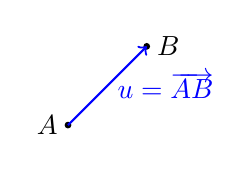
\begin{tikzpicture}
							\coordinate (a) at (0,0)  ;
							\coordinate (b) at (1,1) ;
							\filldraw[black] (a) circle (1pt);
							\filldraw[black] (b) circle (1pt);
							\draw[->, thick,blue] (a) node[left,black] {$A$} --  node[right, blue] {$u = \overrightarrow{AB}$}(b) node[right,black] {$B$};
						\end{tikzpicture}
					\end{center}
				}\pl{\rep{3cm}\pagebreak[4]}
\sld{\vfill\pagebreak[5]}%%%%%%%%%%%%%%%
			\item Relation de Chasles: $\forall A,B,C \in \Ee$ on a $\overrightarrow{AB} + \overrightarrow{BC} = \overrightarrow{AC}$.
				\sld{
\begin{center}
	\begin{tabular}{cc}
		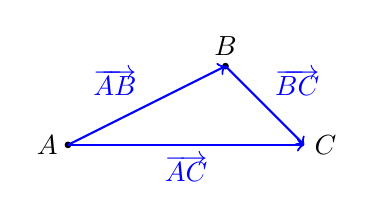
\begin{tikzpicture}
			\coordinate (a) at (0,0)  ;
			\coordinate (b) at (2,1) ;
			\coordinate (c) at (3,0) ;
			\filldraw[black] (a) circle (1pt);
			\filldraw[black] (b) circle (1pt);
			\draw[->, thick,blue] (a) node[left,black] {$A$} --  node[ above left, blue] {$\overrightarrow{AB}$}(b) node[above,black] {$B$};
			\draw[->, thick,blue] (b) --  node[above right, blue] {$\overrightarrow{BC}$}(c) node[right,black] {$C$};
			\draw[->, thick,blue] (a) --  node[below, blue] {$\overrightarrow{AC}$}(c);
		\end{tikzpicture} 
		&
		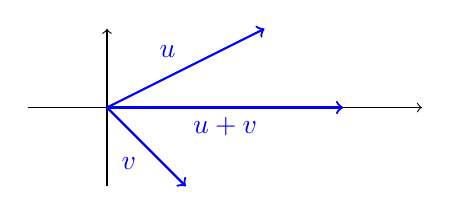
\begin{tikzpicture}
			\coordinate (a) at (0,0)  ;
			\coordinate (b) at (2,1) ;
			\coordinate (c) at (3,0) ;
			\draw[->] (0,-1) -- (0,1) ;
			\draw[->] (-1,0) -- (4,0) ;
			\draw[->, thick,blue] (a) --  node[ above left, blue] {$u$}(b);
			\draw[->, thick,blue] (a) --  node[below left, blue] {$v$}( 1,-1);
			\draw[->, thick,blue] (a) --  node[below, blue] {$u+v$}(c);
		\end{tikzpicture}
		\\
		dans $\Ee$ & dans $E$
	\end{tabular} 
\end{center}
} 

\pl{\rep{4cm}}
	\end{enumerate}
\end{enumerate}
En résumé, les éléments de $\Ee$ sont considérés comme des points (notés en majuscules) sur lesquels opèrent des vecteurs (notés en minuscules) de $E$. 

%La relation entre couples de points  et vecteurs est précisée dans la définition suivante~:%On peut axiomatiser la construction des espaces affines avec la définition suivante:
%\begin{definition}
%	Soit $E$ un \rev{}. Un espace affine dirigé par $E$ est un ensemble $\mathcal E$ non vide, muni d'une application $\varphi: \mathcal E \times \mathcal E \to E$ vérifiant les axiomes suivants:
%	\begin{enumerate}
%		\item pour tout $A,B,C\in \mathcal E$ on a $\varphi(A,C) = \varphi(A,B) +  \varphi(B,C)$ (\emph{relation de Chasles}),
%		\item pour tout $A \in \mathcal E$ et pour tout $x\in E$, il existe un unique $B \in \mathcal E$ tel que $x = \varphi(A,B)$ (\ie l'application $\varphi_A:M\mapsto\varphi(A,M)$ est une bijection de $\mathcal E$ dans $E$).
%	\end{enumerate}
%\end{definition}
%\begin{remark}
%	Dans le cas de l'espace, un couple de points $(A,B) \in \Ee^2$ est appelé un \emph{bipoint} auquel on associe le vecteur $\varphi(A,B) \in \R^3$ qui est noté $\overrightarrow{AB}$.
%\end{remark}

\sld{\vfill\pagebreak[5]}%%%%%%%%%%%%%%%
\subsection{Repère de l'espace} 

%\subsubsection{définitions}

\begin{definition}[(Repère cartésien)]
Un repère cartésien de l'espace $\Ee$ est la donnée d'un point $\Omega$ (l'origine du repère) et de trois vecteurs $(e_1,e_2,e_3)$ formant une base (\ie une famille libre g\'en\'eratrice) de l'espace $E$.
\end{definition}
\pl{\rep{3cm}}
\begin{definition}[(coordonnées cartésiennes)]
	Si $M$ est un point de $\Ee$ alors le vecteur $\overrightarrow{\Omega M}$ se décompose de façon unique sur les vecteurs de base:
	\[
		\overrightarrow{\Omega M} = x_1 e_1 + x_2 e_2 + x_3 e_3 
	\]
	Le triplet $\begin{psmallmatrix}x_1 \\ x_2 \\ x_3\end{psmallmatrix}_{\mathcal R}$ (ou plus simplement $\begin{psmallmatrix}x_1\\x_2\\ x_3\end{psmallmatrix}$ si il n'y a pas d'ambiguïtés) contient les coordonnées cartésiennes du point $M$ dans le repère $\mathcal R$.
\end{definition}
\pl{\rep{3cm}}

\sld{\vfill\pagebreak[5]}%%%%%%%%%%%%%%%
\begin{remark}
	Une fois une origine $\Omega$ de repère choisie, on peut identifier un point $M$ de $\Ee$ avec le vecteur $\overrightarrow{\Omega M} \in E$. 
	Alors, le choix d'un syst\`eme de coordonn\'ees permet de ramener tous les calculs \`a des calculs dans $\mathbb R^3.$
	Lorsque l'on ne précise pas la base, c'est que l'on se place dans l'espace vectoriel $E = \R^3$ muni de la base canonique composée des vecteurs $i = \begin{psmallmatrix}1\\0\\0\end{psmallmatrix}$, $j=\begin{psmallmatrix}0\\1\\0\end{psmallmatrix}$ et $k=\begin{psmallmatrix}0\\0\\1\end{psmallmatrix}$. 
\end{remark}

\sld{\vfill\pagebreak[5]}%%%%%%%%%%%%%%%


\bigskip

\begin{remark}{\bf\sffamily Changement de repère:} \label{rem_cdr} Soit deux repères cartésiens $\mathcal R =(\Omega,e_1,e_2,e_3) $ et $\mathcal R' =(\Omega',e_1',e_2',e_3') $ et un point $M$. On note:
\begin{itemize}
	\item $\begin{psmallmatrix}x\\ y \\z \end{psmallmatrix}_{\mathcal R}$ les coordonnées de $M$ dans $\mathcal R$ et $\begin{psmallmatrix}x'\\y'\\z' \end{psmallmatrix}_{\mathcal R'}$ les coordonnées de $M$ dans $\mathcal R'$
	\item $\begin{psmallmatrix}\alpha\\\beta\\\gamma \end{psmallmatrix}_{\mathcal R}$ les coordonnées de $\Omega'$ dans la $\mathcal R$.
	\item $\begin{psmallmatrix} a_{1,i}\\a_{2,i}\\a_{3,i} \end{psmallmatrix}_{\mathcal R}$ les coordonnées des $e_i'$ (pour $i=1,2,3$) dans $\mathcal R$.
\end{itemize}
%Pour passer d'un reprère à l'autre on a la formule suivante: 
Alors les coordonnées du point $M$ dans le repère $\mathcal R$ s'expriment en fonction des coordonnées de $M$ dans le repère $\mathcal R$:
\[
	\begin{cases}
		x = \alpha +a_{1,1}x'+ a_{1,2}y' +a_{1,3} z'\\
		y = \beta  +a_{2,1}x'+ a_{2,2}y' +a_{2,3} z'\\
		z = \gamma +a_{3,1}x'+ a_{3,2}y' +a_{3,3} z'
	\end{cases} \Leftrightarrow \begin{pmatrix}
		x\\y\\y
	\end{pmatrix}_{\mathcal R}=\begin{pmatrix}
		\alpha\\\beta\\\gamma
	\end{pmatrix}_{\mathcal R}+ \begin{pmatrix}
		a_{1,1} & a_{1,2} & a_{1,3}\\
		a_{2,1} & a_{2,2}& a_{2,3} \\
		a_{3,1} & a_{3,2} & a_{3,3}
	\end{pmatrix}_{\mathcal R \leftarrow \mathcal R'} \begin{pmatrix}
		x'\\y'\\z'
	\end{pmatrix}_{\mathcal R'}.
\]
\end{remark}

\sld{\vfill\pagebreak[5]}%%%%%%%%%%%%%%%


\begin{remark}
A propos des notations: un élément de $\R^n$ sera noté par convention $(x_1,\cdots, x_n)$ (c'est la donnée de $n$ réels). Lorsque l'on note $\begin{pmatrix}x_1 & \cdots & x_n\end{pmatrix}$  (resp. $\begin{psmallmatrix}x_1 \\ \vdots \\ x_n\end{psmallmatrix}$) on manipule en fait une matrice ligne (resp. colonne) dont les entrées sont les coordonnées d'un élément $(\tilde x_1, \cdots, \tilde x_n)$ dans une base donnée (ainsi lorsque les virgules disparaissent il y eut choix de base...). En général, les matrices colonnes représentent des vecteurs et les matrices lignes des formes linéaires (des fonctions linéaires à valeurs réelles).
\end{remark}
\sld{\vfill\pagebreak[5]}%%%%%%%%%%%%%%%
\subsection{Droites et plans affines}

\begin{definition}% [(Droite vectorielle, droite affine)]
Soit $\Ee$ un espace affine dirigé par un espace vectoriel $E$: 
	\begin{enumerate}
		\item Dans $E$: la \emph{droite vectorielle} engendrée par un vecteur $u\in E$ non-nul est l'ensemble des vecteurs colinéaires à $u$:
			\[
\redspace
				\vect(u) = \left\{ v\in E, \exists \lambda \in \R, v = \lambda u \right\} = \R u.
			\]
\pl{\rep{3cm}}
Si deux vecteurs $(u,v) \in E^2$ sont non-colinéaires, le \emph{plan vectoriel} engendré par $(u,v)$ est l'ensemble des vecteurs combinaisons linéaires de $u$ et $v$:
			\[
\redspace
				\vect(u,v) = \left\{ w\in E, \exists \lambda,\mu \in \R, w = \lambda u + \mu v \right\}.
			\]
\pl{\rep{3cm}}
		\item	Dans $\mathcal E$: la \emph{droite affine} $\mathcal D$ passant par un point $A$ et dirigée par un vecteur non-nul $u\in E$ est l'ensemble des points 
			\[
\redspace
			\mathcal D = \left\{D\in\Ee\  | \  D = A + \lambda u, \lambda \in \R \right\} \subset \Ee.
		\]
		On note $\mathcal D = A + \vect (u)$ et on dit que $\vect(u)$ est la direction de $\mathcal D$. De même, le \emph{plan affine} $\mathcal P$ dirigé par $u,v$ est 
		\[
\redspace
			\mathcal P =\left\{ A  + (\lambda u + \mu v), \lambda,\mu \in \R \right\} = A + \vect(u,v) \subset \Ee.
		\]
\pl{\rep{3cm}}
	\end{enumerate}
\end{definition}

\sld{\vfill\pagebreak[5]}%%%%%%%%%%%%%%%



%\pl{\pagebreak[5]}

\section{Calcul vectoriel}

\subsection{Produit scalaire}

\begin{definition}
	Soit $u =(u_1,u_2,u_3)$ et $v=(v_1,v_2,v_3)$ deux vecteurs de $\R^3$. Le produit scalaire de $u$ et $v$ est
	\[
		\prs{u,v} = u_1v_1 + u_2v_2 + u_3v_3.
	\]
et on définit la \emph{norme} d'un vecteur $u=(u_1,u_2,u_3)$ par
\[
	\norm{u}^2  = {u_1^2+u_2^2+u_3^2}.
\]
\end{definition}
\begin{remark}
    Le produit scalaire et la norme (au carrée) sont donc des relations polynômiales homogènes (de degré 2) des coordonnées de $u$ et $v$.
\end{remark}

\sld{\vfill\pagebreak[5]}%%%%%%%%%%%%%%%

\noindent{\bf\sffamily  Interprétation géométrique:} Soit $u$ et $v$ deux vecteurs  de $\R^3$ dont la norme est égale à 1:
\sld{
	\begin{center}
	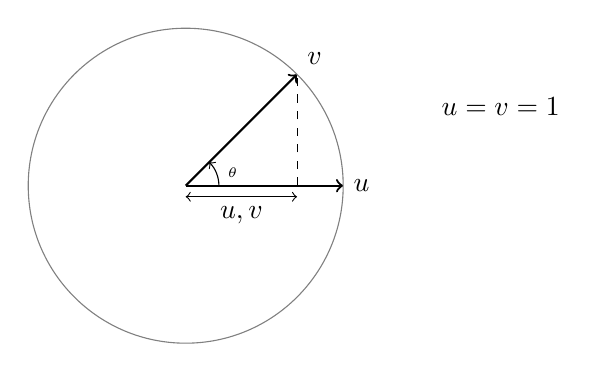
\begin{tikzpicture}[scale=2]
		\draw[->,thick] (0,0) -- (1,0) node [right] {$u$};
		\draw[->,thick] (0,0) -- (0.707106781,0.707106781) node [above right] {$v$};
		\draw[thin, gray] (0,0) circle (1);
		\draw[dashed] (0.707106781,0) -- (0.707106781,0.707106781);
		\draw[](0,0) -- (0.707106781,0); 
		\draw[<->,thin](0,-2pt) -- node[below]{$\prs{u,v}$}(0.707106781,-2pt); 
		\draw[->] (6pt,0) arc (0:45:6pt) node[midway, right=.5pt] {\tiny  $\theta$};
		\node at (2.0,.5) {$\snorm{u} = \snorm{v} =1$};
	\end{tikzpicture}
\end{center}
} \pl{\rep{4cm}}
Le produit scalaire de deux vecteurs unitaires est donc le cosinus de l'angle $\theta$ entre les vecteurs.
De plus, on a la formule suivante pour tout $u,v\in\R^3$:
\[
	\prs{u,v} = \norm{u}\norm{v} \cos(\theta).
\]
%et la propriété suivante (admise pour l'instant) 
%\[
	%\prs{u,v} \leq \norm{u}\norm{v}
%\]
En découle la majoration suivante \[\abs{\prs{u,v}} \leq \snorm{u}\snorm{v}\] avec cas d'égalité si $u$ et $v$ sont colinéaires.

%{\bf Interprétation en terme de projection ?}
%{\bf formule du cos de l'angle en fonction des coordonnée?}

\bigskip

\begin{proposition} Le produit scalaire satisfait aux règles de calculs suivantes:
	\begin{enumerate}
		\item \emph{Bilinéarité}: soient $u,v,w \in \R^3$ et $\lambda,\mu\in \R$:
			\begin{enumerate}
				\item  $\prs{\lambda u + \mu v, w} = \lambda \prs{u,w} + \mu \prs{v,w} $
				\item $\prs{u,\lambda v + \mu w} = \lambda \prs{u,v} + \mu \prs{u,w} $ 
			\end{enumerate}
		\item \emph{Symétrie}: soient $u,v\in\R^3$ $\prs{u,v} = \prs{v,u}$.
	\end{enumerate}
\end{proposition}

\begin{proof}
\pl{\rep{5cm}}	
\end{proof}

\sld{\vfill\pagebreak[5]}%%%%%%%%%%%%%%%

\begin{definition}
	\begin{enumerate}
		\item On dit que deux vecteurs sont \emph{orthogonaux} lorsque leur produit scalaire est nul.
		\item On dit qu'un vecteur est \emph{unitaire} lorsque sa norme vaut 1.
		\item On dit qu'une base est \emph{orthonormale} lorsque les trois vecteurs de la base sont orthogonaux deux à deux et unitaires. On utilise l'acronyme ``B.O.N.'' pour base orthonormale.
		\item On dit qu'un repère est \emph{orthonormé} lorsque sa base est orthonormale.
	\end{enumerate}
\end{definition}


%\subsubsection{Changement de base}

\begin{proposition}[(coordonnées d'un vecteur dans une B.O.N.)]
	Dans une base orthonormale $(e_1,e_2,e_3)$ de $\R^3$, un vecteur $u\in\R^3$ se décompose sous la forme\[
		u = \prs{e_1,u} e_1 + \prs{e_2,u} e_2 + \prs{e_3,u} e_3
	\]
\end{proposition}

\begin{proof}
\pl{\rep{4cm}}		
\end{proof}

\sld{\vfill\pagebreak[5]}%%%%%%%%%%%%%%%

\begin{proposition}[(Calcul du produit scalaire dans une B.O.N.)]
Si $(e_1,e_2,e_3)$ est une base orthonormale quelconque de $\R^3$ et si  $u = x_1 e_1 + x_2 e_2 + x_3 e_3$ et $v = y_1 e_1 + y_2 e_2 + y_3 e_3$ sont deux vecteurs de $\R^3$, alors le produit scalaire de $u$ et $v$ s'écrit:
\[
\prs{u,v} = x_1 y_1 + x_2y_2 + x_3y_3. 
\]
\end{proposition}

\begin{proof}
\pl{\rep{4cm}}		
\end{proof}

\sld{\vfill\pagebreak[5]}%%%%%%%%%%%%%%%

\begin{definition}
	On définit la \emph{distance} entre deux points $A$ et $B$ de l'espace $\Ee$ par:
	\[
		d(A,B) = \snorm{\overrightarrow{AB}}
	\]
	Si $\mathcal R$ est un repère orthonormé on a 
	\[
		d(A,B) = \sqrt{(x_1-y_1)^2+ (x_2-y_2)^2 + (x_3-y_3)^2 }
	\]
	où $\begin{psmallmatrix}
		x_1\\x_2\\x_3
	\end{psmallmatrix}_{}$ et $\begin{psmallmatrix}
		y_1\\y_2\\y_3
	\end{psmallmatrix}_{}$ sont les coordonnées dans $\mathcal R$ de $A$ et de $B$ respectivement.
\end{definition}

\sld{\vfill\pagebreak[5]}%%%%%%%%%%%%%%%
\section{Repérage}

\subsection{Orientation du plan et de l'espace}
Un repère orthonorm\'e $\mathcal R = \left(\Omega,e_1,e_2,e_3 \right)$ \'etant choisi, on rappelle que, pour exprimer les coordonn\'ees
d'un point dans un autre rep\`ere $\mathcal R' = \left(\Omega',e'_1,e'_2,e'_3 \right)$ il est n\'ecessaire d'utiliser la matrice de passage $B$
de la base $(e_1,e_2,e_3)$ \`a la base $(e'_1,e'_2,e'_3)$ (voir la {\bf Remarque \ref{rem_cdr}}). Si la nouvelle base est orthonom\'ee, on peut montrer que ${\rm det}(B) \in \{1,-1\}$ et a donc seulement deux valeurs possibles qui correspondent \`a deux orientations de l'espace. 

\begin{remark}
    D'un point de vue pratique, ceci s'illustre par le fait qu'un contorsionniste aussi dou\'e qu'il soit ne pourra pas superposer ses deux mains, droite et gauche.
\end{remark}

\sld{\vfill\pagebreak[5]}%%%%%%%%%%%%%%%

Il faut alors choisir une convention pour ``orienter l'espace'' et on se contente ici de décrire l'une des règles classiques  dite ``règle des 3 doigts de la main droite'' (il en existe d'autres comme la règle du ``bonhomme d'ampère'' ou la règle du ``tire bouchon'' qui suivent toutes la même convention): on dit qu'un repère est \emph{direct} si le pouce, l'index et le majeur de la main droite peuvent être placés (direction et sens) suivant les vecteurs $(e_1,e_2,e_3)$.
%On privilégiera bien sûr la représentation directe des axes $(Ox,Oy,Oz)$:

\begin{center}
	\begin{tabular}{c}
		\begin{tikzpicture}
			\def\side{2}
			%\draw[white,thick,->] (0,0,0) -- (0,0,\side+.3) node[below right,text width=1.4cm, align=center]{$z$ (majeur)} ;
			\draw[thick,->] (0,0,0) -- (\side+.3,0,0) node[right] {$x$};
			\draw[thick,->] (0,0,0) -- (0,\side+.3,0) node[above] {$y$};
			\draw[thick,->] (2,1) arc (0:90:1cm) node[above right,midway]{$+$};
		\end{tikzpicture}
	\\
		Repère direct du plan
	\end{tabular}
	\begin{tabular}{c}
		%\usetikzlibrary{3d}
\begin{tikzpicture}
	[%x={(-0.5cm,-0.5cm)},
%	    y={(1cm,0cm)},
%	    z={(0cm,1cm)}, 
		scale=1,
		fill opacity=1,%0.80,
		very thin,
	every node/.append style={transform shape}]

\def\ctr{1}
\def\side{2}
\def\sideT{.4}
\filldraw[color=blue!40] (-\sideT,-\sideT,0) -- (-\sideT,\side,0) -- (\side,\side,0) -- (\side,-\sideT,0) -- cycle;
\filldraw[color=gray!40] (-\sideT,0,-\sideT) -- (-\sideT,0,\side) -- (\side,0,\side) -- (\side,0,-\sideT) -- cycle;
\filldraw[color=green!40] (0,-\sideT,-\sideT) -- (0,-\sideT,\side) -- (0,\side,\side) -- (0,\side,-\sideT) -- cycle;

\def\sideT{0}
\filldraw[color=blue!40] (-\sideT,-\sideT,0) -- (-\sideT,\side,0) -- (\side,\side,0) -- (\side,-\sideT,0) -- cycle;
\filldraw[color=gray!40] (-\sideT,0,-\sideT) -- (-\sideT,0,\side) -- (\side,0,\side) -- (\side,0,-\sideT) -- cycle;
	\filldraw[color=green!40] (0,-\sideT,-\sideT) -- (0,-\sideT,\side) -- (0,\side,\side) -- (0,\side,-\sideT) -- cycle;

%	% face #3
	\begin{scope}[canvas is zx plane at y=0]
		\draw[thick,->] (1.5,1) arc (0:90:.5cm) node[above right,midway]{$+$};
		\node[rotate=90] at (\ctr/2,\ctr) {plan $xz$};
	\end{scope}
%	% face #2
	\begin{scope}[canvas is yx plane at z=0]
		\draw[thick,<-] (1.5,1) arc (0:90:.5cm) node[above right,midway]{$+$};
		\node[yscale=-1,rotate=-90] at (\ctr/2,\ctr) {plan $xy$};
	\end{scope} 
%
%      % face #1
	\begin{scope}[canvas is yz plane at x=0]
		\draw[thick,->] (1.5,1) arc (0:90:.5cm) node[above right,midway]{$+$};
		\node[rotate=-90] at (\ctr/2,\ctr) {plan $yz$};
	\end{scope}

	\draw[thick,->] (0,0,0) -- (\side+.3,0,0) node[right,text width=2cm, align=center] {$x$ (pouce)};
	\draw[thick,->] (0,0,0) -- (0,\side+.3,0) node[above,text width=2.1cm, align=center] {$y$ (index)};
	\draw[thick,->] (0,0,0) -- (0,0,\side+.3) node[below left,text width=2.4cm, align=center] {$z$ (majeur)};

\end{tikzpicture}
 
		% version with pst-figure3d
%\psset{viewpoint=50 20 30 rtp2xyz,Decran=50}
%\begin{pspicture}[solidmemory](-4,-4)(6,5)
%%\psset{unit=0.5}

%\psSolid[object=plan,action=draw,definition=equation,args={[0 0 1 0]}, base=-4 4 -4 4,fillcolor=black!15,fillstyle=solid,name=P0]
%\psProjection[object=texte,fontsize=100,linecolor=red,text=slice,phi=90,plan=P0]

%%\psSolid[object=cube,a=8,action=draw,name=A,linecolor=red]

%%\psSolid[object=plan,action=none,definition=solidface,args=A 4,name=P1]
%%\psProjection[object=texte,fontsize=50,text=lateral,phi=-90,plan=P1](-5,0)

%\psSolid[object=plan,action=draw,definition=equation,args={[0 1 0 0]},opacity=.2, base=-4 4 -4 4,fillcolor=black!15,name=P2]
%%\psProjection[object=texte,fontsize=50,text=axial,phi=90,plan=P2](0,7)
%%\psSolid[object=plan,action=none,definition=equation,args={[1 0 0 0]},name=P3]
%%\psProjection[object=texte,action=draw,fontsize=50,text=temporal,phi=90,plan=P3](4,8)
%\axesIIID(0,0,0)(4,4,4)
%\end{pspicture}

%\psset{unit=0.45}
%\psset{viewpoint=50 40 30 rtp2xyz,Decran=50}
%\psset{lightsrc=viewpoint}
%\begin{pspicture}(-7,-8)(7,8)
%\psSurface[ngrid=.25 .25](-4,-4)(4,4){((y^2)-(x^2))/4 }
%\end{pspicture}

%\psset{viewpoint=30 40 20 rtp2xyz,Decran=30}
  %\begin{pspicture}(-3.5,-3.5)(3.5,3.5)
%%  \axesIIID(2,2,2)(4,4,4)
   %\psSolid[object=cube,a=4,fillcolor=blue,opacity=0.2,action=draw*]%
   %\psSolid[object=sphere,r=1.5,linewidth=0.1pt,ngrid=20 20,fillcolor=red,opacity=0.2,action=draw*]%
   %\psSolid[object=vecteur,args=0 -2 0](2,2,-2)
   %\psSolid[object=vecteur,args=-2 0 0](2,2,-2)
   %\psSolid[object=vecteur,args=0 0 2](2,2,-2)
   %\psPoint(2,2,0.2){Z}\rput(Z){z}\psPoint(2,-0.2,-2){X}\rput(X){x}\psPoint(-0.2,2,-2){Y}\rput(Y){y}
   %\psPoint(2,-1.6,-2){a1}\psPoint(2,-1.6,2){a2}\pcline{<->}(a1)(a2)\ncput*{d}
   %\psPoint(2,-1.6,2){a1}\psPoint(-2,-1.6,2){a2}\pcline{<->}(a1)(a2)\ncput*{d}
   %\psPoint(-1.6,2,-2){a1}\psPoint(-1.6,2,2){a2}\pcline{<->}(a1)(a2)\ncput*{d}
   %\psPoint(0,0,0){a1}\psPoint(1,-1,0){a2}\pcline{->}(a1)(a2)\ncput*{r}
  %\end{pspicture}

%\begin{tikzpicture}
%\def\zlength{-0.5cm}
%\foreach \zangle [count=\i from 0] in {10,30,...,80}{
%\begin{scope}[shift={({mod(\i,2)*4cm},{-floor(\i/2)*4cm})}, 
    %x=(0:1cm), y=(90:1cm),z=(\zangle:\zlength)]
%%\def\zangle{80}
    %\def\sliceZ{0}
    %\def\side{2}
    %% draw plane
    %\filldraw[color=gray!40] (0,0,0) -- (0,0,\side) -- (\side,0,\side) -- (\side,0,0) -- cycle;
    %\filldraw[color=gray!40] (0,0,0) -- (0,\side,0) -- (\side,\side,0) -- (\side,0,0) -- cycle;
    %\filldraw[color=gray!40] (0,0,0) -- (0,0,\side) -- (,0\side,\side) -- (0,\side,0) -- cycle;
     %%\draw[dashed] (0,\sliceZ,0) -- (0,\sliceZ,\side) -- (\side,\sliceZ,\side) -- (\side,\sliceZ,0) -- cycle;
    %% draw axes
    %\draw[->] (0,0,0) -- (\side+.3,0,0) node[right] {$x$};
    %\draw[->] (0,0,0) -- (0,\side+.3,0) node[below] {$y$};
    %\draw[->] (0,0,0) -- (0,0,\side+.3) node[below] {$z$};
    %\node[cm={1,0,cos(\zangle),sin(\zangle),(0,0)}] at (1,1,0){plan $x-y$};
    %\node[cm={1,0,cos(\zangle),sin(\zangle),(0,0)}] at (1,0,1){plan $x-z$};
    %\node[cm={1,0,cos(\zangle),sin(\zangle),(0,0)}] at (0,1,1){plan $x-z$};
%\end{scope}
%}
%\end{tikzpicture}
\begin{tikzpicture}
    [%x={(-0.5cm,-0.5cm)},
%	    y={(1cm,0cm)},
%	    z={(0cm,1cm)}, 
    scale=1,
    fill opacity=1,%0.80,
    very thin,
    every node/.append style={transform shape}]
\newcommand\drawface{\draw[fill=gray!100] (-.2,-.2) rectangle (2,2)}

\def\ctr{1}
\def\side{2}
\def\sideT{.4}
\filldraw[color=green!40] (-\sideT,-\sideT,0) -- (-\sideT,\side,0) -- (\side,\side,0) -- (\side,-\sideT,0) -- cycle;
\filldraw[color=blue!40] (-\sideT,0,-\sideT) -- (-\sideT,0,\side) -- (\side,0,\side) -- (\side,0,-\sideT) -- cycle;
\filldraw[color=gray!40] (0,-\sideT,-\sideT) -- (0,-\sideT,\side) -- (0,\side,\side) -- (0,\side,-\sideT) -- cycle;

\def\sideT{0}
\filldraw[color=green!40] (-\sideT,-\sideT,0) -- (-\sideT,\side,0) -- (\side,\side,0) -- (\side,-\sideT,0) -- cycle;
\filldraw[color=blue!40] (-\sideT,0,-\sideT) -- (-\sideT,0,\side) -- (\side,0,\side) -- (\side,0,-\sideT) -- cycle;
\filldraw[color=gray!40] (0,-\sideT,-\sideT) -- (0,-\sideT,\side) -- (0,\side,\side) -- (0,\side,-\sideT) -- cycle;
	% face #3
	\begin{scope}[canvas is zx plane at y=0]
	   %\drawface;
		\draw[thick,->] (1.5,1) arc (0:90:.5cm) node[above right,midway]{$+$};
	   \node[rotate=90] at (\ctr/2,\ctr) {plan $xy$};
	\end{scope}
	% face #2
	\begin{scope}[canvas is yx plane at z=0]
	   %\drawface;
		\draw[thick,<-] (1.5,1) arc (0:90:.5cm) node[above right,midway]{$+$};
	   \node[yscale=-1,rotate=-90] at (\ctr/2,\ctr) {plan $yz$};
	\end{scope} 

       % face #1
	\begin{scope}[canvas is yz plane at x=0]
	    %\drawface;
		\draw[thick,->] (1.5,1) arc (0:90:.5cm) node[above right,midway]{$+$};
	    \node[rotate=-90] at (\ctr/2,\ctr) {plan $xz$};
	\end{scope}



	\draw[thick,->] (0,0,0) -- (\side+.3,0,0) node[right,text width=2.1cm, align=center] {$y$ (index)};
	\draw[thick,->] (0,0,0) -- (0,\side+.3,0) node[above,text width=2.4cm, align=center]{$z$ (majeur)} ;
	\draw[thick,->] (0,0,0) -- (0,0,\side+.3) node[below left,text width=2cm, align=center] {$x$ (pouce)};
\end{tikzpicture}

	\\
	Repères directs de l'espace
	\end{tabular}
\end{center}
Une permutation circulaire de trois vecteurs ne modifie pas son orientation et les deux repères ci-dessus sont directs. Si on change l'orientation d'un des vecteurs, on change l'orientation du repère (orientation \emph{indirecte}). Dans la suite de ce cours nous considèrerons toujours des repères directs.


\subsection{Coordonnées polaires}



Dans le plan muni d'un repère $(\Omega; e_1,e_2)$. Un point $M$ est décrit par une distance $r\in \R^+$ et un angle $\theta \in [0,2\pi[$. On a 
	\[\redspace
		\begin{cases}
			r^2 = x^2 + y^2\\
			\tan(\theta) = \frac{y}{x} 
		\end{cases} \Leftrightarrow \begin{cases}
			x = r\cos(\theta)\\
			y = r\sin(\theta)
		\end{cases}
	\]

	\begin{center}

	\pgfmathsetmacro{\sradius}{.2}
		\begin{tikzpicture}
			[scale=4,]

%draw the main coordinate system axes
		\draw[thick,->] (-.1,0) -- (.6,0) node[anchor=south]{$x$};
		\draw[thick,->] (0,-.1) -- (0,.6) node[anchor=north west]{$y$};


% (-z x y)

		\draw (.5, .5) node [circle,fill=red, inner sep=.02cm] () {};

		\draw[dashed,red] (.5, .5, 0) node[above right]{$M$}-- (.5,0,0);
		\draw[dashed,red] (.5, .5, 0) node[above]{}-- (0,.5,0);
		\draw[thick,red] (.5, .5, 0) -- node[midway,above left]{$r$} (0,0,0);

		\draw[thick,red] (0, 0, 0) -- (.5, .5,0);

		\draw[thick,->,red] (\sradius,0) arc (0:45:\sradius)node[midway,right]{$\theta$}  ;

		\end{tikzpicture}
	\end{center}
Attention, en l'état, il n'y a pas unicité des coordonnées polaires pour l'origine.
\sld{\vfill\pagebreak[5]}%%%%%%%%%%%%%%%
\subsection{Coordonnées cylindrique}


Dans l'espace avec $(\Omega;e_1,e_2,e_3)$ un repère orthonormé direct. On décrit la position d'un point $M$ par un triplet (distance, angle, hauteur)$=(r,\theta,z) \in \R^+ \times [0, 2\pi[ \times \R$. On a
\sld{\vfill\pagebreak[5]}%%%%%%%%%%%%%%%
\[
	\begin{cases}
		x = r\cos(\theta)\\
		y= r\sin(\theta) \\
		z=z
	\end{cases}
\Leftrightarrow
\begin{cases}
	r^2 = x^2 + y^2\\
	\tan(\theta) = \frac y x \\
	z=z
\end{cases}.
\]

\begin{center}
	\tdplotsetmaincoords{60}{110}

	\pgfmathsetmacro{\radius}{.707106781}
	\pgfmathsetmacro{\sradius}{.3}

%start tikz picture, and use the tdplot_main_coords style to implement the display 
%coordinate transformation provided by 3dplot
	\begin{tikzpicture}[scale=3,tdplot_main_coords,]

%draw the main coordinate system axes
		\draw[thick,->] (-.1,0,0) -- (.8,0,0) node[anchor=north east]{$x$};
		\draw[thick,->] (0,-.1,0) -- (0,.8,0) node[anchor=north west]{$y$};
		\draw[thick,->] (0,0,-.1) -- (0,0,.8) node[anchor=south]{$z$};


		%\draw[dashed] (\radius,0,\radius) arc (0:360:\radius);
		\draw[dashed] (\radius,0,0) arc (0:360:\radius);
% (-z x y)
%\draw (0, 1, 0) node [circle,fill=black, inner sep=.02cm] () {};
		\draw (0, 0, \radius) node [circle,fill=black, inner sep=.02cm] () {};
%\draw (1, 0, 0) node [circle,fill=black, inner sep=.02cm] () {};

		\draw (.5, .5, .6) node [circle,fill=red, inner sep=.02cm] () {};

                \draw[thick,red] (.5, .5, .6) node[above right]{$M$}--node[pos=.3, right]{$z$} (.5,.5,0);
		\draw[dashed,red] (.5, .5, .6) -- (0,0,0.6);
		\draw[dashed,red] (.5, .5, 0) node[above]{}-- (.5,0,0);
		\draw[dashed,red] (.5, .5, 0) node[above]{}-- (0,.5,0);
		\draw[thick,red] (.5, .5, 0) -- node[midway,right]{$r$} (0,0,0);
		\draw[dashed,red] (0, 0, 0) -- (.5, .5, .6);
		\draw[thick,->,red] (\sradius,0,0) arc (0:45:\sradius)node[midway,below]{$\theta$}  ;

		\fill[top color=blue!10!white,bottom color=blue!10!white,middle color=blue!10!white,shading=axis,opacity=0.1](\radius,0,0) arc (0:360:\radius);
%\fill[left color=gray!50!black,right color=gray!50!black,middle color=gray!50,shading=axis,opacity=0.25] (0,-\radius,0,0) arc (0:180:\radius) -- (.707106781,0,.707106781) arc (90:-90:\radius) -- (0-\radius,\radius) arc (180:360:\radius);
%\draw[->,blue] (0,-\radius,0) arc (-90:90:\radius) -- (0,.707106781,.707106781) arc (90:-90:\radius) -- (0,-\radius,0) -- cycle;

	%	\fill[top color=gray!90!,bottom color=gray!2,middle color=gray!30,shading=axis,opacity=0.1] (\radius,0,\radius) arc (0:360:\radius);

	\end{tikzpicture}
\end{center}


Attention, en l'état, il n'y a pas unicité des coordonnées cylindriques sur l'axe $Oz$.
\sld{\vfill\pagebreak[5]}%%%%%%%%%%%%%%%
\subsection{Coordonnées sphériques}

On se place toujours dans l'espace $(\Omega;e_1,e_2,e_3)$ muni d'un repère  orthonormé direct. De multiples conventions de coordonnées sphériques sont utilisées dans la littérature: on en décrit 2 ci-dessous. Mais attention, suivant les auteurs ou le contexte, une même quantité peut être notée de plusieurs manières. Bref, il faut se méfier et regarder attentivement les définitions. En cas de doute: faire un dessin.

\subsubsection{La convention (rayon,colatitude,longitude)}

Utilisée en mathématiques et en physique, on décrit un point $M$ de l'espace par le triplet: 
\begin{enumerate}
\item Rayon: c'est la distance à l'origine. Notation: $r \in \R^+$
\item Colatitude: angle entre l'axe vertical $(Oz)$ et le vecteur $\overrightarrow{OM}$. Notation: $\varphi \in [0,\pi]$
\item Longitude: c'est l'angle entre l'axe $(Ox)$ et le segment $\overrightarrow{OM'}$ où $M'$ est le projeté de $M$ sur le plan équatorial. Notation: $\theta \in [0,2\pi[$.
\end{enumerate}
\[
	\begin{cases}
		x = r\sin(\varphi) \cos(\theta)\\
		y = r \sin(\varphi) \sin(\theta)\\
	        z = r \cos(\varphi)
	\end{cases}
\Leftrightarrow
\begin{cases}
	r^2 = x^2+y^2+z^2 \\
	\cos(\varphi) = \frac{z}{\sqrt{x^2+y^2+z^2} } \\
	\tan(\theta) = \frac y x
\end{cases}
\]

\begin{center}
	\tdplotsetmaincoords{60}{110}

%define polar coordinates for some vector
%TODO: look into using 3d spherical coordinate system
	\pgfmathsetmacro{\radius}{1}
	\pgfmathsetmacro{\sradius}{.3}
	\pgfmathsetmacro{\thetavec}{0}
	\pgfmathsetmacro{\phivec}{0}

%start tikz picture, and use the tdplot_main_coords style to implement the display 
%coordinate transformation provided by 3dplot
        \begin{tikzpicture}[scale=2.5,tdplot_main_coords]
            \pgfmathsetmacro{\coordphi}{45}
            \pgfmathsetmacro{\coordtheta}{60}
            \pgfmathsetmacro{\coordr}{\radius}
            \pgfmathsetmacro\coordx{cos(\coordtheta)*sin(\coordphi) * \coordr}
            \pgfmathsetmacro\coordy{sin(\coordtheta)*sin(\coordphi) * \coordr}
            \pgfmathsetmacro\coordz{cos(\coordphi) * \coordr}

%draw the main coordinate system axes
            \draw[thick,->] (-.1,0,0) -- (1.1,0,0) node[anchor=north east]{$x$};
            \draw[thick,->] (0,-.1,0) -- (0,1.1,0) node[anchor=north west]{$y$};
            \draw[thick,->] (0,0,-.1) -- (0,0,1.1) node[anchor=south]{$z$};

            \tdplotsetthetaplanecoords{\phivec}

%draw some dashed arcs, demonstrating direct arc drawing
            \draw[dashed,tdplot_rotated_coords] (\radius,0,0) arc (0:90:\radius);
            \draw[dashed,tdplot_rotated_coords] (\radius,0,0) arc (0:-90:\radius);

            \draw[dashed] (\radius,0,0) arc (0:360:\radius);
            \shade[ball color=blue!10!white,opacity=0.2] (1cm,0) arc (0:-180:1cm and 5mm) arc (180:0:1cm and 1cm);
            % Draw intersection axes and unit sphere
            \draw (0, 1, 0) node [circle,fill=black, inner sep=.02cm] () {};
            \draw (0, 0, 1) node [circle,fill=black, inner sep=.02cm] () {};
            \draw (1, 0, 0) node [circle,fill=black, inner sep=.02cm] () {};

            % Draw point M and related lines
            \draw (\coordx, \coordy, \coordz) node [circle,fill=red, inner sep=.02cm] () {};

            \draw[dashed,red] (\coordx, \coordy, 0)  -- (\coordx,\coordy,\coordz) node[above]{$M$};
            \draw[dashed,red] (\coordx, \coordy, 0)  -- (\coordx,0,0);
            \draw[dashed,red] (\coordx, \coordy, 0)  -- (0,\coordy,0);
            \draw[dashed,red] (\coordx, \coordy, 0)  -- (0,0,0);

            \draw[thick,red] (0, 0, 0) -- node[midway,below right]{$r$} (\coordx, \coordy, \coordz);

            % Draw angle theta
            \draw[thick,->,red] (\sradius,0,0) arc (0:\coordtheta:\sradius)node[midway,below]{$\theta$}  ;

            % Draw angle phi
            \tdplotsetthetaplanecoords{\coordtheta}
            \draw[thick,<-,red,tdplot_rotated_coords] (\coordphi:\sradius) arc (\coordphi:0:\sradius) node[midway,above]{$\varphi$};
        \end{tikzpicture}

\end{center}



Attention, en l'état, il n'y a pas unicité des coordonnées sphériques sur l'axe $Oz$.

\subsubsection{La convention (rayon,latitude,longitude)}

Voici une autre convention (avec une référence plus ``géographique'), on décrit un point $M$ de l'espace par le triplet (rayon,latitude,longitude)$=(r,\delta,\theta) \in \R^+ \times \Big[-\frac{\pi}{2}, \frac{\pi}{2} \Big] \times [0,2\pi[$. On a 
\sld{\vfill\pagebreak[5]}%%%%%%%%%%%%%%%
\[
	\begin{cases}
		x = r\cos(\delta) \cos(\theta)\\
		y = r \cos(\delta) \sin(\theta) \\
	        z = r \sin(\delta)
	\end{cases}
\Leftrightarrow
\begin{cases}
	r^2 = x^2+y^2+z^2 \\
	\sin(\delta) = \frac{z}{\sqrt{x^2+y^2+z^2} } \\
	\tan(\theta) = \frac y x
\end{cases}
\]
On remarque que l'on a $\delta = \frac\pi2 - \varphi$ donnant $\cos(\delta) = \sin{\varphi}$ et $\sin(\delta) = \cos{\varphi}$.
\begin{center}
	\tdplotsetmaincoords{60}{110}

%define polar coordinates for some vector
%TODO: look into using 3d spherical coordinate system
	\pgfmathsetmacro{\radius}{1}
	\pgfmathsetmacro{\sradius}{.3}
	\pgfmathsetmacro{\thetavec}{0}
	\pgfmathsetmacro{\phivec}{0}

%start tikz picture, and use the tdplot_main_coords style to implement the display 
%coordinate transformation provided by 3dplot
        \begin{tikzpicture}[scale=2.5,tdplot_main_coords]
            \pgfmathsetmacro{\coordphi}{45}
            \pgfmathsetmacro{\coordtheta}{60}
            \pgfmathsetmacro{\coordr}{\radius}
            \pgfmathsetmacro\coordx{cos(\coordtheta)*sin(\coordphi) * \coordr}
            \pgfmathsetmacro\coordy{sin(\coordtheta)*sin(\coordphi) * \coordr}
            \pgfmathsetmacro\coordz{cos(\coordphi) * \coordr}

%draw the main coordinate system axes
            \draw[thick,->] (-.1,0,0) -- (1.1,0,0) node[anchor=north east]{$x$};
            \draw[thick,->] (0,-.1,0) -- (0,1.1,0) node[anchor=north west]{$y$};
            \draw[thick,->] (0,0,-.1) -- (0,0,1.1) node[anchor=south]{$z$};

            \tdplotsetthetaplanecoords{\phivec}

%draw some dashed arcs, demonstrating direct arc drawing
            \draw[dashed,tdplot_rotated_coords] (\radius,0,0) arc (0:90:\radius);
            \draw[dashed,tdplot_rotated_coords] (\radius,0,0) arc (0:-90:\radius);

            \draw[dashed] (\radius,0,0) arc (0:360:\radius);
            \shade[ball color=blue!10!white,opacity=0.2] (1cm,0) arc (0:-180:1cm and 5mm) arc (180:0:1cm and 1cm);
            % Draw intersection axes and unit sphere
            \draw (0, 1, 0) node [circle,fill=black, inner sep=.02cm] () {};
            \draw (0, 0, 1) node [circle,fill=black, inner sep=.02cm] () {};
            \draw (1, 0, 0) node [circle,fill=black, inner sep=.02cm] () {};

            % Draw point M and related lines
            \draw (\coordx, \coordy, \coordz) node [circle,fill=red, inner sep=.02cm] () {};

            \draw[dashed,red] (\coordx, \coordy, 0)  -- (\coordx,\coordy,\coordz) node[above]{$M$};
            \draw[dashed,red] (\coordx, \coordy, 0)  -- (\coordx,0,0);
            \draw[dashed,red] (\coordx, \coordy, 0)  -- (0,\coordy,0);
            \draw[dashed,red] (\coordx, \coordy, 0)  -- (0,0,0);

            \draw[thick,red] (0, 0, 0) -- node[midway,above left]{$r$} (\coordx, \coordy, \coordz);

            % Draw angle theta
            \draw[thick,->,red] (\sradius,0,0) arc (0:\coordtheta:\sradius)node[midway,below]{$\theta$}  ;

            % Draw angle phi
            \tdplotsetthetaplanecoords{\coordtheta}
            \draw[thick,<-,red,tdplot_rotated_coords] (\coordphi:\sradius) arc (\coordphi:90:\sradius) node[midway,right]{$\delta$};
        \end{tikzpicture}

\end{center}



Attention, en l'état, il n'y a pas unicité des coordonnées sphériques sur l'axe $Oz$.

%\addtocounter{chapter}{1}\chapter{Courbes paramétrées}

\sld{\includegraphics[width=\textwidth]{../figures/td4cinematique.png}}

\pl{Dans ce chapitre nous allons voir les propriétés fondamentales des courbes paramétrées.  Pour fixer les idées, commençons par présenter une courbe particulière: la \emph{cycloïde}. C'est la courbe que parcourt un point choisi de la roue d'un vélo, lorsque le vélo avance. Les coordonnées $(x,y)$ de ce point $M$ varient en fonction du temps:}
$$\left\{\begin{array}{rcl}
x(t) &=& r(t-\sin t) \\
y(t) &=& r(1-\cos t)
\end{array} \right.$$
où $r$ est le rayon de la roue.

\begin{center}
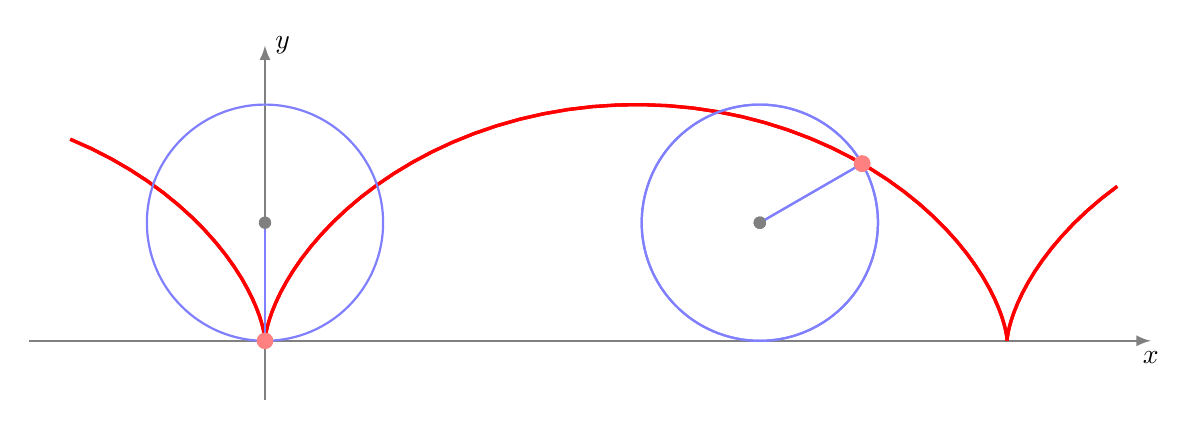
\begin{tikzpicture}[scale=1.5]

     \draw[->,>=latex,thick, gray] (-2,0)--(7.5,0) node[below,black] {$x$};
     \draw[->,>=latex,thick, gray] (0,-0.5)--(0,2.5) node[right,black] {$y$};

% Cycloide
\sld
\pl{
  \draw[red, very thick,domain=-0.75*pi:2.6*pi,samples=100] plot ({\x - sin(\x r)},{1 - cos(\x r)});
  }
\def\t{60}

\def\mkRoue#1#2{
\def\t{#1}
\begin{scope}[xshift=0.01745*\t cm, yshift=1 cm,rotate=-\t]
     \draw[thick, blue!#2]  (0,0) circle (1);
     \draw[thick, blue!#2] (0,0)--(0,-1);
     \fill[black!#2] (0,0) circle (1.5pt);
     \fill[red!#2] (0,-1) circle (2pt);
\end{scope}
}
\sld{%\uncover<1->}{
\mkRoue{0}{50};
%\mkRoue{80}{50};
\mkRoue{240}{50};
}

\pl{
\mkRoue{240}{50};
}
%\beameronly {\uncover<3->}{\mkRoue{160}{100};}

\end{tikzpicture}
\end{center}

La cycloïde a des propriétés remarquables. Par exemple, la cycloïde renversée est une courbe \emph{brachistochrone}: c'est-à-dire que c'est la courbe qui permet à une bille (soumis à la seule gravité) d'arriver le plus vite possible d'un point $A$ à un point $B$.  Contrairement à ce que l'on pourrait croire ce n'est pas une ligne droite, mais bel et bien un arc de cycloïde.  Sur le dessin suivant les deux billes sont lâchées en $A$ à l'instant $t_0$, l'une sur le segment $[AB]$ ; elle aura donc une accélération constante.  La seconde parcourt la cycloïde renversée, ayant une tangente verticale en $A$ et passant par $B$.  La bille accélère beaucoup au début et elle atteint $B$ bien avant l'autre bille (à l'instant $t_4$ sur le dessin).  Notez que la bille passe même par des positions en-dessous de $B$ (par exemple en $t_3$).  

\begin{center}

    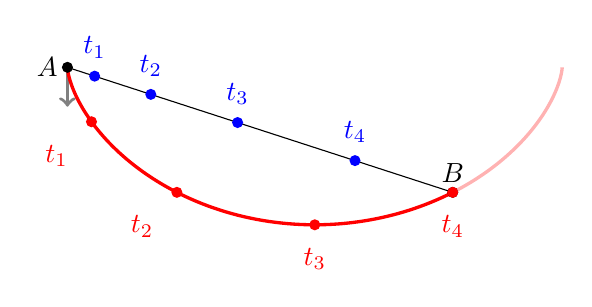
\begin{tikzpicture}
%
%      \draw[->,>=latex,thick, gray] (-2,0)--(3.5,0) node[below,black] {$x$};
%      \draw[->,>=latex,thick, gray] (0,-2.5)--(0,2.5) node[right,black] {$y$};

    %tangente à l'origine
        \draw[gray,very thick,->] (0,0) -- (0,-.5);
% Cycloide

        \def\T{1.3*pi};  % Do not change
        \def\a{\T-sin(deg(\T))};
        \def\b{-1+cos(deg(\T))};
        \draw (0,0)--({\a},{\b});


        \draw[red, very thick,domain=0:\T,samples=100] plot ({\x - sin(\x r)},{-1+ cos(\x r)});
        \draw[red!30, very thick,domain= \T:2*pi,samples=100] plot ({\x - sin(\x r)},{-1+ cos(\x r)});

% \def\x{4.08};
% \fill[black] ({\x - sin(\x r)},{-1+ cos(\x r)})circle (2pt) ;

        \fill[black] (0,0) circle (2pt) node[left] {$A$};
        \fill[black] ({\a},{\b}) circle (2pt) node[above] {$B$};


% Variables: time=angle, transparency, index, position index
        \def\mkPlot#1#2#3#4{
            \def\t{#1}

   % Cycloide
            \def\newa{\t-sin(deg(\t))};
            \def\newb{-1+cos(deg(\t))};
            \fill[red!#2] ({\newa},{\newb}) circle (2pt) node[#4=5pt] {$t_{#3}$};

  % Line
            \def\r{sqrt((\a)*(\a)+(\b)*(\b))};
            \def\mycoeff{0.29}
    \fill[blue]({-0.5*(\mycoeff)*(\b)/(\r))*(\a)*\t*\t},{-0.5*(\mycoeff)*(\b)/(\r))*(\b)*\t*\t}) circle (2pt) node[above=3pt] {$t_{#3}$};

% Attention le coeff \mycoeff 0.25 ci-dessus est au pif
% Voir http://www.mathcurve.com
}

\mkPlot{0.4*pi}{100}{1}{below left};
\mkPlot{0.7*pi}{100}{2}{below left};
\mkPlot{1.0*pi}{100}{3}{below};
\mkPlot{1.3*pi}{100}{4}{below};

\end{tikzpicture}
\end{center}





Dans ce chapitre, $E$ désigne l'espace vectoriel $\R^n$ muni de sa base canonique. La norme $\ncd$ désigne la norme euclidienne: pour $x\in E$ ayant pour coordonnées $\begin{pmatrix}x_1\\\vdots\\x_n\end{pmatrix}$, on a 
\[
    \snorm{x} = \sqrt{x_1^2 + \cdots + x_n^2}.
\]
Tous les résultats de ce chapitre s'étendent aux $\R$ espaces vectoriels de dimension finie munis d'une base quelconque.

\section[Fonctions vectorielles]{Fonctions vectorielles d'une variable réelle}

\subsection{Définition et structure d'espace vectoriel}

\begin{definition}
	%Soit $(E,\snorm{\cdot})$ un \rev. 
	Soit $E=\R^n$.  
	Une fonction vectorielle d'une variable réelle est une application définie sur un sous ensemble $I\subset \R$ et à valeurs dans $E$. On note $t\mapsto f(t)$. L'ensemble des applications $I\to E$ se notera $\mathcal F (I,E)$ ou parfois $E^I$.
\end{definition}

%Supposons que $E$ soit un \rev de dimension finie $n$.
Soit $\mathcal B=(e_1,\cdots,e_n)$ la base canonique de $E=\R^n$. Alors toute $f\in\mathcal F(I,E)$  est définie par ses \emph{fonctions coordonnées} $f_i: I \to \R$:
\[\redspace
t\mapsto f(t) = f_1(t) e_1 + f_2(t) e_2 + \cdots + f_n(t) e_n.
\]
En pratique, on considère pratiquement toujours le cas $E=\R^2$ ou $\R^3$ munis de leur base canonique respective. On note alors:
\[\redspace
	t\mapsto \begin{pmatrix}f_1(t)\\f_2(t)\end{pmatrix}  \qquad \text{ ou } 	\qquad t\mapsto \begin{pmatrix}f_1(t)\\f_2(t)\\f_3(t)\end{pmatrix}  
\]
En résumé, considérer une fonction vectorielle d'une variable réelle, c'est simplement ``regrouper'' $n$ fonctions réelles de la variable réelle.

\sld{\vfill\pagebreak[5]}%%%%%%%%%%%%%%%


\begin{exemple}
	Si $E=\R^2$ et $I=[0,2]$ le graphe de %la fonction vectorielle 
	$t\mapsto (t\cos(6t),t\sin(6t))$ est un sous ensemble de $\R\times\R^2\simeq\R^3$:
	\begin{center}
	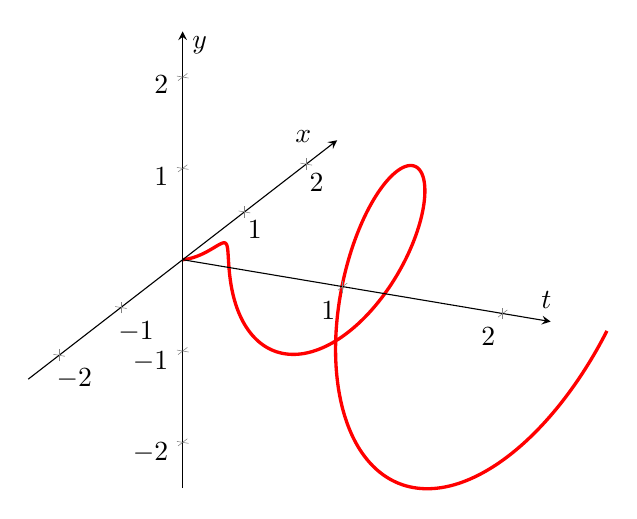
\begin{tikzpicture}[scale=1]\pgfplotsset{compat=1.8}
			\begin{axis}[enlargelimits=true,axis lines=center, axis on top, xlabel={$t$}, ylabel={$x$}, zlabel={$y$}, %axis equal,view={35}{340},,
				ymin=-2.5,ymax=2.5,zmin=-2.5,zmax=2.5,xmin=-0,xmax=2.3,	y post scale=1.8,z post scale=1.8]
				\addplot3[samples=500, very thick,red, domain = 0:2, samples y =0] ({x},{x*cos(6*deg(x))},{ x*sin(6*deg(x))});
			\end{axis}
		\end{tikzpicture}
	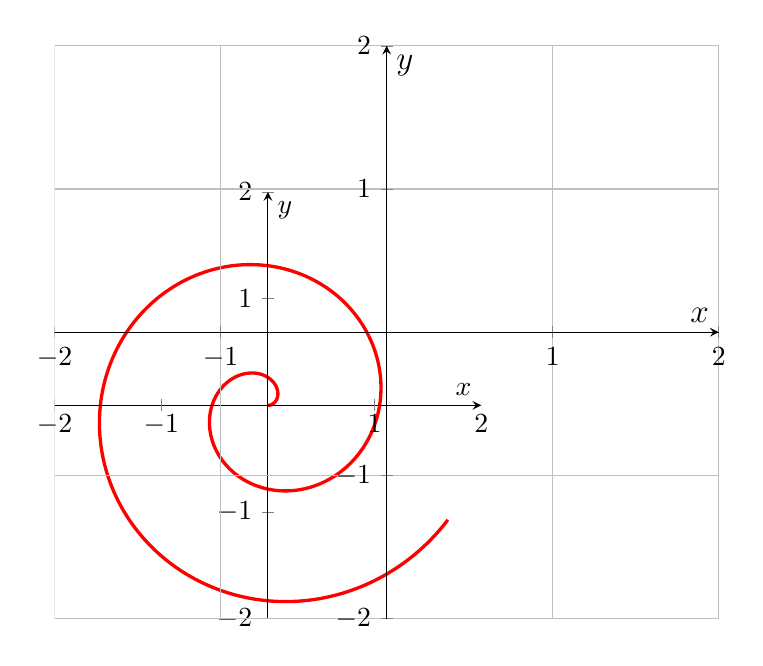
\begin{tikzpicture}\pgfplotsset{compat=1.8}
				\sld{\begin{axis}[height=7cm,width=7cm,enlargelimits=true,grid=major,  axis lines=center, axis on top, xlabel={$x$}, ylabel={$x$}, zlabel={$y$}, axis equal,view={90}{0},,
				ymin=-2,ymax=2,zmin=-2,zmax=2,xmin=0,xmax=2]
				\addplot3[grid=both,samples=500, very thick,red, domain = 0:2, samples y =0] ({x},{x*cos(6*deg(x))},{ x*sin(6*deg(x))});
			\end{axis}}
				\pl{\begin{axis}[ scale only axis, grid=major, axis lines=middle, inner axis line style={=>}, xlabel={\large $x$}, ylabel={\large $y$}, ytick={-2,-1,...,2}, xtick={-2,-1,...,2}, ymin=-2, ymax=2, xmin=-2, xmax=2, samples=50 ]
\addplot[color=black,thin] {0};

			\end{axis}}
		\end{tikzpicture}
	\end{center}
\end{exemple}


\bigskip

\sld{\vfill\pagebreak[5]}%%%%%%%%%%%%%%%

On peut munir $\mathcal F(I,E)$ de l'addition $\mathcal F(I,E) \times \mathcal F(I,E) \to \mathcal F(I,E)$ définie par  $(f,g) \mapsto f+g$  avec
\[
	(f+g)(t) = f(t)+g(t), \qquad \text{ pour tout $t\in I$.}
\]
Cette opération est associative, commutative, admet un élément neutre (la fonction nulle $t\mapsto 0$) et chaque $f\in \mathcal F(I,E)$ admet un opposé $-f$ définit par $(-f)(t)= -f(t)$. De plus pour tout $\alpha\in\R$ l'application $(\alpha,f) \mapsto \alpha f$ est une application $\R\times \mathcal F(I,E) \to \mathcal F(I,E)$ (appelée multiplication externe). On a 
\[
	(\alpha f) (t) = \alpha f(t), \qquad \text{ pour tout $t\in I$.}
\]
On a le résultat suivant:
\begin{proposition}\label{prop.revFIE}
	L'espace $\mathcal F(I,E)$ est un \rev{} (de dimension infinie). 
\end{proposition}

\begin{proof}
    La démonstration ne pose pas de problème particulier: il faut vérifier un à un les axiomes des \rev. Noter que c'est le fait que l'espace d'arrivée $E$ soit un \rev{} qui fait fonctionner le tout.
\end{proof}


\subsection{Limite et continuité}

%On note $(E,\snorm{\cdot})$ un \rev de dimension finie et $ $ une base de $E$.
On note toujours $E=\R^n$ muni de la base canonique et de la norme euclidienne. Soit $I$ un intervalle ouvert de $\R$ et $f:I\to E$ alors on note $f_i: I \to \R$ les fonctions coordonnées pour $i=1,\cdots,n$. Avec ces notations on a:
\begin{definition}[(limite)]
	On dit que $f$ admet une limite $\ell = \begin{psmallmatrix}\ell_1\\\vdots\\\ell_n\end{psmallmatrix}\in E$ quand $t$ tend vers $a\in I$ si $\lim_{t\to a}\limits  f_i(t) = \ell_i$ pour tout $i=1,\cdots,n$. Dans ce cas on a
	\[
		\lim_{t\to a} f(t) = \begin{pmatrix}\lim_{t\to a}\limits f_1(t) \\ \vdots \\ \lim_{t\to a}\limits f_n(t)\end{pmatrix} = \begin{pmatrix}\ell_1\\ \vdots \\ \ell_n\end{pmatrix} = \ell
	\]
\end{definition}
En bref, $f$ admet une limite en $a$ si toutes ses fonctions coordonnées convergent en $a$. Cette définition équivaut à $\lim_{t\to a} \limits \| f(t) - \ell\| =0 $ et on peut se ramener à la limite d'une fonction réelle. Si la limite existe, elle est unique.

\pl{\rep{4cm}}


\begin{remark}
	Cette définition s'adapte sans difficultés aux notions de limites à droite (\ie quand $t\to a$ avec $t>a$) noté $\lim_{t\to a^+} \limits f(t) $ ou $f(a^+)$ et limite à gauche  (\ie quand $t\to a$ avec $t<a$) notée $\lim_{t\to a^-}\limits  f (t)$ ou $f(a^-)$. Ainsi, si $f(a^+) = f(a^-) = \ell$ alors $f$ admet $\ell$ pour limite en $a$. 
\end{remark}

De même que dans le cas des fonctions réelles on a la caractérisation suivante:

\begin{proposition}[(caractérisation séquentielle)]
    Pour que $f$ admette une limite $\ell \in E$ en $a\in I$ il faut et il suffit que pour toute suite $(u_n)_{n\in\N}$ de $I$ telle que $\lim_n u_n = a \in I$ on ait $\lim_n f(u_n)= \ell \in E$ (ou autrement dit que pour tout $i=1,\cdots,n$ on a $f_i(u_n) \to \ell_i$ quand $n\to+\infty$). 
\end{proposition}

\sld{\vfill\pagebreak[5]}%%%%%%%%%%%%%%%
On rappelle que la continuité est une notion \emph{locale}. Plus précisément on a:
\begin{definition} 
	Soit $f:I\to E$ une fonction vectorielle. On dit que $f$ est \emph{continue} en $a\in I$ si 
\[ \redspace
	\lim_{t\to a }f(t)= f(a)
\]
En d'autre termes, $f$ est continue en $a\in I$  si
\[ \redspace
	\lim_{t\to a} \snorm{f(t) - f(a)} = 0
\]
\end{definition}
	Ainsi, une fonction vectorielle est dite continue en $a$ si toutes ses fonctions coordonnées sont continues en $a$. Si l'intervalle $I$ est minoré (resp. majoré), on peut étendre facilement la définition de continuité à droite (resp. à gauche) pour le réel $a$ situé à l'extrémité inférieure (resp. supérieure) de $I$.	
	
Une fonction est continue sur un intervalle $I$ si et seulement si elle est continue en tout point de $I$. Dans la suite, on notera $\mathcal C^0(I,E)$ l'ensemble des fonctions continues de $I\subset \R$ dans $E$.
	\begin{proposition}
		L'espace fonctionnel $\mathcal C^0(I,E)$ est un \rev.
	\end{proposition}

	\begin{proof}
	Même remarque que pour la preuve de la Proposition \ref{prop.revFIE}	
	\end{proof}

\sld{\vfill\pagebreak[5]}%%%%%%%%%%%%%%%
	\begin{definition}
		On dit que $f:I\to E$ est \emph{uniformément continue} sur $I$ si, pour tout $\varepsilon>0$, il existe $\delta>0$ tel que, pour tout $t,t'\in I$ on a 
		\[
			\abs{t-t'} <\delta \Rightarrow \snorm{f(t) - f(t')} < \varepsilon.
		\]
	\end{definition}

	\begin{proposition}[(Théorème de Heine)]
		Soit $I$ un intervalle fermé et borné de $\R$ et $E=\R^n$. Toute application continue de $I$ dans $E$ est uniformément continue sur $I$.
	\end{proposition}

\sld{\vfill\pagebreak[5]}%%%%%%%%%%%%%%%
\subsection{Dérivabilité}

Soit $E=\R^n$ muni de la base canonique et de la norme euclidienne. Soit $I$ un intervalle ouvert de $\R$ et $f:I\to E$ alors on note $f_i: I \to \R$ les fonctions coordonnées pour $i=1,\cdots,n$. Avec ces notations on a:
\begin{definition}[(dérivabilité)] 
	Soit $f:I\to E$ une fonction vectorielle. On dit que $f$ est dérivable en $a\in I$ si toutes les fonctions coordonnées de $f$ sont dérivables en $a$. On note
\[
	f'(a)= \begin{pmatrix}f_1'(a) \\ \vdots \\ f_n'(a)\end{pmatrix}
\]
\end{definition}
La dérivabilité est comme la continuité une définition locale. Une fonction vectorielle $f$ est dite dérivable sur $I$ si elle est dérivable en tout point de $I$.
%On dit que $f$ est différentiable en $a \in I$ s'il existe une fonction $h \mapsto \varepsilon(h)$ de $I$ dans $E$ et un vecteur $\ell \in E$ vérifiant,
%\[
%	f(a+h) -f(a) = h \ell + h\varphi(h)
%\]

\sld{\vfill\pagebreak[5]}%%%%%%%%%%%%%%%

Bien sûr, si les fonctions coordonnées sont suffisamment régulières, on peut généraliser la définition aux dérivées d'ordres supérieurs. On alors $f'' = \begin{psmallmatrix}
	f''_1\\ \vdots\\ f''_n
\end{psmallmatrix}$ et plus généralement on note $f^{(k)}= \begin{psmallmatrix}
	f^{(k)}_1\\ \vdots\\ f^{(k)}_n
\end{psmallmatrix}$ le vecteurs des dérivées $k$-ème. On notera enfin $\mathcal C^k(I, E)$ l'ensemble des fonctions vectorielles admettant une dérivée d'ordre $k$ continue (\ie dont les fonctions coordonnées sont $\mathcal C^k(I,\R)$).


\sld{\vfill\pagebreak[5]}%%%%%%%%%%%%%%%

On rappelle que le théorème des accroissements finis (TAF) pour une fonction $f:[a,b] \to \R$. Si $f$ est continue sur $[a,b]$ et dérivable sur $]a,b[$ alors il existe $c \in]a,b[$ tel que 
	\[f(b) - f(a) =  f'(c) (b-a) \]
Sous cette forme, le théorème ne se généralise pas aux fonctions vectorielles.
\begin{exemple}
 On considère la fonction vectorielle $t\mapsto (\sin(t) , \sin(2t))$.	
 \pl{\rep{4cm}}
\end{exemple}

\sld{\vfill\pagebreak[5]}%%%%%%%%%%%%%%%

On a le résultat plus faible suivant mais qui est valable pour les fonctions vectorielles et numériques:
\begin{theorem}[(Inégalité des accroissements finis)]
	Soit $f:[a,b] \to E$ une fonction vectorielle continue sur $[a,b]$ et dérivable sur $]a,b[$. %On suppose qu'il existe $\varphi:[a,b] \to \R$ continue sur $[a,b]$, dérivable sur $]a,b[$ et telle qu'en tout point $x$ de $]a,b[$ on ait l'inégalité
		%\[
	%		\snorm{f'(x)} \leq \varphi'(x)
	%	\]
	%	Alors, on a aussi la majoration suivante:
	%	\[
	%		\snorm{f(a) - f(b)} \leq \varphi(b) - \varphi(a)
	%	\]
	On suppose qu'il existe $M\geq 0$ tel que 
	\[
		\snorm{f'(x)} \leq M.
	\]
pour tout $x\in ]a,b[$. ALors 
	\[
		\snorm{f(a) -f(b) } \leq M (b-a).
	\]
		\label{TAF}
\end{theorem}


\sld{\vfill\pagebreak[5]}%%%%%%%%%%%%%%%

\section{Courbes paramétrées}

\subsection{Définitions}

Soit $E$ un \rev{}.

\begin{definition}
	On appelle \emph{courbe paramétrée} (on dit aussi \emph{arc paramétrée}) de $E$, un couple $\Gamma = (I,\phi)$ formé d'un intervalle de $I$ de $\R$ et d'une application $\phi:I \to E$ de classe $\Cc^1$ sur $I$. L'image $\phi(I) \subset E$ de $\phi$ est le \emph{support} de la courbe paramétrée $\Gamma$. 
\end{definition}

\pl{\rep{3cm}}

Lorsque $\phi$ est de classe $\Cc^k$ on dit que la courbe paramétrée est de classe $\Cc^k$.

\begin{exemple}
	\sld{	
\begin{enumerate}
\item Soit $E =\R^3$, un point $A\in E$ et $v\in E$ alors $\phi: t \mapsto A + tv$ pour tout $t\in\R$ est une droite affine passant par $A$ et de direction $v$.

\item Soit $I=[0,2\pi]$, $E=\R^2$ et $a,b>0$. Alors $\phi: t \mapsto (a\cos(t),b\sin(t))$ est une ellipse.
\end{enumerate}
}

\pl{\rep{3cm}}
\end{exemple}

\sld{\vfill\pagebreak[5]}%%%%%%%%%%%%%%%

\begin{exemple}
	$E =\R^3$ et $\phi: t \mapsto \left( \cos t, \sin t , \sinh t \right) \frac{1}{\cosh t} $ pour tout $t\in\R$.
	\begin{center}
		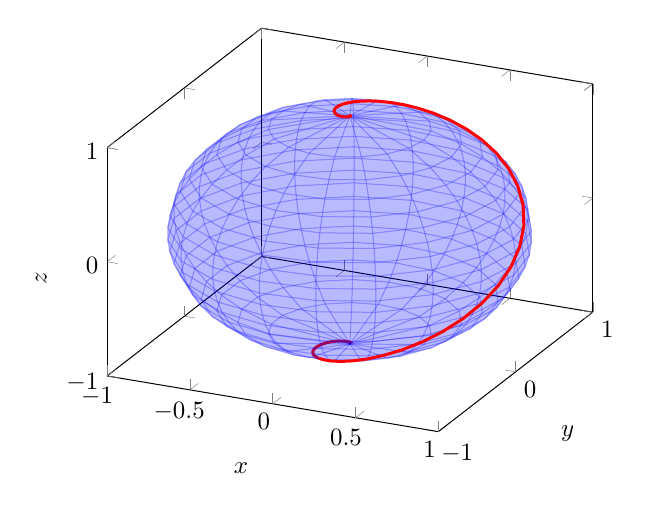
\begin{tikzpicture}[scale=.9]
			\begin{axis}[xlabel = $x$,ylabel=$y$,zlabel=$z$,, xmin=-1,xmax=1,ymin=-1,ymax=1,zmin=-1,zmax=1]
				\addplot3[, axis equal,samples=100,red, very thick, domain = -5:-pi/2, samples y =0] ({cos(deg(x))/cosh(x)},{sin(deg(x))/cosh(x)},{tanh(x)});
				\addplot3[surf,shader=flat,opacity=.15,z buffer=sort,blue,samples=20,domain=-1:1,y domain=0:2*pi]
({sqrt(1-x^2) * cos(deg(y))},
{sqrt( 1-x^2 ) * sin(deg(y))},
x);
				\addplot3[ axis equal,samples=100,red, very thick, domain = -pi/2:10, samples y =0] ({cos(deg(x))/cosh(x)},{sin(deg(x))/cosh(x)},{tanh(x)});
			\end{axis}
		\end{tikzpicture}
	\end{center}
	Pour des détails concernant la fonction $t\mapsto \cosh t$ on pourra voir \url{http://exo7.emath.fr/cours/ch_chainette.pdf}. Concernant les fonctions de la trigonométrie hyperbolique voir \cite{tt1} ou \cite{exo7} Chapitre 10.
\pl{\rep{10cm}}
\end{exemple}

\sld{\vfill\pagebreak[5]}%%%%%%%%%%%%%%%

\begin{exemple} Le trèfle gauche: $t\mapsto\begin{pmatrix}
			\cos(t) + 2\cos(2t) \\
			\sin(t) - 2\sin(2t)\\
			-2\sin(3t)
		\end{pmatrix}$
	
	\begin{center}
		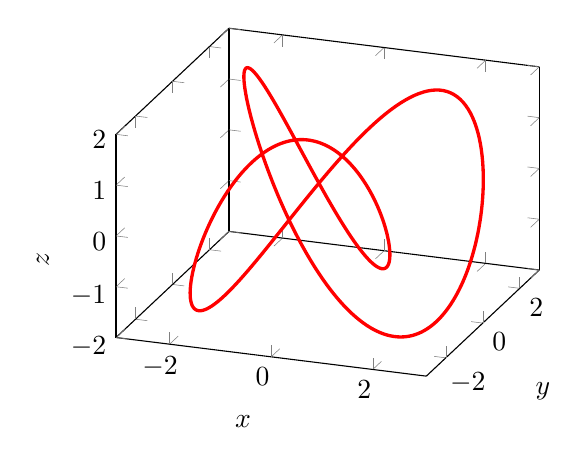
\begin{tikzpicture}
			\begin{axis}[height=6cm,xlabel = $x$,ylabel=$y$,zlabel=$z$,view={20}{20},  axis equal,xmin=-3,xmax=3,ymin=-3,ymax=3,zmin=-2,zmax=2]
				\addplot3[samples=500, very thick,red, domain = -0:10, samples y =0] ({cos(deg(x)) + 2*cos(deg(2*x))},{sin(deg(x)) - 2* sin(deg(2*x))},{-2*sin(deg(3*x))});
			\end{axis}
\end{tikzpicture}
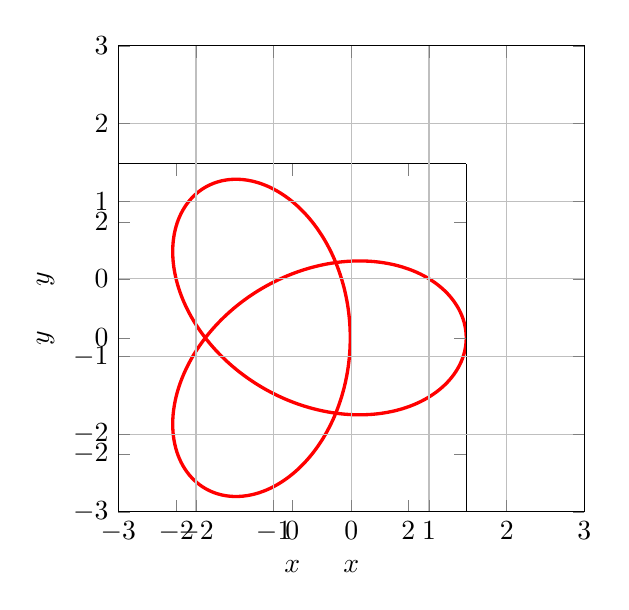
\begin{tikzpicture}%
	\sld{\begin{axis}[height=6cm,width=6cm, xlabel = $x$,ylabel=$y$,view={0}{90}, xmin=-3,xmax=3,ymin=-3,ymax=3,zmin=-3,zmax=3]
			\addplot3[samples=500, very thick,red, domain = -0:10, samples y =0] ({cos(deg(x)) + 2*cos(deg(2*x))},{sin(deg(x)) - 2* sin(deg(2*x))},{-2*sin(deg(3*x))});
			\end{axis}}%
	\pl{\begin{axis}[height=7.5cm,width=7.5cm, grid=major, inner axis line style={=>}, xlabel={$x$}, ylabel={$y$}, ytick={-3,-2,...,3}, xtick={-3,-2,...,3}, ymin=-3, ymax=3, xmin=-3, xmax=3, samples=5 ]\addplot[color=gray,thin] {10};
			\end{axis}}
\end{tikzpicture}
	\end{center}
\end{exemple}
\begin{definition}
    Une courbe paramétrée continue $\Gamma =(I,\phi)$ est \emph{simple} si tout point $M = \phi \in \phi(I)$ a un unique antécédents par  $\phi$.
            \begin{center}
                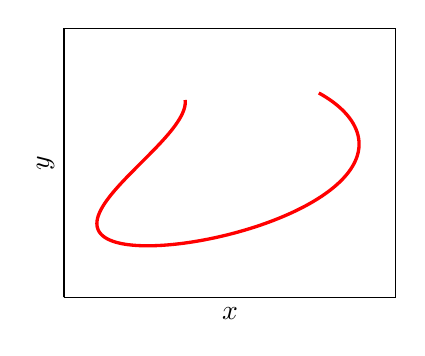
\begin{tikzpicture}
                    \begin{axis}[height=3cm,xlabel = $x$,ylabel=$y$,zlabel=$z$,height=5cm, axis equal,view={0}{90},, xmin=-2.5,xmax=1.5,ymin=-1,ymax=1,zmin=-0,zmax=0,xtick=\empty, ytick=\empty,]
                        \addplot3[samples=500, very thick,red, domain = -2:.5, samples y =0] ({cos(deg(3*x)) + x},{ sin(deg(2*x))},{0});
                    \end{axis}
                \end{tikzpicture}
            \end{center}\sld{\vfill\pagebreak[5]}%%%%%%%%%%%%%%%
            Un point \emph{multiple} est un point qui possède plusieurs antécédent par $\phi$.
    \begin{enumerate}
    %\item \emph{ $\boldsymbol{\Cc^1}$ par morceau} si $I=[a,b]$ et il existe une subdivision $a_0=a < a_1 < \cdots< b=a_m$ telle que la restriction $\Gamma_{a_i,a_{i+1}} = ([a_{i-1},a_{i}],\phi)$ est de classe $\Cc^1$ pour tout $i=\left\{ 0,\cdots,m-1 \right\}$.
        %\begin{center}
            %\begin{tikzpicture}
                %\begin{axis}[height=3cm,xlabel = $x$,ylabel=$y$,zlabel=$z$, height=5cm,axis equal,view={0}{90},, xmin=-2,xmax=3,ymin=-3,ymax=3,zmin=-0,zmax=0,xtick=\empty, ytick=\empty,]
                %\addplot3[samples=500, very thick,red, domain = -0:pi*3/2, samples y =0] ({cos(deg(2*x)) + 2*cos(deg(x))},{2*sin(deg(x)) - sin(deg(2*x))},{0});
            %\end{axis}
        %\end{tikzpicture}
        %\end{center}\sld{\vfill\pagebreak[5]}%%%%%%%%%%%%%%%
       % \item 
            %\item \emph{fermé} si $I=[a,b]$,  $\Gamma$ est simple (sur l'inétérieur d'une période) et $\phi(a) = \phi(b)$.
    %\begin{center}
            %\begin{tikzpicture}
            %\begin{axis}[height=3cm,xlabel = $x$,ylabel=$y$,zlabel=$z$,height=5cm, axis equal,view={0}{90},, xmin=-2,xmax=2,ymin=-2,ymax=2,zmin=-0,zmax=0,xtick=\empty, ytick=\empty,]
                %\addplot3[samples=500, very thick,red, domain = -pi:pi, samples y =0] ({cos(deg(x)) *(1+ 0.3*sin(deg(12*x))) },{ sin(deg(x)) *(1+ 0.3*sin(deg(12*x)))},{0});
            %\end{axis}
        %\end{tikzpicture}
        %\end{center}
    \end{enumerate}
\end{definition}

\sld{\vfill\pagebreak[5]}%%%%%%%%%%%%%%%


\subsection{Interprétation cinématique} 

Soit $(I,\phi)$ une courbe paramétrée. Si $t\in I$ désigne le temps:
\begin{enumerate}
	\item $\phi(t) \in E$ est la position d'un mobile ponctuel à l'instant $t\in I$. 
	\item  $\phi'(t)$ est la vitesse du mobile.
	\item $\phi''(t)$ est l'accélération du mobile. 
	\item le support de $\Gamma$ correspond à la trajectoire du mobile.
\end{enumerate}

\pl{\rep{5cm}}


Le chemin parcouru par le mobile ne change pas si on modifie sa vitesse instantanée.  Pour formaliser cela on introduit la définition suivante:

\begin{definition}
	Soient $I$ et $J$ deux intervalles ouverts de $\R$ et $\theta: I \to J$ une fonction bijective (on note $\theta^{-1}$ son inverse). Si $k\in\N^*$, on dit que $\theta$  est un $\Cc^k$ difféomorphisme si $\theta$ est  de classe $\Cc^k(I,J)$ \emph{et} $\theta^{-1}$ est de classe $\Cc^k(J,I)$.
\end{definition}
\begin{remark}
    La définition d'un difféomorphisme $\theta$ implique que les dérivées $\theta'$ et $(\theta^{-1})' = \frac{1}{\theta' \circ \theta^{-1}}$ ne s'annulent pas sur leur intervalle de définition respectif. 
\end{remark}

\begin{exemple}
	L'application $\theta: t \mapsto t^3$ n'est pas un $\Cc^1$ difféomorphisme de $\R$ dans $\R$. Mais l'application $t\mapsto t^3 +t$ est un $\Cc^1$ difféomorphisme de $\R$ dans $\R$.
	\pl{\rep{7cm}}
\end{exemple}

\sld{\vfill\pagebreak[5]}%%%%%%%%%%%%%%%


Les $\Cc^k$ difféomorphismes sont les changements de variables ayant une régularité suffisante pour reparamétrer les courbes de classe $\Cc^k$ tout en conservant cette régularité. Plus précisément on a:
\begin{definition}
	[(Paramétrage admissible)]
	Soit $\Gamma_0 = (I,\phi)$ une courbe paramétrée de classe $\Cc^k$ ($k\geq 1$) et $J$ un intervalle de $\R$. On dit que $\theta: J \to I$ est un changement de paramètre admissible si c'est un $ \Cc^k$-difféomorphisme de $J$ sur $I$. On dit que $\Gamma_1 = (J,\phi \circ \theta)$ est un autre \emph{paramétrage admissible} de $\Gamma_0$.
\end{definition}
	\pl{\rep{4cm}}

\begin{remark}
Les arcs paramétrés $\Gamma_0$ et $\Gamma_1$ ont le même support. C'est la vitesse de parcours qui change.
\end{remark}

\sld{\vfill\pagebreak[5]}%%%%%%%%%%%%%%%


\begin{exemple} Voici le graphe de $\Gamma_0=(\R, \phi)$ où $\phi: t \mapsto (\cos(8t),\sin(8t))$:
	\begin{center}	
            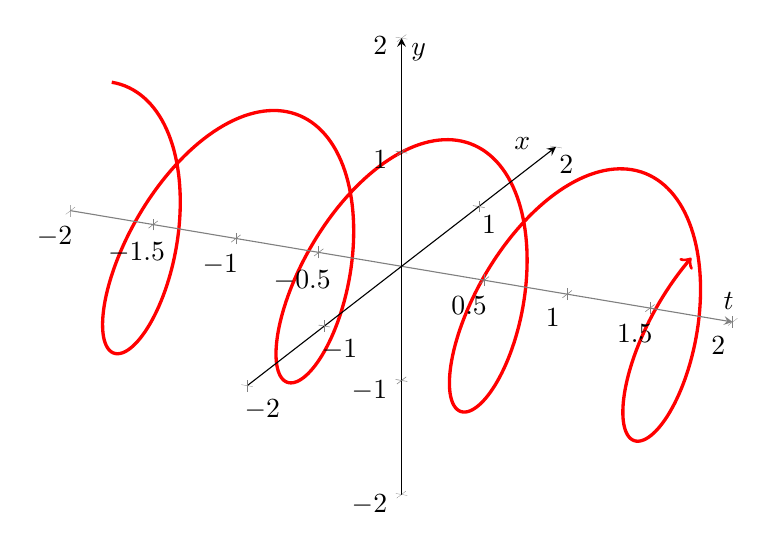
\begin{tikzpicture}[scale=1]\pgfplotsset{compat=1.8}
                \begin{axis}[enlargelimits=true,axis lines=center, axis on top, xlabel={$t$}, ylabel={$x$}, zlabel={$y$}, x axis line style=gray, %axis equal,view={35}{340},,
                    ymin=-2,ymax=2,zmin=-2,zmax=2,xmin=-2,xmax=2, x post scale=1.8, y post scale=1.8,z post scale=1.8]
                    \addplot3[samples=500, very thick,red, domain = -2:2, samples y =0,->] ({x},{sin(6*deg(x))},{cos(6*deg(x))});
                \end{axis}
            \end{tikzpicture}
		\begin{tikzpicture}[scale=1]\pgfplotsset{compat=1.8}
			\begin{axis}[enlargelimits=true,axis lines=center, axis on top, xlabel={$t$}, ylabel={$x$}, zlabel={$y$}, axis equal,view={90}{0},
                            ymin=-2,ymax=2,zmin=-2,zmax=2,xmin=-2,xmax=2,]
                            \addplot3[samples=500, very thick,red, domain = -2:2, samples y =0,->] ({x},{sin(6*deg(x))},{cos(6*deg(x))});
			\end{axis}
		\end{tikzpicture}
	\end{center}
\sld{\vfill\pagebreak[5]}%%%%%%%%%%%%%%%
Traçons maintenant le graphe de $\Gamma_1=(\R, \phi_2 )$ où $\phi_2: t \mapsto ( \cos( (3t/2)^{3} + 3t/2 ),\sin( (3t/2)^{3} +3t/2 ))$:
		\begin{center}	
			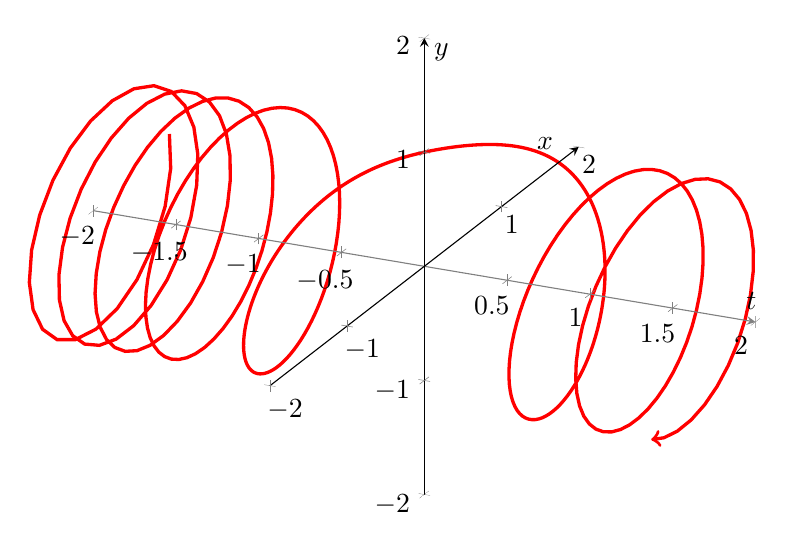
\begin{tikzpicture}[scale=1]\pgfplotsset{compat=1.8}
				\begin{axis}[enlargelimits=true,axis lines=center, axis on top, xlabel={$t$}, ylabel={$x$}, zlabel={$y$}, x axis line style=gray,%axis equal,view={35}{340},,
                                    ymin=-2,ymax=2,zmin=-2,zmax=2,xmin=-2,xmax=2,x post scale=1.8,y post scale=1.8,z post scale=1.8]
                                %\addplot3[samples=500, very thick,red, domain = -10.4:10.4, samples y =0] ({x*x*x/(8*8*8)},{sin(deg(x))},{cos(deg(x))});
                                \addplot3[samples=500, very thick,red, domain = -2:1.6, samples y =0,->] ({x},{sin(deg( (1.5*x)^3 +(1.5*x)) )},{cos( deg(((1.5*x)^3 + (1.5*x)) ))});
				\end{axis}
			\end{tikzpicture}
			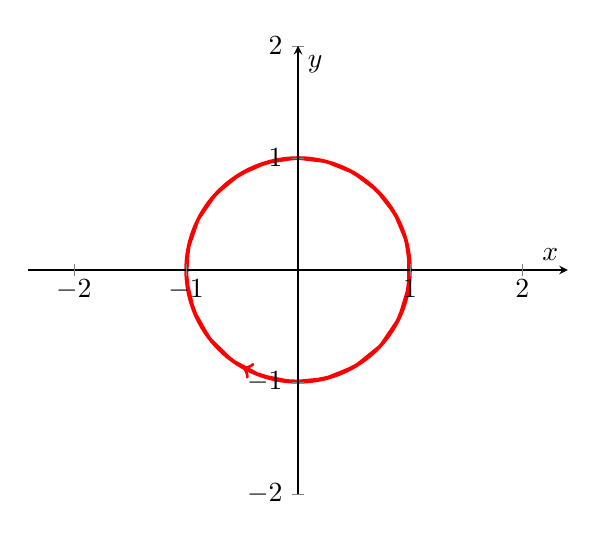
\begin{tikzpicture}[scale=1]\pgfplotsset{compat=1.8}
				\begin{axis}[enlargelimits=true,axis lines=center, axis on top, xlabel={$t$}, ylabel={$x$}, zlabel={$y$}, axis equal,view={90}{0},,
                                    ymin=-2,ymax=2,zmin=-2,zmax=2,xmin=-2,xmax=2]
                                \addplot3[samples=500, very thick,red, domain = -2:1.6, samples y =0,->] ({x},{sin(deg( (1.5*x)^3 +(1.5*x)) )},{cos( deg(((1.5*x)^3 + (1.5*x)) ))});
				\end{axis}
			\end{tikzpicture}
		\end{center}
		Les deux courbes $\Gamma_0$ et $\Gamma_1$ ont le même support et décrivent toutes deux le cercle unité du plan. Mais les vitesses de parcours sont différentes.
\end{exemple}

\begin{definition}
On dit qu'une courbe paramétrée $\Gamma=(I,\phi )$ de classe $\mathcal C^1$ est \emph{régulière} si pour tout $t\in I$ $\phi'(t) \neq 0$.
\end{definition}

\begin{remark}
Si $\Gamma_0 = (I,\phi)$ est une courbe paramétrée régulière et $\Gamma_1 = (J, \varphi =\phi \circ \theta)$ est une reparamétrisation admissible de $\Gamma_0$ alors $\Gamma_1$ est aussi régulière. En effet, comme $\theta: J \to I$ est une $\mathcal C^1$-difféomorphisme, on a:
            \[
                \forall t \in J, \varphi' (t) = \phi'(\theta(t)) \theta'(t) \neq 0.
            \]
\end{remark}

\begin{exemple}
    Considérons la courbe paramétrée définie par $\phi(t) = (t,t^2)$ pour $t\in\R$:
    %Une courbe paramétrée régulière admet une tangente en tout point (voir plus bas). La réciproque n'est pas vraie. 
            \begin{center}
                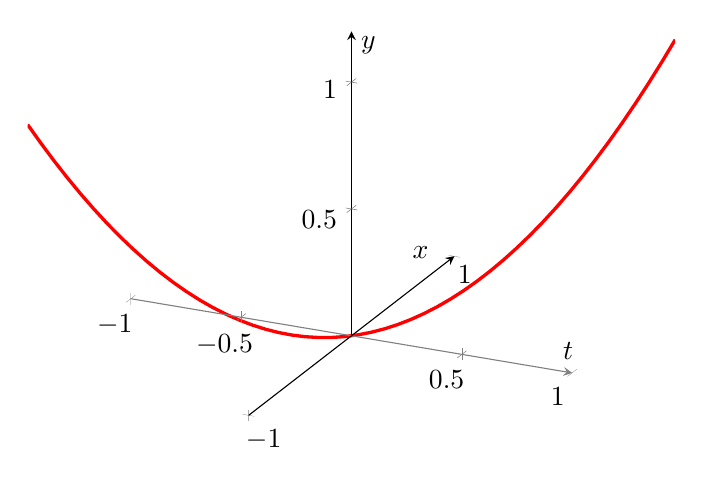
\begin{tikzpicture}[scale=1]\pgfplotsset{compat=1.8}
                    \begin{axis}[enlargelimits=true,axis lines=center, axis on top, xlabel={$t$}, ylabel={$x$}, zlabel={$y$}, x axis line style=gray, ymin=-1,ymax=1,zmin=0,zmax=1.2,xmin=-1,xmax=1,x post scale=1.2,y post scale=1.2,z post scale=1.2]
                    \addplot3[samples=50, very thick,red, domain =-1:1, samples y =0] ({x},{x},{x^2});
                    \end{axis}
                \end{tikzpicture}\hfill%
                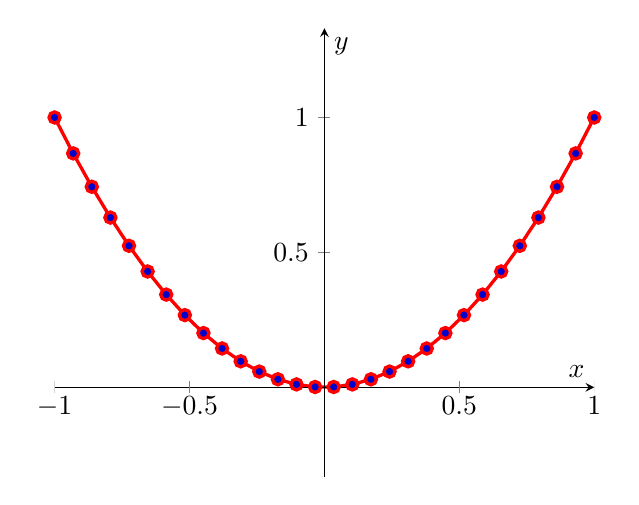
\begin{tikzpicture}[scale=1]\pgfplotsset{compat=1.8}
			\begin{axis}[enlargelimits=false,axis lines=center, axis on top, xlabel={$t$}, ylabel={$x$}, zlabel={$y$}, axis equal,view={90}{0},
                    ymin=-1,ymax=1,zmin=0,zmax=1,xmin=-.1,xmax=.1,%x post scale=1.8,y post scale=1.8,z post scale=1.8
                    ]
                        \addplot3+[samples=30, very thick,red, domain = -1:1, samples y =0] ({0},{x},{x^2});
			\end{axis}
		\end{tikzpicture}
            \end{center}
            La courbe paramétrée $\Gamma_1$ définie par $\phi_1(t)=(t^3 +t, (t^3 +t )^2)$ avec $t\in \R$ est une reparamétrisation admissible de $\Gamma$: 
            \begin{center}
                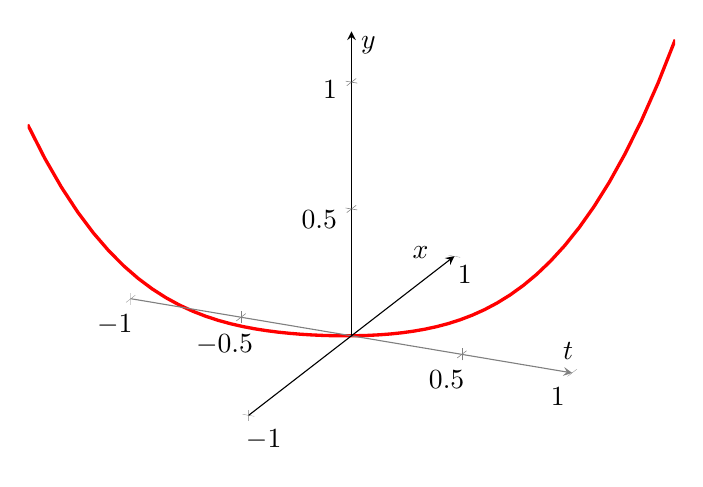
\begin{tikzpicture}[scale=1]\pgfplotsset{compat=1.8}
                    \begin{axis}[enlargelimits=true,axis lines=center, axis on top, xlabel={$t$}, ylabel={$x$}, zlabel={$y$}, x axis line style=gray, ymin=-1,ymax=1,zmin=0,zmax=1.2,xmin=-1,xmax=1,x post scale=1.2,y post scale=1.2,z post scale=1.2]
                        %\addplot3[samples=500, very thick,red, domain =-pi/4:pi/4, samples y =0] ({x},{tan(deg(x))},{(tan(deg(x)))^2});
                    \addplot3[samples=50, very thick,red, domain =-1:1, samples y =0] ({x},{(x^3 + x) /2},{((x^3 + x) /2)^2});
                    \end{axis}
                \end{tikzpicture}\hfill%
                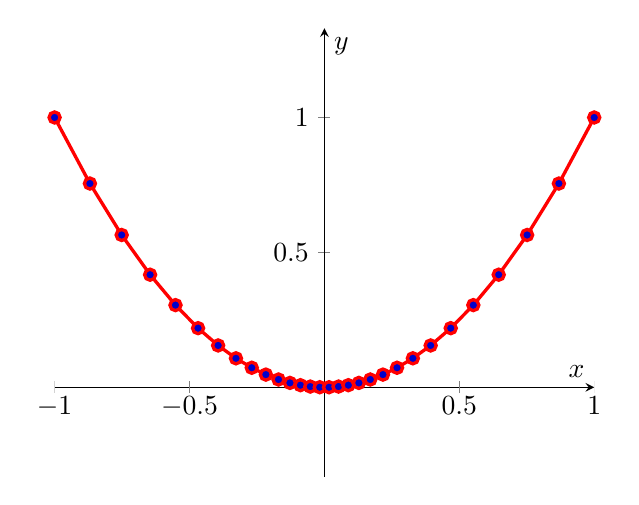
\begin{tikzpicture}[scale=1]\pgfplotsset{compat=1.8}
			\begin{axis}[enlargelimits=false,axis lines=center, axis on top, xlabel={$t$}, ylabel={$x$}, zlabel={$y$}, axis equal,view={90}{0},
                    ymin=-1,ymax=1,zmin=0,zmax=1,xmin=-.1,xmax=.1,%x post scale=1.8,y post scale=1.8,z post scale=1.8
                    ]
                        \addplot3+[samples=30, very thick,red, domain =-1:1, samples y =0] ({0},{(x^3 + x) /2},{((x^3 + x) /2)^2});
			\end{axis}
		\end{tikzpicture}
            \end{center}
    
La courbe paramétrée $\Gamma_2$ définie par $\phi_2(t)=(t^3,t^6)$ avec $t\in \R$ n'est pas une reparamétrisation admissible de $\Gamma$: 
            \begin{center}
                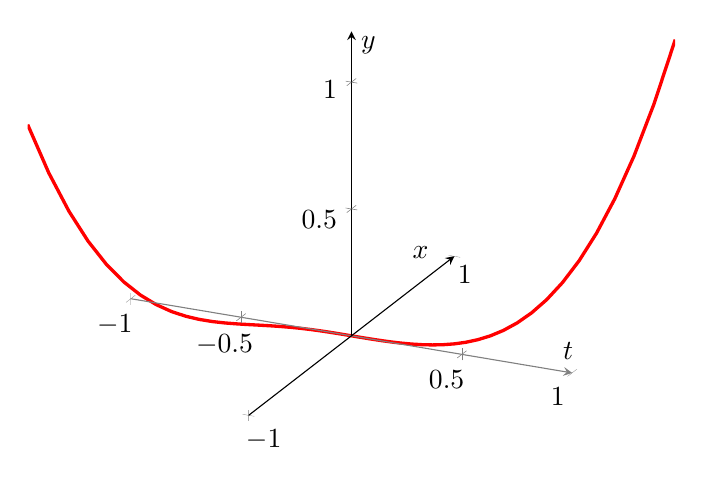
\begin{tikzpicture}[scale=1]\pgfplotsset{compat=1.8}
                    \begin{axis}[enlargelimits=true,axis lines=center, axis on top, xlabel={$t$}, ylabel={$x$}, zlabel={$y$}, x axis line style=gray, ymin=-1,ymax=1,zmin=0,zmax=1.2,xmin=-1,xmax=1,x post scale=1.2,y post scale=1.2,z post scale=1.2]
                    \addplot3[samples=50, very thick,red, domain =-1:1, samples y =0] ({x},{x^3},{x^6});
                    \end{axis}
                \end{tikzpicture}\hfill%
                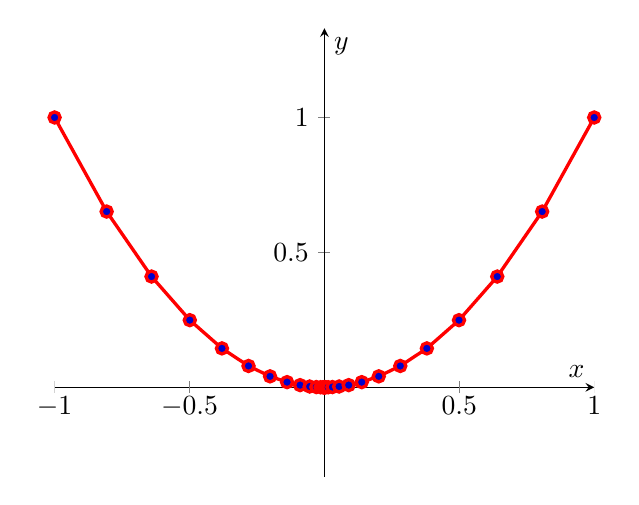
\begin{tikzpicture}[scale=1]\pgfplotsset{compat=1.8}
			\begin{axis}[enlargelimits=false,axis lines=center, axis on top, xlabel={$t$}, ylabel={$x$}, zlabel={$y$}, axis equal,view={90}{0},
                    ymin=-1,ymax=1,zmin=0,zmax=1,xmin=-.1,xmax=.1,%x post scale=1.8,y post scale=1.8,z post scale=1.8
                    ]
                        \addplot3+[samples=30, very thick,red, domain = -1:1, samples y =0] ({0},{x^3},{x^6});
			\end{axis}
		\end{tikzpicture}
            \end{center}
            La courbe géométrique associée est toujours la parabole d'équation $y=x^2$ mais on a ``créé un arrêt'' car $ \phi_3'(0)$ est nul. 
    \end{exemple}

\sld{\vfill\pagebreak[5]}%%%%%%%%%%%%%%%
\section{\'Etude locale d'un arc}

Soit $\Gamma=(I,\phi)$ une courbe paramétrée de classe $\Cc^k$, $k\in\N^*$ suffisamment grand. La formule de Taylor-Young en $t_0\in I$ s'écrit 
\[
	\phi(t_0 + h) =  \phi(t_0) + h \phi'(t_0) + \frac{h^2}{2} \phi''(t_0) + \cdots + \frac{h^k}{k!} \phi^{(k)}(t_0) + \sabs{h}^k \varepsilon(h). 
\]
où $\varepsilon: \R \to E$ satisfait $\lim_{h\to 0} \varepsilon(h) =0$. Si les vecteurs dérivées de $\phi$ ne sont pas tous nul en $t_0$, on note:  %existe $i\in \N^*$ tel que $\phi^{(i)}(t_0)\neq 0$, on note 

\begin{enumerate}
	\item $p$ le plus petit entier non nul tel que $\phi^{(p)}(t_0)\neq 0 $.
	\item  $q$ le premier entier supérieur à $p$ tel que $\phi^{(q)}(t_0)$ ne soit pas colinéaire à $\phi^{(p)}(t_0) $. Autrement dit, pour tout entier $i\in\left\{ p,\cdots,q-1\right\}$, il existe $\lambda_i\in\R$ tel que: $\phi^{(i)}(t_0) = \lambda_i \phi^{(p)} (t_0)$. 
\end{enumerate}\sld{\vfill\pagebreak[5]}%%%%%%%%%%%%%%%
La formule de Taylor-Young devient:
\[
	\phi(t_0 + h) =  \phi(t_0) + \left( \sum_{i=p}^{q-1} \lambda_i \frac{h^i}{i!} \right) \phi^{(p)}(t_0) + \frac{h^q}{q!} \phi^{(q)}(t_0)+ \sabs{h}^q \varepsilon(h).
\]
où $\varepsilon: \R \to E$ est tel que $\lim_{h\to 0} \varepsilon(h) =0$.

\begin{definition}
	Le point $\phi(t_0)$ est un point:
	\begin{enumerate}
		\item \emph{régulier} si $\phi'(t_0) \neq 0$ (cas $p=1$). 
		\item \emph{stationnaire} si $\phi'(t_0) =0$ (cas $p>1$). 
	\item \emph{birégulier} si $\phi'(t_0)$ et $ \phi''(t_0)$ ne sont pas colinéaires  ($p=1$ et  $q=2 $).
	\end{enumerate}
\end{definition}

\begin{definition}
	La \emph{tangente} à l'arc $\Gamma$ au point $M_0 = \phi(t_0)$ est la droite affine passant par $M_0$ et dirigée par le vecteur $\phi^{(p)}(t_0)$.
\end{definition}
 \pl{\rep{3cm}}

\begin{remark}
	L'entier $p$ et la droite tangente $\R\phi^{(p)}(t_0)$ sont invariant par changement de paramétrisation admissible.
\end{remark}

\begin{exemple}
	Retour sur $E =\R^3$ et $\phi: t \mapsto \left( \cos t, \sin t , \sinh t \right) \frac{1}{\cosh t} $ pour tout $t\in\R$. On montre que $\prs{\phi(t),\phi'(t)} = 0$ pour tout $t\in\R$.
	\pl{\rep{5cm}}
\end{exemple}
\sld{\vfill\pagebreak[5]}%%%%%%%%%%%%%%%
\begin{defprop}
	On se place dans le cas $E=\R^2$. On pose $M_0=\phi(t_0)$, les vecteurs $v = \phi^{(p)}(t_0) $ et $w = \phi^{(q)}(t_0)$  forment un base de $\R^2$ et $(M_0,v,w)$ est un repère du plan.
\begin{enumerate}
\item Cas $p$ impair et $q$ pair: point \emph{ordinaire}.
	\begin{center}
		\input{../chap_courbes/figures/fig_courbes_part3_06.tex}
	\end{center}
\item Cas $p$ impair et $q$ impair: point \emph{d'inflexion}.
	\begin{center}
		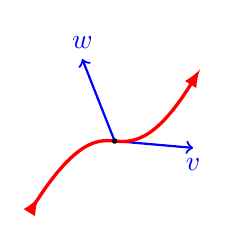
\begin{tikzpicture}[scale=1]

\begin{scope}[rotate=-5] 

  \draw[->,thick, blue] (0,0)--(1,0) node[below] {${v}$}; 
  \draw[->,thick, blue] (0,0)--(-0.5,1) node[above] {${w}$}; 
  \draw [>->,>=latex,very thick, color=red] (-1,-1) .. controls (-0.5,0) and (-0.2,0) .. (0,0) .. controls (0.2,0) and (0.5,0) .. (1,1);
 \fill (0,0) circle (1pt);
\end{scope}
\end{tikzpicture}

	\end{center}\sld{\vfill\pagebreak[5]}%%%%%%%%%%%%%%%
\item Cas $p$ pair et $q$ impair: point \emph{rebroussement de première espèce}.
	\begin{center}
		\input{../chap_courbes/figures/fig_courbes_part3_08.tex}
	\end{center}
\item Cas $p$ pair et $q$ pair: point \emph{rebroussement de deuxième espèce}.
	\begin{center}
		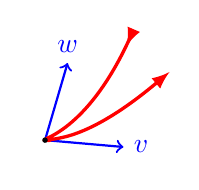
\begin{tikzpicture}[scale=1]

\begin{scope}[rotate=-5] 

  \draw[->, thick, blue] (0,0)--(1,0) node[right] {${v}$}; 
  \draw[->, thick, blue] (0,0)--(0.2,1) node[above] {${w}$}; 
  \draw [>->,>=latex,very thick, color=red] (1,1.5) .. controls (0.5,0) and (-0.2,0) .. (0.05,0.0) .. controls (0.1,0.05) and (0.5,0) .. (1.5,1);
 \fill (0,0) circle (1pt);
\end{scope}
\end{tikzpicture}

	\end{center}
\end{enumerate}
\end{defprop}

\pl{\rep{6cm}}
\sld{\vfill\pagebreak[5]}%%%%%%%%%%%%%%%

\section{\'Etude globale d'un arc paramétré - Cas plan ($E=\R^2$)}


\subsection{Branches infinies}

Soit $\Gamma=(I,\phi)$ un arc paramétré du plan $\R^2$ muni de la base canonique $(i,j)$. Pour $t\in I$, on pose $\phi(t) = (x(t),y(t))$ et $\snorm{\phi} = \sqrt{x^2(t) + y^2(t)}$. Dans ce qui suit, $a$ désigne une borne de $I$ (éventuellement infinie).

\begin{definition}
	On dit que $\Gamma$ admet une \emph{branche infinie} lorsque $t\to a$ si $\lim_{t\to a} \snorm{\phi(t)} = +\infty$
\end{definition}
\sld{\vfill\pagebreak[5]}%%%%%%%%%%%%%%%

Plusieurs cas se présentent 
\begin{enumerate}
	\item Si $\lim_{t\to a} \abs{x(t)} = +\infty$ et  $\lim_{t\to a} \abs{y(t)} = y_0$, alors la courbe $\Gamma$ admet la droite horizontale d'équation $y=y_0$ pour \emph{asymptote}.
		\begin{center}
			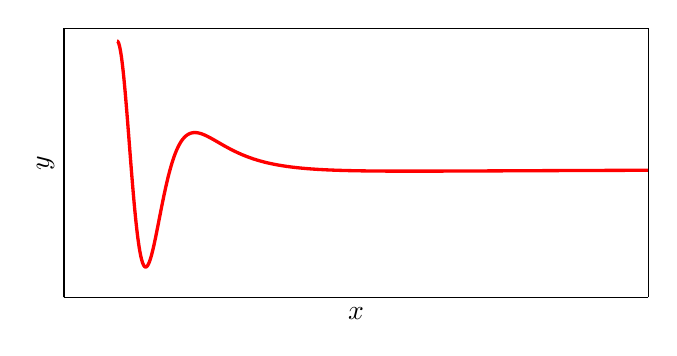
\begin{tikzpicture}
				\begin{axis}[xlabel = $x$,ylabel=$y$,zlabel=$z$,height=5cm,width=9cm,view={0}{90},, xmin=-1,xmax=10,ymin=-1,ymax=1.1,zmin=-0,zmax=0,xtick=\empty, ytick=\empty,]
					\addplot3[samples=500, very thick,red, domain = -0:pi/2, samples y =0] ({ tan(deg(x)) },{ (cos(deg(x)))^2 * cos(deg(6*x)) },{0});%CUBIQUE D'AGNESI
				\end{axis}
			\end{tikzpicture}
		\end{center}\sld{\vfill\pagebreak[5]}%%%%%%%%%%%%%%%

	\item Si $\lim_{t\to a} \abs{x(t)} = x_0$ et  $\lim_{t\to a} \abs{y(t)} = +\infty$, alors la courbe $\Gamma$ admet la droite verticale d'équation $x=x_0$ pour \emph{asymptote}.
		\begin{center}
			\begin{tikzpicture}
				\begin{axis}[xlabel = $x$,ylabel=$y$,zlabel=$z$,height=5cm,,view={0}{90},xmin=-2,xmax=4,ymin=-1,ymax=8,zmin=-0,zmax=0,xtick=\empty, ytick=\empty,
					]
					\addplot3[samples=500, very thick,red, domain = 0:10, samples y =0] ({ x^2 /(1+x^2) },{ x^3/(1+x^2)},{0});%CISSOÏDE DE DIOCLÈS
				\end{axis}
			\end{tikzpicture}
		\end{center}\sld{\vfill\pagebreak[5]}%%%%%%%%%%%%%%%

	\item On suppose que $\lim_{t\to a} \abs{x(t)} = +\infty$ et  $\lim_{t\to a} \abs{y(t)} = +\infty$, alors 
		\begin{enumerate}
			\item Si $\lim_{t\to a} \frac{y(t)}{x(t)} = 0$, on dit que $\Gamma$ admet une branche parabolique de direction $\R i$.
		\begin{center}
			\begin{tikzpicture}
				\begin{axis}[xlabel = $x$,ylabel=$y$,zlabel=$z$,height=6cm,width=10cm,view={0}{90},, xmin=-1,xmax=10,ymin=-1,ymax=5,zmin=-0,zmax=0,xtick=\empty, ytick=\empty,
					]
					\addplot3[samples=500, very thick,red, domain = -0:10, samples y =0] ({ (x+ 0*sin(deg(12*x)) )^2   },{ x+ ( x^2 /(1+x^2))*.6*sin(deg(6*x)) },{0});%CISSOÏDE DE DIOCLÈS
				\end{axis}
			\end{tikzpicture}
		\end{center}
			\item Si $\lim_{t\to a} \frac{y(t)}{x(t)} = \pm \infty$, on dit que $\Gamma$ admet une branche parabolique de direction $\R j$.\sld{\vfill\pagebreak[5]}%%%%%%%%%%%%%%%

			\item Si $\lim_{t\to a} \frac{y(t)}{x(t)} = \alpha$, deux cas se présentent
				\begin{enumerate}
					\item  Si $\lim_{t\to a} y(t) - \alpha x(t) =  \pm \infty$, on dit que $\Gamma$ admet une branche parabolique de direction $\R (i + \alpha j)$.
                                        \item  Si $\lim_{t\to a} y(t) - \alpha x(t) =  \beta$, on dit que $\Gamma$ admet la droite d'équation $y = \alpha x + \beta$ pour asymptote. Dans ce cas, on étudie la position de la courbe $\Gamma$ par rapport à l'asymptote. Pour cela, on étudie le signe de  $(y(t) - \alpha x(t) - \beta)$ au voisinage de $a$.
	\begin{center}
			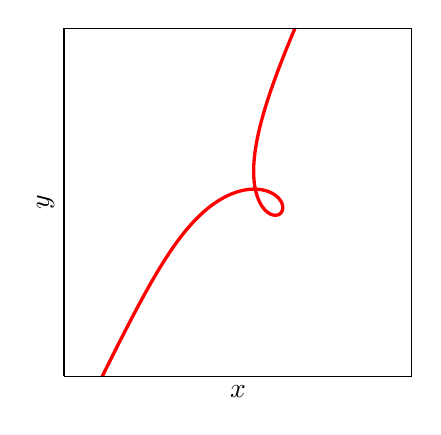
\begin{tikzpicture}
				\begin{axis}[xlabel = $x$,ylabel=$y$,zlabel=$z$,height=6cm,width=6cm,view={0}{90},, xmin=-8,xmax=8,ymin=-8,ymax=8,zmin=-0,zmax=0,xtick=\empty, ytick=\empty,
					]
					\addplot3[samples=500, very thick,red, domain = -10:10, samples y =0] ({2*(1-x^2)/(1+x^2) -x },{ 2*x * (1-x^2)/(1+x^2)  },{0});%CISSOÏDE DE DIOCLÈS
				\end{axis}
			\end{tikzpicture}
		\end{center}
				\end{enumerate}
		\end{enumerate}
\end{enumerate}

\sld{\vfill\pagebreak[5]}%%%%%%%%%%%%%%%

\section{Longueur et abscisse curviligne}

\begin{definition}
	Soit une courbe $\Gamma$ paramétrée par $\phi:[a,b] \to E$ de classe $\Cc^1$. La \emph{longueur} de $\Gamma$ est le nombre réel  
	\[
		L = \int_a^b \snorm{\phi'(t)}dt.
	\] 
La longueur est indépendante du choix de la paramétrisation.
\end{definition}

\begin{remark}
%	Soit $\Gamma$ un arc de $E$ paramétré par $\phi:[a,b] \to E$ continue mais non nécessairement $\Cc^1$:  
	On définit généralement la longueur d'une courbe paramétrée $\Gamma$ comme suit~: si l'ensemble des longueurs $L_\sigma>0$ des lignes polygonales inscrites dans $\Gamma$ où $\sigma$ décrit les subdivisions de $[a,b]$ admet une borne supérieure $L = \sum_{\sigma} L_{\sigma}$, on dit que l'arc $\Gamma$ est \emph{rectifiable} (noter que l'ensemble des courbes rectifiables est plus grand que l'ensemble des courbes $\Cc^1$). Le réel $L$ est appelé \emph{longueur} de $\Gamma$. Les deux définitions coïncident dans le cas des courbes $\Cc^1$.
	%\begin{center}
		%\begin{tikzpicture}
			%\draw[id=gamma] (0,0) edge[out=45, in= 135,] node[pos=.2] (bb){} node[pos=.4] (cc){} node[pos=.6] (dd){}   node[pos=.8] (ee){}  (3,2);

%\coordinate (a) at (0,0) ;
%\coordinate (b) at (1,1) ;
%\coordinate (c) at (2,1.5) ;
%\coordinate (d) at (3,2) ;
%\coordinate (e) at (4,1.2) ;

%%\draw[smooth] (a) to[out=50]  (b) to (c) to (d) to (e) ;
%%\draw[] (a) -- (b) -- (c) --(d) -- (e) ;


%\draw[] (a) -- (bb) -- (cc) -- (dd)-- (d);
		%\end{tikzpicture}
	%\end{center}
\end{remark}

\begin{exemple}
	Calcul de la longueur de l'ellipse paramétrée par $(x(t),y(t)) = (2\cos t,\sin t)$.
 \pl{\rep{4cm}}
\end{exemple}

\begin{definition}
	[(Abscisse curviligne)]
	Soit $\Gamma=(I,\phi)$ un arc paramétré de classe $\Cc^1$. Au réel $t_0$ correspond la fonction
	\begin{align*}
		s: I &\to \R\\
		t & \mapsto \int_{t_0}^t \snorm{\phi'(u)} du.
	\end{align*}
	appelée \emph{abscisse curviligne} d'origine $\phi(t_0)$ sur l'arc $\Gamma$ orienté dans le sens des $t$ croissants.
\end{definition}

\begin{exemple}
	Dans $\R^3$, on considère l'arc $\Gamma: t \mapsto \left( \cos t, \sin t , \sinh t \right) \frac{1}{\cosh t}$ défini sur $I=\R$.
 \pl{\rep{10cm}}
\end{exemple}

\begin{proposition}
	Soit $\Gamma=(I,\phi)$ un arc paramétré régulier de classe $\Cc^1$. L'abscisse curviligne sur $\Gamma$ permet de définir un nouveau paramétrage admissible de cet arc.
\end{proposition}

\begin{proof}
 \pl{\rep{6cm}}	
\end{proof}

{\bf \sffamily Interprétation cinématique:}  paramétrer par l'abscisse curviligne c'est parcourir le support de $\Gamma$ à vitesse constante 1.

\section{Plan d'étude}
Voici comment peut s'organiser l'étude d'une courbe paramétrée $\Gamma=(I,\phi)$. On suppose ici que $\phi$ est dans $\R^2$ (c'est donc une courbe du plan) et on note $t\mapsto x(t)$ et $t\mapsto y(t)$ les fonctions coordonnées.

\begin{description}
\item \emph{Domaine de définition de la courbe.}

La position du point $\phi(t)$ est défini si et seulement si ses coordonnées $x(t)$ et $y(t)$ sont définies.
Il faut ensuite déterminer un \emph{domaine d'étude} (plus petit que le domaine de définition) 
grâce aux symétries, périodicités\ldots 

\item \emph{Vecteur dérivé.} 

Calcul des dérivées des coordonnées de $t\mapsto \phi(t)$.
Les valeurs de $t$ pour lesquelles $x'(t)=0$ (et $y'(t)\neq0$) 
fournissent les points à tangente verticale et les valeurs de 
$t$ pour lesquelles $y'(t)=0$ (et $x'(t)\neq0$) fournissent les 
points à tangente horizontale. Enfin, les valeurs de $t$ pour 
lesquelles $x'(t)=y'(t)=0$ fournissent les points singuliers, 
en lesquels on n'a encore aucun renseignement sur la tangente.


\item \emph{Tableau de variations conjointes.} 

L'étude de $x'$ et $y'$ permet de connaître les variations de $x$ et $y$.
Reporter les résultats obtenus des \emph{variations conjointes} des fonctions $x$ et $y$
dans un tableau. Cela donne alors un tableau à compléter:

$$\begin{array}{|c|ccccc|}
\hline
t&\qquad&\qquad&\qquad&\qquad&\qquad\\
\hline
x'(t)& & & & &\rule{5cm}{0cm}\\
\hline
 & & & & & \\
x& & & & & \\
 & & & & & \\
\hline
 & & & & & \\
y& & & & & \\
 & & & & & \\
\hline
y'(t)& & & & & \\
\hline
\end{array}
$$

Ce tableau est le tableau des variations des
deux fonctions $x$ et $y$ \emph{ensemble}. Il nous montre 
l'évolution du point $\phi(t)$. 
%Par suite, pour une valeur de $t$ donnée, on doit lire 
%verticalement des résultats concernant et $x$, et $y$. Par 
%exemple, $x$ tend vers $+\infty$, pendant que $y$ ``vaut'' $3$.


\item \emph{\'Etude des points singuliers.} 

    À l'aide de la partie précédente, on peut facilement déterminer les points stationnaires (les temps $t$ où l'on a $x'(t)=y'(t)=0$). On peut alors étudier le comportement local de la courbe en ces points (rebroussement, inflexion, \textit{etc}\ldots). 

\item \emph{\'Etude des branches infinies.}

\item \emph{Construction méticuleuse de la courbe.}

On 
place dans l'ordre les deux axes et les unités. On construit 
ensuite toutes les droites asymptotes. On place ensuite les points 
importants avec leur tangente (points à tangente verticale, 
horizontale, points singuliers, points d'intersection 
avec une droite asymptote,\ldots).Tout est alors en place 
pour la construction.% et on peut tracer l'arc grâce aux règles suivantes:


%\mybox{
%\begin{tabular}{c}
%\textbf{Tracé de la courbe paramétrée $\big( x(t),y(t) \big)$}\\[2mm]
%Si $x$ croît et $y$ croît, on va vers la droite et vers le haut.\\
%Si $x$ croît et $y$ décroît, on va vers la droite et vers le bas.\\
%Si $x$ décroît et $y$ croît, on va vers la gauche et vers le haut.\\
%Si $x$ décroît et $y$ décroît, on va vers la gauche et vers le bas.
%\end{tabular}
%}




\item \emph{Points multiples.}

On cherche les points multiples s'il y a lieu. 
On attend souvent de commencer la construction de la courbe pour 
voir s'il y a des points multiples et si on doit les chercher.
\end{description}


%\addtocounter{chapter}{2}\chapter[Normes]{Normes sur $\R^n$ et limites}
% Source: chapitre 1 du Nigio: Fonction de plusieurs variables
% ref/normes/evn.pdf
%
% To do: ajouter les compacts ? caractérisation séquentielle des fermés ?

\sld{\vfill\pagebreak[5]}%%%%%%%%%%%%%%%

\section{Normes et distances}
Le but de se chapitre est de formaliser et de donner un sens précis à l'assertion ``$x$ est proche de $y$'' quand $x,y\in \R^n$. On sait déjà mesurer les distances dans $\R^n$. Si $A=\begin{psmallmatrix}
    x_1\\\vdots\\x_n
\end{psmallmatrix}$ et $B=\begin{psmallmatrix}
    y_1\\\vdots\\y_n
\end{psmallmatrix}$
sont deux points de $\R^n$. La distance est différente suivant que l'on mesure la trajectoire
\begin{itemize}
    \item ``à vol d'oiseau'': c'est la distance $\ell^2$ ou euclidienne.
    \item ``taxi cab'': distance $\ell^1$ ou ``city norm''.
\end{itemize}

\sld{\vfill\pagebreak[5]}%%%%%%%%%%%%%%%

\subsection{Normes}

%Une norme est une fonctionnelle qui sert à mesurer des distances dans les espace vectoriels.

\begin{definition}
    Soit un \rev{} $E$. Une \emph{norme} est une application $N: E \to \R^+ = [0,\infty[$ qui vérifie les propriétés suivantes~:
            \begin{enumerate}
                \item Séparation: $\forall u \in E, N(u) \geq 0 \text{ et } N(u) = 0 \Leftrightarrow u=0$,
                \item 	Homogénéité: $\forall u \in E, \forall \lambda \in \R, N(\lambda u) = \abs{\lambda} N(u)$,
                \item  Inégalité triangulaire: $\forall (u,v) \in E^2, N(u+v) \leq N(u) + N(v)$.
            \end{enumerate}
        \end{definition}

        Dans la suite, on notera le plus souvent $N(\cdot) = \norm{\cdot}$. L'espace $E$ muni d'une norme $\norm{\cdot}$ est appelé un espace normé et est noté $(E,\ncd)$.
%Une norme est une fonctionnelle qui sert à mesurer la ``proximité'' de deux éléments de $E$. Plus précisément, le nombre $N(x-y)$ sera interprété comme la ``longueur'' (en fait la distance) du vecteur $x-y$. 


        \sld{\vfill\pagebreak[5]}%%%%%%%%%%%%%%%
        \begin{exemple}
            Si $E = \R^n$ et si $u = (x_1,\cdots,x_n)\in E$, on définit les normes usuelles suivantes~:
            \begin{enumerate}
                \item La norme 1 est $\norm{u}_1 = \abs{x_1} + \cdots + \abs{x_n} $
                    \pl{\rep{4cm} }
                \item La norme 2 est $\norm{u}_2 = \sqrt{x_1^2 + \cdots + x_n^2}$ dispose de propriétés particulières (norme euclidienne).
                \item La norme infinie est $\norm{u}_\infty = \max\{\abs{x_1},\cdots, \abs{x_n} \} $
                    \pl{\rep{4cm} }
            \end{enumerate}
        \end{exemple}

        \begin{proposition}
            Soit $(E,\ncd)$ un espace normé. On a pour tout $u,v\in E$
            \[
                \big\lvert\norm{u}- \norm{v}\big\rvert \leq \norm{u -v}.
            \]
        \end{proposition}
%\begin{remark}
%	On peut interpréter cette dernière propriété de la manière suivante: une norme est donc une application 1-Lipschitzienne et donc continue. Nous donnerons un sens précis à tout cela dans la suite, mais on peut dors et déjà comprendre 

%	Cette dernière inégalité nous apprend que si $x$ et $y$ sont proches au sens de la norme $N$ alors leur norme est proche (c'est à rapprocher du concept de continuité).
%\end{remark}
        \begin{proof}\sld{
%On a pour tout $u,v\in E$: $\norm{u} = \norm{u-v+v} \leq \norm{u-v} + \norm{v} $. Ainsi $\norm{u} - \norm{v} \leq \norm{u-v}$.
%	De même  $\norm{v} = \norm{v-u + u} \leq \norm{v-u} + \norm{u} $ et donc $ -\norm{u-v} \leq \norm{v} - \norm{u}$. Mis bout %à bout on a bien 
%	\[
%		-\norm{u-v} \leq \norm{u} - \norm{v} \leq \norm{u-v}.\qedhere
%	\]
            }
            \pl{\rep{6cm} }
        \end{proof}

        \sld{\vfill\pagebreak[5]}%%%%%%%%%%%%%%%
        \subsection{Distances}

        \begin{definition}
        %Soit un espace normé $\left( E, \ncd \right)$ et $a$ et $b$ deux points de $E$. On appelle distance de $a$ à $b$ (déduite de la norme $\ncd$) la quantité $d(a,b) = \norm{b-a}$.
            Soit $E$ un ensemble, une \emph{distance} est une application $d:E\times E \to [0,+\infty[$ telle que 
                    \begin{enumerate}
                        \item Symétrie: $\forall u,v \in E$ on a $d(u,v) = d(v,u)$
                        \item Séparabilité: $d(u,v) = 0$ si et seulement si $u=v$
                        \item Inégalité triangulaire: $\forall u,v,w\in E$ on a $d(u,w) \leq  d(u,v) + d(v,w)$
                    \end{enumerate}
                \end{definition}
                Un espace $E$ muni d'une distance $d$ est appelé espace métrique. On note $(E,d)$. Un espace normé est un espace métrique:

                \begin{proposition}
                    Si $(E,\ncd)$ est un espace normé. L'application $d:E\times E \to [0,+\infty[$ définie par $d(u,v) = \norm{u-v}$ est une distance sur $E$.
                        \end{proposition}
                        \begin{proof}
%	Laissé en exercice.
                            \pl{\rep{5cm}}
                        \end{proof}

                        \begin{remark}
                            Toutes les distances ne sont pas issues de normes: dans $E=\R$ on définit $d:\R\times \R \to \R$ par $d(x,y) = \operatorname{atan}(\abs{x-y})$. % atan est croissante et concave.
                            \pl{\rep{5cm}}
                        \end{remark}


                        \sld{\vfill\pagebreak[5]}%%%%%%%%%%%%%%%
                        \subsection{Boules ouvertes et fermées}

                        La notion de norme généralise la notion de valeur absolue dans $\R$ aux espaces vectoriels. La définition suivante généralise la notion d'intervalle ouvert et fermé dans $\R$ aux espaces vectoriels:  

                        \begin{definition}
                            Soit $(E,\ncd)$ un \rev{} normé, $a\in E$  et un nombre réel $r>0 $ fixé. L'ensemble 
                            \[
                            B_r(a) = \{ u \in E, \norm{u-a}<r \}\]  est appelé \emph{boule ouverte} de centre $a$ et de rayon $r$. L'ensemble \[\overline{B_r}(a) = \{ u \in E, \norm{u-a}\leq r \}\] est appelé \emph{boule fermée} de centre $a$ et de rayon $r$. 
                        \end{definition}

                        \sld{\vfill\pagebreak[5]}%%%%%%%%%%%%%%%
                        \begin{exemple}
                            Voici les boules unités fermées dans $E=\R^2$ pour:
                            \begin{center}
                                \begin{tabular}{ccc}
                                    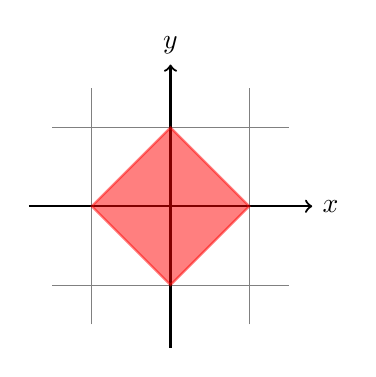
\begin{tikzpicture}
                                        \def\xone{-1.5};\def\xtwo{1.5};\def\yone{-1.5};\def\ytwo{1.5}

% grid
                                        \draw[step=1cm,help lines] (\xone,\yone) grid (\xtwo,\ytwo);
                                        \draw[thick,->] (\xone-.3, 0) -- (\xtwo+.3, 0) node[right] {$x$};
                                        \draw[thick,->] (0, \yone-.3) -- (0, \ytwo+.3) node[above] {$y$};
% ball
                                        \sld{	\draw[color=red,thick,fill=red, opacity=.5] (-1,0) -- (0,1) -- (1,0) -- (0,-1) -- cycle;}
                                    \end{tikzpicture}
                                    &
                                    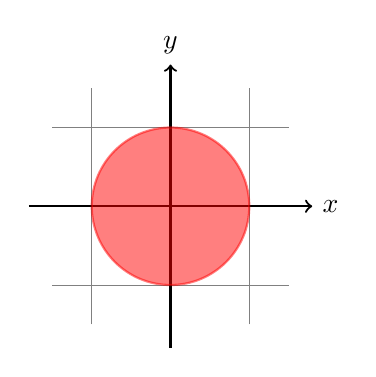
\begin{tikzpicture}
                                        \def\xone{-1.5};\def\xtwo{1.5};\def\yone{-1.5};\def\ytwo{1.5}
% grid
                                        \draw[step=1cm,help lines] (\xone,\yone) grid (\xtwo,\ytwo);
                                        \draw[thick,->] (\xone-.3, 0) -- (\xtwo+.3, 0) node[right] {$x$};
                                        \draw[thick,->] (0, \yone-.3) -- (0, \ytwo+.3) node[above] {$y$};
% ball
                                        \sld{
                                            \draw[color=red,thick,fill=red, opacity=.5] (0,0) circle (1cm);
                                        }
                                    \end{tikzpicture}&
                                    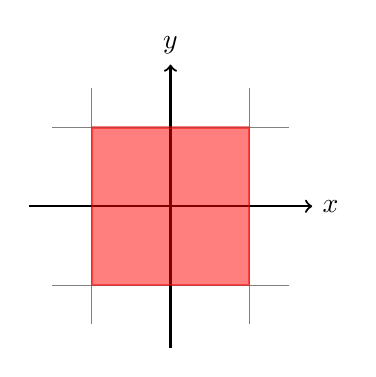
\begin{tikzpicture} 
                                        \def\xone{-1.5};\def\xtwo{1.5};\def\yone{-1.5};\def\ytwo{1.5};
% grid
                                        \draw[step=1cm,help lines] (\xone,\yone) grid (\xtwo,\ytwo);
                                        \draw[thick,->] (\xone-.3, 0) -- (\xtwo+.3, 0) node[right] {$x$};
                                        \draw[thick,->] (0, \yone-.3) -- (0, \ytwo+.3) node[above] {$y$};

% ball
                                        \sld{
                                            \draw[color=red,thick,fill=red, opacity=.5] (-1,-1) -- (-1,1) -- (1,1) -- (1,-1) -- cycle;
                                        }
                                    \end{tikzpicture}\\
                                    La norme $\ncd_1$
                                    & La norme $\ncd_2$
                                    & La norme $\ncd_\infty$
                                \end{tabular}
                            \end{center}
                        \end{exemple}

                        \sld{\vfill\pagebreak[5]}%%%%%%%%%%%%%%%
                        \begin{exemple}
                            Existe-t-il une norme dont la boule est l'un des ensembles suivants:
                            \begin{center}
                                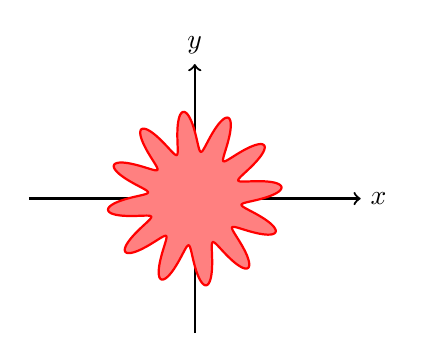
\begin{tikzpicture}
                                    \begin{axis}[height=3cm,xlabel = $x$,ylabel=$y$,height=5cm, axis equal,axis lines=middle, axis line style={->,thick}, xmin=-2,xmax=2,ymin=-2,ymax=2,xtick=\empty, ytick=\empty,every axis x label/.style={at={(current axis.right of origin)},anchor=west},every axis y label/.style={at={(current axis.above origin)},anchor=south},]
                                        \addplot[red,fill=red!50,samples=500, thick, domain = -pi:pi] ({cos(deg(x))*(1+ 0.3*sin(deg(12*x)))}, {sin(deg(x))*(1+ 0.3*sin(deg(12*x)))});
                                    \end{axis}
                                \end{tikzpicture}
                                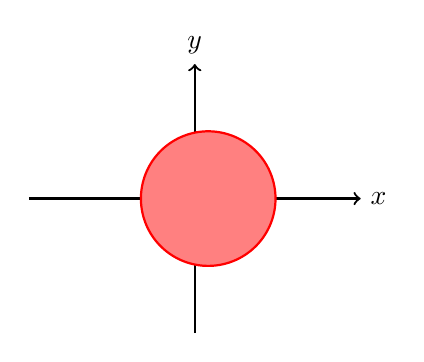
\begin{tikzpicture}
                                    \begin{axis}[height=3cm,xlabel = $x$,ylabel=$y$,height=5cm, axis equal,axis lines=middle, axis line style={->,thick}, xmin=-2,xmax=2,ymin=-2,ymax=2,xtick=\empty, ytick=\empty,every axis x label/.style={at={(current axis.right of origin)},anchor=west},every axis y label/.style={at={(current axis.above origin)},anchor=south},]
                                        \addplot[red,fill=red!50,samples=500, thick, domain = -pi:pi] ({cos(deg(x))+.2}, {sin(deg(x))});
                                    \end{axis}
                                \end{tikzpicture}
                                \begin{tikzpicture}
                                    \begin{axis}[height=3cm,xlabel = $x$,ylabel=$y$,height=5cm, axis equal,axis lines=middle, axis line style={->,thick}, xmin=-2,xmax=2,ymin=-2,ymax=2,xtick=\empty, ytick=\empty,every axis x label/.style={at={(current axis.right of origin)},anchor=west},every axis y label/.style={at={(current axis.above origin)},anchor=south},]
                                        \addplot[name path=F,red,domain={-3:3}] {1 +x};
                                        \addplot[name path=G,red,domain={-3:3}] {x-1};

                                        \addplot[red!50]fill between[of=F and G, soft clip={domain=-3:3}] ;

                                    \end{axis}
                                \end{tikzpicture}
                            \end{center}
                        \end{exemple}
                        \sld{\vfill\pagebreak[5]}%%%%%%%%%%%%%%%

                        \subsection{Normes équivalentes}

                        \begin{definition}[(Normes équivalentes)]
                            On dit que deux normes $\ncd$ et $\ncd': E\to\R$  sont équivalentes (et on note $\ncd \sim \ncd'$) s'il existe $\alpha>0$ et $\beta>0$ tels que, $\forall u \in E$
                            \[
                                \alpha \norm{u} \leq \norm{u}' \leq \beta \norm{u}
                            \]
                        \end{definition}

                        \begin{proposition}
                            La relation $\sim$ définit une relation d'équivalence sur les normes. 
                        \end{proposition}

                        \begin{proof}
                            \sld{
                %Soient $\ncd$, $\ncd'$ et $\ncd''$ trois normes sur $E$ alors la relation $\sim$ est~:
                %\begin{enumerate}
                        %\item Réflexive: on a $\ncd \sim \ncd$ en choisissant $\alpha = \beta =1$. 
                        %\item Symétrique: si $u\in E$ et $\alpha \norm{u} \leq \norm{u}' \leq \beta \norm{u}$ alors $\frac{1}{\beta} \norm{u}' \leq \norm{u} \leq \frac{1}{\alpha} \norm{u}'$.
                        %\item Transitive: si $u\in E$, $\alpha \norm{u} \leq \norm{u}' \leq \beta \norm{u} $  et $\alpha' \norm{u}' \leq \norm{u}'' \leq \beta' \norm{u}' $ alors $\alpha\alpha' \norm{u} \leq \norm{u}'' \leq \beta\beta' \norm{u} $.
                %\end{enumerate}
                            }
                            \pl{\rep{8cm}}
                        \end{proof}
                        \sld{\vfill\pagebreak[5]}%%%%%%%%%%%%%%%

                        \noindent On a l'interprétation géométrique suivante en termes de boules:
                        \begin{center}
                            \begin{tabular}{cc}
                                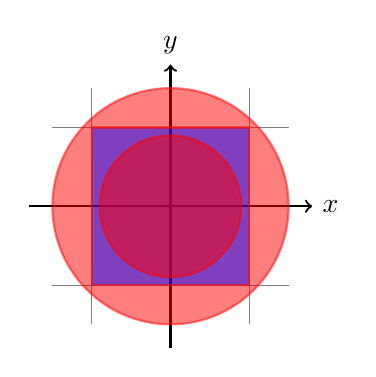
\begin{tikzpicture} 
                                    \def\xone{-1.5};\def\xtwo{1.5};\def\yone{-1.5};\def\ytwo{1.5};
% grid
                                    \draw[step=1cm,help lines] (\xone,\yone) grid (\xtwo,\ytwo);
                                    \draw[thick,->] (\xone-.3, 0) -- (\xtwo+.3, 0) node[right] {$x$};
                                    \draw[thick,->] (0, \yone-.3) -- (0, \ytwo+.3) node[above] {$y$};

% ball
                                    \draw[color=red,thick,fill=red,opacity=.5] (0,0) circle (1.5cm);
                                    \draw[color=red,thick,fill=blue,opacity=.5] (-1,-1) -- (-1,1) -- (1,1) -- (1,-1) -- cycle;
                                    \draw[color=red,thick,fill=red,opacity=.5] (0,0) circle (.9cm);

                                \end{tikzpicture} & 
                                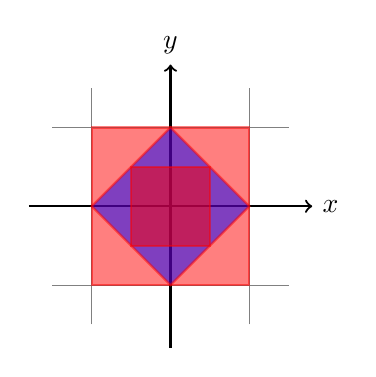
\begin{tikzpicture} 
                                    \def\xone{-1.5};\def\xtwo{1.5};\def\yone{-1.5};\def\ytwo{1.5};
% grid
                                    \draw[step=1cm,help lines] (\xone,\yone) grid (\xtwo,\ytwo);
                                    \draw[thick,->] (\xone-.3, 0) -- (\xtwo+.3, 0) node[right] {$x$};
                                    \draw[thick,->] (0, \yone-.3) -- (0, \ytwo+.3) node[above] {$y$};

% ball
                                    \draw[color=red,thick,fill=red,opacity=.5] (-1,-1) -- (-1,1) -- (1,1) -- (1,-1) -- cycle;
                                    \draw[color=red,thick,fill=blue,opacity=.5] (-1,0) -- (0,1) -- (1,0) -- (0,-1) -- cycle;
                                    \draw[color=red,thick,fill=red,opacity=.5] (-.5,-.5) -- (-.5,.5) -- (.5,.5) -- (.5,-.5) -- cycle;
                                \end{tikzpicture}
                                \\
                                $\ncd_2 \sim \ncd_\infty$
                                & $\ncd_\infty \sim \ncd_1$
                            \end{tabular}
                        \end{center}

                        \begin{theorem}
        %\label{}
                            Dans un \rev{} de dimension finie, toute les normes sont équivalentes.
                        \end{theorem}

                        \begin{proof}
                            Admis dans ce cours.
                        \end{proof}

                        \begin{remark}
                            Ce n'est pas vrai en dimension infinie. %Prendre $E = \mathcal C^1([0,1])$ avec $N_1$ et $N_\infty$.%mettre exemple C^1[0,1] du fichier /ref/normes/evn.pdf  page 5
                        \end{remark}

%\begin{proposition}
        %Les normes $N_1(\cdot),N_2(\cdot)$ et $N_\infty(\cdot)$ sont équivalentes sur $\R^n$.
%\end{proposition}

%\begin{proof}
%Il suffit de montrer que $N_\infty(x) \leq N_2(x) \leq N_1(x) \leq n N_\infty(x) $:
%\begin{itemize}
        %\item Tout d'abord:
                %\begin{align*}
                        %N_\infty(x) &= \left\{ \abs{x_1},\cdots,\abs{x_n} \right\} \\ 
                        %&= \sqrt{x_j^2} \qquad \text{(où $j$ est tel que $\abs{x_j} = N_\infty(x))$)}\\
                        %&= \sqrt{ x_1^2 + \cdots + x_n^2 } = N_2(x).
                %\end{align*}
        %\item \ldots puis:
%\begin{align*}			(N_2(x))^2 &= x_1^2 + \cdots+ x_n^2 \\ 
        %& \leq \abs{x_1}^2 + \cdots + \abs{x_n}^2 + 2 \sum_{1\leq i<j\leq n}\abs{x_i}\abs{x_j} \\ 
                        %&= ( \abs{x_1} + \cdots + \abs{x_n})^2 = (N_1(x))^2.
                %\end{align*}
        %\item \ldots et enfin
                %\begin{align*}
                        %N_1(x) &= \abs{x_1}+\cdots+\abs{x_n} \\
                        %& \leq n \max_{i=1,\ldots,n} \left\{ \abs{x_1},\cdots,\abs{x_n} \right\} \\
                        %& = n N_\infty(x).
                %\end{align*}
%\end{itemize}

%\end{proof}

                        \section{Limites de suites}

                        \begin{definition}[(Limite d'une suite)]
                            Soit $u=(u_k)_{k\in\N}$ une suite de points dans $(E,\ncd)$ et $\ell\in E$. On dit que la suite $u$ {converge} vers $\ell$ (ou la suite $u$ admet $\ell$ pour {limite}, ou $u$ tend vers $\ell$) au sens de la norme $\ncd$ si les conditions équivalentes suivantes sont satisfaites:
                            \begin{enumerate}
                                \item la suite de réels  $ \norm{u_{k} - \ell}$  tend vers 0 (\ie  $\lim_{k\to \infty} \norm{u_{k} -\ell} = 0$)
                                \item $\forall \varepsilon>0, \exists N\in\N, k\geq N \Rightarrow \norm{u_k - \ell} < \varepsilon$
                            \end{enumerate}
                        \end{definition}

                        \sld{\vfill\pagebreak[5]}%%%%%%%%%%%%%%%
                        \noindent Deux normes équivalentes ont les mêmes suites convergentes:
                        \begin{proposition}
                            Soit $E$ un \rev{} et $\ncd,\ncd': E \to [0,+\infty[$ deux normes équivalentes sur $E$. Pour toutes suites $(u_{k})_{k\in\N}$ et $\ell\in E$ les propriétés suivantes sont équivalentes:
                                    \begin{enumerate}
                                        \item $\lim_{k\to +\infty} u_{k} = \ell$ pour $\ncd$,
                                        \item $\lim_{k\to +\infty} u_{k} = \ell$ pour $\ncd'$.
                                    \end{enumerate}
                                \end{proposition}

                                \begin{proof}
                                    \pl{\rep{9cm}	}
                                \end{proof}

                                \sld{\vfill\pagebreak[5]}%%%%%%%%%%%%%%%
                                \noindent Dans $\R^n$ une suite converge si toutes les suites de ses coordonnées convergent:

                                \begin{proposition}
                                    Soit $u = (u_k)_{k\in\N} = \begin{psmallmatrix}u_{k,1}\\ \vdots \\ u_{k,n}\end{psmallmatrix}_{k\in\N}$ une suite de $\R^n$ et $\ell = \begin{psmallmatrix} \ell_1\\\vdots\\\ell_n\end{psmallmatrix} \in \R^n$. Alors les conditions suivantes sont équivalentes:
                                    \begin{enumerate}
                                        \item $\lim_{k\to +\infty} u_k = \ell$ dans $\R^n$
                                        \item Pour tout $i=1,\cdots,n$ on a  $\lim_{k\to +\infty} u_{k,i} = \ell_i$ dans $\R$
                                    \end{enumerate}
                                \end{proposition}

                                \begin{proof}
                                    \pl{\rep{8cm}	}

                                \end{proof}

                                \begin{remark}
                                    La limite est donc, si elle existe, unique.
                                \end{remark}

                                \sld{\vfill\pagebreak[5]}%%%%%%%%%%%%%%%
                                \section{Notions élémentaires de topologie}

                                \subsection{Ensembles ouverts et ensembles fermés}

                                \begin{definition}
                                    Soit $(E,\ncd)$ un \rev{} normé. On dit que 
                                    \begin{enumerate}
                                        \item une partie $\mathcal U$ de $E$ est un \emph{ouvert} pour la norme $\ncd$ si pour tout $a\in \mathcal U$, on peut trouver un réel $r>0$ tel que la boule $B_r(a) \subset \mathcal U$.  
                                        \item une partie $\mathcal F$ de $E$ est un \emph{fermé} pour la norme $\ncd$ si le complémentaire $E\setminus \mathcal F = \mathcal F^c = \left\{ u\in E| u \notin \mathcal F \right\}$ est une partie ouverte.
                                    \end{enumerate}
                                \end{definition}

                                \begin{exemple}
                                    \pl{\rep{5cm}	}
                                \end{exemple}

                                \sld{\vfill\pagebreak[5]}%%%%%%%%%%%%%%%
                                \begin{proposition}
                                Dans un \rev{} normé de dimension finie, une boule ouverte est un ouvert et une boule fermée est un fermé. \end{proposition}
                                \begin{proof}
                                    Soit $B_r(a)$ une boule ouverte de $\R^n$ et $x\in B_r(a)$. La boule $B_\rho(x)$ où $\rho = \frac{r - \norm{a -x}}{2}$ est incluse dans $B_r(a)$.
%\begin{center}
                                    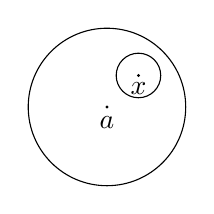
\begin{tikzpicture}
                                        \draw (0,0) node[below]{$a$} circle (0.01);
                                        \draw (0,0) circle (1cm);
                                        \draw (.4,.4) node[below=-1pt]{$x$} circle (0.01);
                                        \draw (.4,.4) circle (.2828);
                                    \end{tikzpicture}
%\end{center}
                                \end{proof}

                                \noindent Si deux normes sont équivalentes, alors les parties ouvertes (et fermées) sont les mêmes:
                                \begin{proposition}
                                    Soit $\mathcal U$ une partie d'un \rev{} $E$ et $\ncd$ et $\ncd'$ deux normes équivalentes sur $E$. La partie  $\mathcal U$ est un ouvert pour $\ncd$ si et seulement si $\mathcal U$ est un ouvert pour $\ncd'$.
                                \end{proposition}

                                \begin{proof}
                                    \pl{\rep{8cm}	}

                                \end{proof}


                                \begin{proposition}[(Caractérisation séquentielle des fermés)]
                                    Soit $\mathcal F$ une partie non vide d'un \rev{} normé $(E,\ncd)$. Les conditions suivantes sont équivalentes:
                                    \begin{enumerate}
                                        \item La partie $\mathcal F$ est fermée.
                                        \item Pour toute suite convergente de points de $\mathcal F$ alors la limite est dans $\mathcal F$.
                                    \end{enumerate}
                                \end{proposition}

                                \begin{proof}
                                    \pl{\rep{10cm}	}

                                \end{proof}

                                \sld{\vfill\pagebreak[5]}%%%%%%%%%%%%%%%
                                \subsection{Position d'un point}

                                \begin{definition}
                                    Soit $A$ une partie de $(E,\ncd)$ et $a\in E$. On dit que $a$ est un point
                                    \begin{enumerate}
                                        \item	\emph{Intérieur} à $A$ si on peut trouver un ouvert $\mathcal U \subset E$ tel que $a\in \mathcal U$ et $\mathcal U \subset A$. L'ensemble des points intérieurs à $A$ est noté $\mathring{A}$.
                                        \item	\emph{Adhérent} à $A$ si tout ouvert $\mathcal U \subset E$ qui contient $a$ satisfait $\mathcal U \cap A \neq \emptyset $. L'ensemble des points adhérents à $A$ est noté $\bar{A}$.
                                    \end{enumerate}
                                \end{definition}

                                \begin{center}
                                    \begin{tabular}{c}
                                        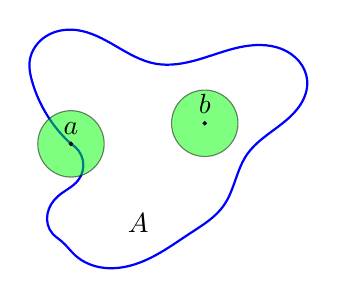
\begin{tikzpicture}[y=0.80pt, x=0.8pt,yscale=-1, scale=.3]
                                            \begin{scope}[]% layer1
  % path3029
                                                \path[,draw=blue,line join=miter,line cap=butt,line
                                                width=0.800pt] (98.5714,281.3729) .. controls (70.8127,256.1888) and
                                                (50.2769,223.1311) .. (40.0000,187.0872) .. controls (37.1535,177.1038) and
                                                (35.0669,166.6644) .. (36.4286,156.3729) .. controls (38.4655,140.9780) and
                                                (48.4007,127.1461) .. (61.6165,118.9916) .. controls (74.8322,110.8372) and
                                                (91.0080,108.1122) .. (106.4286,109.9443) .. controls (128.0218,112.5098) and
                                                (147.6221,123.3989) .. (166.4039,134.3576) .. controls (185.1857,145.3163) and
                                                (204.3205,156.7659) .. (225.7143,160.6586) .. controls (246.9864,164.5292) and
                                                (268.9327,160.5990) .. (289.7117,154.6226) .. controls (310.4907,148.6461) and
                                                (330.6998,140.6190) .. (351.8282,136.0281) .. controls (372.9566,131.4372) and
                                                (395.5974,130.4743) .. (415.6901,138.4597) .. controls (425.7365,142.4524) and
                                                (434.9733,148.6809) .. (441.9302,156.9558) .. controls (448.8871,165.2306) and
                                                (453.4851,175.5919) .. (454.2857,186.3729) .. controls (455.2115,198.8397) and
                                                (451.0656,211.3250) .. (444.3564,221.8733) .. controls (437.6472,232.4215) and
                                                (428.4885,241.2021) .. (418.7670,249.0615) .. controls (399.3239,264.7803) and
                                                (376.7905,277.7558) .. (362.8571,298.5157) .. controls (355.1132,310.0538) and
                                                (350.5022,323.3562) .. (345.9050,336.4696) .. controls (341.3077,349.5829) and
                                                (336.5511,362.8537) .. (328.5714,374.2300) .. controls (316.0601,392.0670) and
                                                (296.7907,403.7108) .. (278.5714,415.6586) .. controls (251.8717,433.1677) and
                                                (225.7667,452.6496) .. (195.4016,462.5190) .. controls (180.2191,467.4537) and
                                                (164.0573,469.8610) .. (148.1972,468.0391) .. controls (132.3371,466.2172) and
                                                (116.7890,459.9948) .. (105.0000,449.2300) .. controls (97.9078,442.7540) and
                                                (92.2774,434.7828) .. (85.0000,428.5157) .. controls (80.2575,424.4316) and
                                                (74.8328,421.0855) .. (70.7143,416.3729) .. controls (67.2344,412.3909) and
                                                (64.8038,407.5229) .. (63.5652,402.3817) .. controls (62.3267,397.2404) and
                                                (62.2694,391.8345) .. (63.2502,386.6379) .. controls (65.2118,376.2448) and
                                                (71.2992,366.8784) .. (79.2857,359.9443) .. controls (84.1039,355.7611) and
                                                (89.5750,352.4139) .. (94.8588,348.8368) .. controls (100.1426,345.2597) and
                                                (105.3244,341.3751) .. (109.2857,336.3729) .. controls (115.8694,328.0591) and
                                                (118.6048,316.8181) .. (116.5770,306.4089) .. controls (114.5492,295.9997) and
                                                (107.7944,286.6074) .. (98.5714,281.3729);

                                                \coordinate (a) at (98.5714,281.3729) ;
                                                \draw[fill=green,opacity=.5] (a)  circle (40pt);
                                                \draw[fill=blue,opacity=1] (a) node[above,opacity=1]{$a$}  circle (2pt);

                                                \coordinate (b) at (300,250.3729) ;
                                                \draw[fill=green,opacity=.5] (b)  circle (40pt);
                                                \draw[fill=blue,opacity=1] (b) node[above,opacity=1]{$b$}  circle (2pt);

                                                \node (A) at (200,400) {$A$};
                                            \end{scope}
                                        \end{tikzpicture}\\ 
                                        Le point $a$ est adhérent à $A$ et $b$ est intérieur à $A$.
                                    \end{tabular}
                                \end{center}

                                \begin{remark}
                                    La partie $\mathring{A}$ est ouverte et la partie $\bar A$ est fermée.
                                \end{remark}
                                \begin{exemple}
                                    \pl{\rep{9cm}	}
                                \end{exemple}

                                \sld{\vfill\pagebreak[5]}%%%%%%%%%%%%%%%
                                \subsection{Ensembles compacts}

                                \pl{Rappel sur les suites extraites\rep{5cm}}


                                \begin{definition}
                                    Une partie $\mathcal K$ d'un \rev{} $(E,\ncd)$ est dite \emph{compacte} si de toute suite de points de $\mathcal K$ on peut extraire une sous suite convergente dont la limite est dans $\mathcal K$.
                                \end{definition}
                                Autrement dit, toute suite de $\mathcal K$ admet une valeur d'adhérence dans $\mathcal K$.

                                \begin{theorem}
                                    [(Bolzano-Weierstrass)] Dans un \rev{} normé de dimension finie, les parties compactes sont les parties fermées bornées.
                                \end{theorem}

                                \begin{proof}
                                    Admise dans ce cours\ldots mais identique à la preuve dans le cas réel.
                                \end{proof}

                                \begin{exemple}
                                    \pl{\rep{3cm}	}
                                \end{exemple}

%\section{Limite d'une suite}

%\begin{definition}
        %Soit $\left( x_n \right)_{n\in\N}$ une suite de points de $\R^n$ et $\norm{\cdot}$ une norme. On dit que la suite $(x_n)$ a pour limite $\ell \in \R^n$ si 
        %$\forall \varepsilon >0, \exists n_0 \in \N$ ($n_0$ dépend de $\varepsilon$) tel que $n\geq n_0 \Rightarrow \norm{x_n - \ell } \leq \varepsilon$.
%\end{definition}

%Il existe des définitions équivalentes en termes de boules (ouvertes ou fermée) ou d'ouverts. Dans les espaces de dimension finie, la notion de limite et la limite elle même ne dépendent pas de la norme considérée. 

%\addtocounter{chapter}{3}\chapter{Espaces euclidiens}

\sld{\vfill\pagebreak[5]}%%%%%%%%%%%%%%%
\section{Formes Bilinéaires et formes quadratiques}

\subsection{Formes bilinéaires symétriques}

\begin{definition}
	Une \emph{forme bilinéaire} sur un $\R$ espace vectoriel $E$ est une application $\varphi: E\times E \to \R$ qui est linéaire par rapport à chacune de ses variables: 
	\begin{enumerate}
		\item  $\forall u,v,w\in E$ et $\lambda,\mu\in\R$, $\varphi(\lambda u + \mu v,w) = \lambda \varphi(u,w) + \mu \varphi(v,w)$,
		\item  $\forall u,v,w\in E$ et $\lambda,\mu\in\R$, $\varphi(u,\lambda v + \mu w) = \lambda \varphi(u,v) + \mu \varphi(u,w)$.
	\end{enumerate}
	Elle est \emph{symétrique} si $\varphi(u,v) = \varphi(v,u)$ pour tout $u,v\in E$
\end{definition}

\noindent \'Etant donnée une base $\mathcal B = \left( e_1,\cdots,e_n \right)$ de $E$ et $u=x_1 e_1 + \cdots+ x_n e_n$ et $v=y_1e_1+\cdots+y_n e_n$. On a 
\[
	\varphi (u,v) = \sum_{i=1}^n \sum_{j=1}^n m_{ij} x_iy_j
\]
$m_{ij} = \varphi(e_i,e_j) \in \R$ pour tout $i,j = 1,\cdots,n$. Ainsi une forme bilinéaire s'écrit comme comme un polynôme homogène de degré 2 en les coordonnées de $u$ et $v$.


\begin{exemple}
	\pl{\rep{7cm}}
\end{exemple}

\subsection{Formes quadratiques}

\begin{definition}
	Soit $E$ un $\R$ espace vectoriel. Une application $q:E \to \R$ est appelée une \emph{forme quadratique} s'il existe une forme bilinéaire $\varphi:E\times E \to \R$ telle que pour tout $u\in E$
	\[
q(u) = \varphi(u,u)
	\]
On dit que $\varphi$ est associée à $q$. ($q$ est un polynôme homogène de degré 2 en les coordonnées).
\end{definition}

\begin{exemple}
	\pl{\rep{3cm}} %norme euclidienne
\end{exemple}

\sld{\vfill\pagebreak[5]}%%%%%%%%%%%%%%%

%\noindent Lorque l'on écrit le vecteur $u$ dans une base, une forme quadratique est un polymôme homogène de degré 2 en les coordonnées de $u$.

\begin{proposition}
	Toute forme quadratique $q$ sur un \rev{} $E$ est associée à une unique forme bilinéaire symétrique.
\end{proposition}

\begin{proof}
		\pl{\rep{10cm}}
\end{proof}
\pl{\pagebreak[5]}
\begin{exemple}
Soit $q(x_1,x_2) = x_1^2 +x_2^2$.

\pl{\rep{6cm}} %norme euclidienne
\end{exemple}
\begin{definition}
	Soit $q:E\to\R$ une forme quadratique définie sur un \rev{} $E$. La forme bilinéaire symétrique $\varphi(u,v) = \frac{1}{4} \left( q(u+v) - q(u-v) \right)$ est la \emph{forme polaire} de $q$.
\end{definition}
\begin{exemple}
Soit $E=\R^3$ et  $q:(x_1,x_2,x_3) \mapsto 7x_1^2 +5  x_2 x_3$.

\pl{\rep{9cm}} %norme euclidienne
\end{exemple}

\sld{\vfill\pagebreak[5]}%%%%%%%%%%%%%%%

\subsection{Notation matricielle}

	Soit $E$ un \rev{} de dimension finie et $\mathcal B = (e_1,\cdots,e_n)$ une base de $E$ et $u=x_1 e_1 + \cdots+ x_n e_n$ et $v=y_1e_1+\cdots+y_n e_n$ deux éléments de $E$. Une forme bilinéaire symétrique sur $E$ s'écrit
	\[
		\varphi (u,v) = \sum_{i=1}^n \sum_{j=1}^n \underbrace{\varphi(e_i,e_j)}_{=m_{ij}} x_iy_j.
	\]
	Réciproquement si $(m_{ij})_{i,j=1}^n$ est une famille de réels telles que $m_{ij} = m_{ji}$ pour tout $i,j=1,\cdots,n$. Alors 
	\[
		(u,v) \mapsto \sum_{i=1}^n \sum_{j=1}^n m_{ij} x_i y_j
	\]
	est une forme bilinéaire symétrique sur $E$.

\sld{\vfill\pagebreak[5]}%%%%%%%%%%%%%%%

\begin{definition}
	Soit $E$ un \rev{} de dimension finie et $\mathcal B = (e_1,\cdots,e_n)$ une base de $E$. 
	\begin{enumerate}[label=$(\roman*)$]
		\item La matrice 
			\[\redspace 
				M = \left[ m_{ij}= \varphi(e_i,e_j) \right]_{i,j=1}^n
			\] 
			est appelée \emph{matrice de la forme bilinéaire symétrique} $\varphi$ dans la base $\mathcal B$.
		\item	La matrice (dans la base $\mathcal B$) de la forme quadratique $q(u) = \varphi(u,u)$ est la matrice $M$ de $\varphi$. Autrement dit, la matrice d'une forme quadratique est la matrice de sa forme polaire.
	\end{enumerate}
\end{definition}

Si $X = \begin{pmatrix}
	x_1\\\vdots\\x_n
\end{pmatrix}$ et $Y = \begin{pmatrix}
	y_1\\\vdots\\y_n
\end{pmatrix}$  sont les matrices colonnes des coordonnées de $u$ et $v$ dans la base $\mathcal B$, on a 
\[\redspace
	\varphi(u,v) = X^t M Y = Y^t M X = \varphi(v,u)
\]
et
\[\redspace
q(u) = X^t M X.
\]
On a de plus $M = M^t$.
\begin{exemple}
1) Soit $E=\R^2$ et $q(u) = x_1^2 + x_2^2$
	\pl{\rep{2cm}} %norme euclidienne
2) Soit $E=\R^3$ et  $q:(x_1,x_2,x_3) \mapsto 7x_1^2 + 6 x_1x_2 +  5  x_2 x_3$.

\pl{\rep{4cm}} %norme euclidienne
\end{exemple}


\sld{\vfill\pagebreak[5]}%%%%%%%%%%%%%%%

\section{Produit scalaire et norme euclidienne}

%Un produit scalaire est une fonctionnelle qui permet de mesurer des distances et des angles. C'est à dire, tout ce qu'il faut pour faire de la géométrie (au sens classique du terme du moins).


\subsection{Produit scalaire}

\begin{definition}
	On dit qu'une forme bilinéaire est 
	\begin{enumerate}[label=$(\roman*)$]
		\item \emph{Symétrique}: si $\forall u,v\in E, \varphi(u,v) = \varphi(v,u)$. 
		\item \emph{Positive}: si $\forall u\in E, \varphi(u,u) \geq 0$.
		\item \emph{Définie}: si $\varphi(u,u) =0 \Leftrightarrow u=0$. 
	\end{enumerate}
	Une forme forme bilinéaire symétrique définie positve est appelé \emph{produit scalaire}. 
\end{definition}

Suivant les auteurs et le contexte, le produit scalaire est noté $(u,v) \mapsto \prs{u,v}$ ou $(u,v) \mapsto \prs{u|v}$ ou encore $(u,v) \mapsto (u|v)$.

\begin{definition}
	Un espace euclidien est un espace vectoriel réel $E$ de dimension finie muni d'un produit scalaire $\prs{\cdot,\cdot}$. On note $(E,\prs{\cdot,\cdot})$.
\end{definition}

\begin{exemple}
	\plprof{1) Dans $E=\R^n$, l'application $\prs{(x_1,\cdots,x_n), (y_1,\cdots,y_n)} = x_1y_1 +\cdots + x_n y_n$ est le produit scalaire canonique. 

2) Dans $\R^2$ $\prs{(x_1,x_2),(y_1,y_2)} = (x_1 + x_2) (y_1+y_2) + 2 x_2y_2$ définit bien un produit scalaire.
	}
	\pl{\rep{5cm}} %norme euclidienne
\end{exemple}

\subsection{Norme euclidienne}

Soit l'application 
\begin{align*} 
	\norm{\cdot}: E &\to \R \\ u&\mapsto \norm{u} = \sqrt{\prs{u,u}}
\end{align*}
Remarquons qu'elle est bien définie car le produit scalaire est positif. %On note cette application comme une norme: c
%On s'intéresse maintenant aux propriétés de la fonction $E \times E \to \R $ défini par $(x,y) \to \sqrt{\prs{x,y}}$.
\begin{exemple}
	Si $E=\R$ on voit que la $\norm{\cdot}$ est simplement la valeur absolue. Si $E = \R^n$ avec le produit scalaire canonique alors $\norm{(x_1,\cdots,x_n)} = \sqrt{ x_1^2 + \cdots + x_n^2 }$.
\end{exemple}

\sld{\vfill\pagebreak[5]}%%%%%%%%%%%%%%%

\begin{proposition}
	[(Inégalité de Cauchy-Schwarz)] Pour tous $u,v \in E $ on a:
	\[
		%\abs{\prs{x,y}} \leq \sqrt{\prs{x,x}} \sqrt{\prs{y,y}}
		\abs{\prs{u,v}} \leq \norm{u} \norm{v}
	\]
	De plus on a $\abs{\prs{u,v}} = \norm{u} \norm{v} $ si et seulement si il existe un $\lambda\in\R$ tel que  $v=\lambda u$.
\end{proposition}

\begin{proof}\plprof{On considère plusieurs cas:
	\sld{	\begin{enumerate}
		\item 	Cas $u=0$ ou $v=0$: tout est facilement vérifiable et découle des propriétés du produit scalaire.
		\item 	Cas $u \neq 0$ et $v\neq 0$: tout d'abord, remarquer que l'on a pour tout $u\in E \setminus \{0\}$ on a 
			\[
				\prs{u,u} >0 \text{ et }\prs{ \frac{u}{{\norm{u}}},\frac{u}{{\norm{u}}} } = 1
			\]
			Cela implique que:
			\begin{equation*}\label{eq.cs1}
				0 \leq \norm{ \frac{u}{{\norm{u}}} + \frac{v}{{\norm{v}}} }^2  = 2 + 2 \frac{\prs{u,v}}{{\norm{u}}{\norm{v}} }
			\end{equation*}
			Ainsi, on en déduit que  $-{\norm{u}} {\norm{v}} \leq \prs{u,v} $. De même
			\begin{equation*}
				0 \leq \norm{ \frac{u}{{\norm{u}}} - \frac{v}{{\norm{v}}} }^2  = 2 - 2 \frac{\prs{u,v}}{{\norm{u}}{\norm{v}} }
			\end{equation*}
			Ainsi, on en déduit que $\abs{\prs{u,v}} \leq {\norm{u}} {\norm{v}} $. %On a donc $-\sqrt{\prs{x,x}} \sqrt{\prs{y,y}} \leq \prs{x,y} \leq \sqrt{\prs{x,x}} \sqrt{\prs{y,y}} $, 
			Cela termine la démonstration de l'inégalité. 

			Pour le cas d'égalité, on a $v=\lambda u$ pour $\lambda \in \R\setminus\{0\}$ si et seulement si $\norm{ \frac{v}{{\norm{u}}} + \frac{v}{{\norm{v}}} }^2 = 0$  ou $ \norm{ \frac{u}{{\norm{u}}} - \frac{v}{{\norm{v}}}} =0$ si et seulement si $ -\prs{u,v} = {\norm{u}} {\norm{v}}$ ou $ \prs{u,v} = {\norm{u}} \norm{v}$. 

	\end{enumerate}}}
	\pl{\rep{11cm}}
\end{proof}

\begin{remark}
	\begin{enumerate}
		\item On peut bien sûr utiliser l'expression (au carré): $\abs{\prs{u,v}}^2 \leq \prs{u,u}\prs{v,v}$
		\item Si $E=\R^n$ muni du produit scalaire cannonique, on obtient $(\sum_{i=1}^n x_iy_i)^2 \leq \sum_{i=1}^n x_i \sum_{i=1}^n y_i$
	\end{enumerate}
\end{remark}

\sld{\vfill\pagebreak[5]}%%%%%%%%%%%%%%%

\begin{proposition}[(Inégalité de Minkowski)]
$\forall u,v\in E$ on a 
\[
	{\norm{u+v}} \leq {\norm{u}} + {\norm{v}}.
\]
De plus on a $\norm{u+v} = \norm{u} + \norm{v} $ si et seulement si il existe un $\lambda\in\R$ tel que  $v=\lambda u$.
\end{proposition}
\begin{proof}\plprof{
	\sld{	C'est une conséquence de l'inégalité de Cauchy-Schwarz:
		\begin{align*}
			\norm{u+v}^2=\prs{u+v,u+v} &= \norm{u}^2 + \norm{v}^2 + 2\prs{u,v}\\
			& \leq \norm{u}^2 + \norm{v}^2 + 2\abs{\prs{u,v}} \\
			& \leq \norm{u}^2 + \norm{v}^2 + 2\prs{u,u}\prs{v,v} \\
			& \leq (\norm{u} + \norm{v})^2.
		\end{align*}}}
	\pl{\rep{5cm}}
\end{proof}


\noindent Un espace euclidien est en fait un espace normé:
\begin{defprop}
	Soit  un espace euclidien $(E,\prs{\cdot,\cdot})$. L'application $\norm{\cdot}: E \to \R $ définie pour tout $u\in E$ par $\norm{u} = \sqrt{\prs{u,u}}$ est une norme sur $E$ et elle est appelé \emph{norme euclidienne}.
\end{defprop}
\begin{proof} On vérifie les trois propriétés vérifiées pour une norme:
	\begin{enumerate}
		\item $\norm{u} = 0 \Rightarrow \prs{u,u}=0 \Rightarrow u=0 $ car le produit scalaire est défini. 
		\item homogénéité $\norm{\lambda u} = \sqrt{\prs{\lambda u, \lambda u}} = \sqrt{\lambda^2} \sqrt{\prs{u,u}} = \abs{\lambda} \norm{u}$.
		\item Inégalité triangulaire: c'est exactement l'inégalité de Minkowski.
	\end{enumerate}
\end{proof}

\noindent 	Les normes euclidiennes sont donc des normes bien particulières car elles découlent d'un produit scalaire. Les normes euclidiennes satisfont un certain nombre de propriétés remarquables:

\begin{proposition}
	Soit  un espace euclidien $(E,\prs{\cdot,\cdot})$ et $\norm{\cdot}$ la norme euclidienne sur $E$. Pour tous $u,v\in E$ on a
\begin{align*}
	\prs{u,v} = \frac{1}{2} \left( \norm{u+v}^2 - \norm{u}^2 - \norm{v}^2 \right) = \frac{1}{4}\left( \norm{u+v}^2 - \norm{u-v}^2 \right) 
	\intertext{ et  }
	\norm{u+v}^2 + \norm{u-v}^2 = 2\left( \norm{u}^2 + \norm{v}^2 \right)
\end{align*}
\end{proposition}

\begin{proof}
		\pl{\rep{5cm}}
\end{proof}

\sld{\vfill\pagebreak[5]}%%%%%%%%%%%%%%%
\subsection{Mesure d'angle géométrique}

Comme on vient de le voir, un produit scalaire permet de mesurer des distances entre point $E$. Il permet aussi de mesurer un angle. L'inégalité de Cauchy-Schwarz implique que:
\[
	-1 \leq \frac{\prs{u,v}}{\norm{u} \norm{v}} \leq 1
\]
On est donc en mesure de poser la définition suivante:

\begin{definition}
	Soit $(E,\prscd)$ un espace euclidien. Soient $u,v$ deux vecteurs non nuls de $E$. On appelle mesure de l'angle non orienté du couple $(u,v)$ le réel compris $\theta \in [0,\pi]$ tel que 
	\[
		\cos(\theta) = \frac{\prs{u,v}}{\norm{u}\norm{v}}.
	\]
\end{definition}

\begin{definition}
	On dit que les vecteurs $u$ et $v$ de $(E,\prs{\cdot,\cdot})$ sont orthogonaux si $\prs{u,v} = 0$.
\end{definition}

\begin{proposition}
	[(Théorème de Pythagore)] Soit  
	$(E,\prs{\cdot,\cdot})$ un espace euclidien. Les vecteurs $u$ et $u$ de $E$ sont orthogonaux ssi $\norm{u+v}^2= \norm{u}^2 + \norm{v}^2$.
\end{proposition}

\begin{proof}
		\pl{\rep{5cm}}
\end{proof}

\sld{\vfill\pagebreak[5]}%%%%%%%%%%%%%%%
\section{Signe d'une forme quadratique}

\subsection{Rappels}

\begin{definition}
	Soit $E$ un \rev. Une \emph{forme linéaire} $\ell$ est une application $\ell:E\to\R$ qui est linéaire.
\end{definition}
Si $E =\R^n$ et $\ell$ une forme linéaire sur $E$. Alors il existe un vecteur $a= \begin{psmallmatrix}
	a_1\\\vdots\\a_n
\end{psmallmatrix}\in E$ tel que
\[\redspace
	\ell(u) = \prs{a,u} = a_1 x_1 + \cdots + a_n x_n   , \quad \text{pour tout $u\in E$}.
\]
En notation matricielle, les vecteurs $u= \begin{psmallmatrix}
	x_1\\\vdots\\x_n
\end{psmallmatrix}$ sont notés en colonne et les formes linaires $\ell$ sont des matrices lignes (de taille $1\times n$). La matrice de $\ell$ n'est autre que celle de $a$ transposée et on a
\[\redspace
	\ell(u) = \begin{pmatrix}
		a_1, \cdots, a_n
	\end{pmatrix}\begin{pmatrix}
		x_1\\\vdots\\x_n
	\end{pmatrix}.
\]
\begin{definition}
	Une forme quadratique $q:E \to \R$ définie sur un \rev{} $E$ est
	\begin{enumerate}
		\item \emph{Positive}: si $\forall u\in E$, $q(u)\geq 0$.
		\item \emph{Négative}: si $\forall u\in E$, $q(u)\leq 0$.
	\end{enumerate}
\end{definition}


\sld{\vfill\pagebreak[5]}%%%%%%%%%%%%%%%
\subsection{Décomposition de Gauss}

Soit $q: E \to \R$ une forme quadratique définie sur un \rev{} de dimension $n$. Alors il existe $(s+t)\leq n$ formes linéaires $\ell_1,\cdots,\ell_s,\ell_{s+1},\cdots,\ell_{s+t}: E \to \R$ linéairement indépendantes telles que pour tout $u\in E$
\begin{align*}
	%q(x_1,\cdots,x_n) & = \left( \ell_1(x_1,\cdots,x_n) \right)^2 + \cdots + \left( \ell_s(x_1,\cdots,x_n) \right)^2 \\
	%& \qquad- \left( \ell_{s+1}(x_1,\cdots,x_n) \right)^2 - \cdots - \left( \ell_{s+t}(x_1,\cdots,x_n) \right)^2
	q(u) & = \left( \ell_1(u) \right)^2 + \cdots + \left( \ell_s(u) \right)^2 \\
	& \qquad- \left( \ell_{s+1}(u) \right)^2 - \cdots - \left( \ell_{s+t}(u) \right)^2
\end{align*}
Il n'y a pas unicité des $\ell_i$ mais les nombres entiers $s$ et $t$ ne dépendent pas de la décomposition choisie (c'est la \emph{signature} de $q$). 

\begin{remark} On peut déduire le signe de la forme quadratique $q$ grâce à sa décomposition de Gauss:
	\begin{enumerate}
		\item Si $t=0$ alors la forme quadratique $q$ est positive.
		\item Si $s=0$ alors la forme quadratique $q$ est négative.
	\end{enumerate}
\end{remark}

\pl{\rep{6cm}}


\sld{\vfill\pagebreak[5]}%%%%%%%%%%%%%%%
L'algorithme de Gauss permet de calculer les formes linéaires indépendantes $\ell_i$. Soit $q:E\to \R$ une forme quadratique. On l'écrit tout d'abord dans une base 
\[
	q(x_1,\cdots,x_n) = a_{11} x_1^2 + \cdots + a_{nn} x_n^2 + \sum_{i=1}^n\sum_{\substack{ j=1 \\ j\neq i }}^n a_{ij} x_ix_j.
\]
De deux choses l'une:
\sld{\vfill\pagebreak[5]}%%%%%%%%%%%%%%%
\begin{enumerate}
	\item Il y a au moins un ``terme carré'' dans l'écriture de $q$. C'est à dire, il existe un entier $1\leq i\leq n$ tel que $a_{ii}$ n'est pas nul. On supposera pour simplifier qu'il s'agit de $a_{11}$ et on note $a=a_{11}$. On peut alors écrire $q$ sous la forme:
		\begin{align*}
			q(x_1,\cdots,x_n) & = a_{} x_1^2 + x_1 B(x_2,\cdots,x_n) + C(x_2,\cdots,x_n)
		\end{align*}
où on a factorisé les termes en $x_1$ et fait apparaître une forme linéaire $\boldsymbol B = B(x_2,\cdots,x_n)$ et une forme quadratique $\boldsymbol C = C(x_2,\cdots,x_n)$. On peut alors ``complèter le carré'' (mise sous forme canonique):
		\begin{align*}
		q(x_1,\cdots,x_n) = a_{} \left( x_1 + \frac{\boldsymbol B}{2a} \right)^2 +  \boldsymbol C - \frac{\boldsymbol B^2}{4a}
		\end{align*}
		On a donc écrit la forme quadratique $q$ comme somme du carré d'une forme linéaire et d'une forme quadratique où $x_1$ n'intervient plus (linéairement indépendant). Il suffit alors de réitérer la méthode de Gauss avec $q'(x_2,\cdots,x_n) = C(x_2,\cdots,x_n)-\frac{B^2(x_2,\cdots,x_n)}{4a}$. 

		\medskip

\sld{\vfill\pagebreak[5]}%%%%%%%%%%%%%%%
	\item Il n'y a que des ``termes rectangles'' dans l'écriture de $q$. Si la forme quadratique est nulle, l'algorithme s'arrête. On suppose pour simplifier que $a_{12} \neq 0$ et on note $a=a_{12}$. On écrit alors $q$ sous la forme:
		\[
			q(x_1,\cdots,x_n) = a_{} x_1 x_2 + x_1 B(x_3,\cdots,x_n) + x_2  C(x_3,\cdots,x_n) + D(x_3,\cdots,x_n)
		\]
		où $B(x_3,\cdots,x_n)$ et $ C(x_3,\cdots,x_n)$ sont des formes linéaires et $D(x_3,\cdots,x_n)$ est une forme quadratique. Dans la suite, on note respectivement ces applications $\boldsymbol B,\boldsymbol C $ et $\boldsymbol D.$ On factorise alors sous la forme suivante: 
		\[\redspace
			q(x_1,\cdots,x_n)  = a_{}\left( x_1 + \frac{\boldsymbol C}{a} \right)\left( x_2 + \frac{\boldsymbol B}{a} \right) + \boldsymbol D - \frac{\boldsymbol B\boldsymbol C}{a}
		\]
		Puis on utilise le fait que pour tous réels $a$ et $b$ on a $ab= ((a+b)^2-(a-b)^2)/4$ pour obtenir finalement:
		\[%\redspace
			q(x_1,\cdots,x_n)  = \frac{a_{}}{4} \left( x_1 + x_2 + \frac{\boldsymbol B+ \boldsymbol C}{a} \right)^2 -\frac{a_{}}{4}  \left( x_1 - x_2 + \frac{\boldsymbol C-\boldsymbol B}{a} \right)^2 + \boldsymbol D - \frac{\boldsymbol B\boldsymbol C}{a}
		\]
		Il suffit alors d'itérer la méthode avec la forme quadratique $q'(x_3,\cdots,x_n) =  \boldsymbol D - \frac{\boldsymbol B \boldsymbol C}{a}$, qui ne fait plus intervenir que $x_3,\cdots,x_n$. 
\end{enumerate}

\sld{\vfill\pagebreak[5]}%%%%%%%%%%%%%%%
\begin{remark}
	Il existe d'autres méthodes pour écrire une forme quadratique sous la forme d'une somme de carrés de formes linéaires indépendantes: la diagonalisation de la forme quadratique (conjugaison par une matrice orthogonale) et $q$-orthonormalisation d'une base de $E$ (méthode de Lagrange). A noter que pour les matrices définies positives, il existe aussi l'algorithme de Choleski et pour les matrices non définies il existe l'algorithme LDL.
\end{remark}

\sld{\vfill\pagebreak[5]}%%%%%%%%%%%%%%%
\subsection{Critère de Sylvester ou des déterminants mineurs principaux}


\begin{proposition}
	Soit $q: \R^2 \to \R$ une forme quadratique sur $\R^2$	de matrice $M = \begin{pmatrix}
		a & b \\ c & d
	\end{pmatrix}$. On note $\Delta_1 = a$ et $\Delta_2 =(ad - cb)$ et $\operatorname{tr}(M) = a +d$. Alors:
	\begin{enumerate}
		\item $q$ est définie positive ssi $\Delta_1>0$ et $ \Delta_2 >0$ ssi  $\operatorname{tr}(M) >0$ et $\Delta_2>0$.
		\item $q$ est définie négative ssi $\Delta_1<0$ et $ \Delta_2 >0$ ssi  $\operatorname{tr}(M) <0$ et $\Delta_2>0$.
	\end{enumerate}
\end{proposition}

\begin{proof}
 On se contente d'une illustration sur les matrices diagonales.
 \pl{\rep{4cm}}
\end{proof}

\sld{\vfill\pagebreak[5]}%%%%%%%%%%%%%%%
\begin{proposition}
	Soit $q: \R^3 \to \R$ une forme quadratique sur $\R^3$	de matrice $M = \left( m_{ij} \right)_{i,j=1}^3$. On note: 
	\[ 
		\Delta_1 = m_{11}, \qquad \Delta_2 = \begin{vmatrix}
		m_{11} & m_{12} \\ m_{21} & m_{22}
	\end{vmatrix}, \quad \text{ et }  \quad  \Delta_3 = \det(M) = \begin{vmatrix}
		m_{11} & m_{12} & m_{13} \\ m_{21} & m_{22} & m_{23} \\  m_{31} & m_{32} & m_{33}
\end{vmatrix}.
\]
Alors:
	\begin{enumerate}
		\item $q$ est définie positive ssi $\Delta_1>0$ et $\Delta_2>0 $ et $\Delta_3 >0$, 
		\item $q$ est définie négative ssi $\Delta_1 <0$ et $\Delta_2 >0 $ et $\Delta_3<0$.
	\end{enumerate}
\end{proposition}


\begin{proof}
 On se contente d'une illustration sur les matrices diagonales.
 \pl{\rep{4cm}}
\end{proof}


%\addtocounter{chapter}{4}
%\tikzexternalenable \input{../chap_representation_fonctions/chap_representation.tex}\tikzexternaldisable
%\addtocounter{chapter}{5} 
%\chapter[Limite, continuité et différentiabilité]{Limite, continuité et différentiabilité des fonctions de plusieurs variables}



%%%%%%%%%%%%%%%%%%%%%%%%%%%%%%%%%%%%%%%%%%%%%%%%%%%%
\section{Limites de fonctions}
%%%%%%%%%%%%%%%%%%%%%%%%%%%%%%%%%%%%%%%%%%%%%%%%%%%%

%En particulier 

Soit $E$ et $F$ deux $\R$ espaces vectoriels de dimension finie munis des normes $\norm{\cdot}$ et $\norm{\cdot}'$ respectivement.

\sld{\vfill\pagebreak[5]}%%%%%%%%%%%%%%%
\subsection{Définition}

\begin{definition}[(Limite de fonction)]
    Soit $f:\D\to F$ une fonction définie sur $\D \subset E$ et $a\in E$ un point adhérent à $\D$ (\ie $a\in \bar{\D}$). On dit que $f$ admet une limite $\ell \in F$ en $a$ si pour tout $\varepsilon>0$ il existe $\alpha>0$ tel que $\forall x \in D$, $\norm{x - a} < \alpha \Rightarrow  \norm{f(x) - \ell}' < \varepsilon$.  
\end{definition}

\begin{center}
    \begin{tabular}{c}
                %\includegraphics[height=4cm]{./figures/limites_fun.png} \\

        \begin{tikzpicture}[ inner sep=0pt, outer sep=0pt]
            \def\Ox{-.5}
            \def\Imm{6.7}

            \coordinate (a) at (1,.4);
            \coordinate (fa) at (\Imm,1.3);
%axis
            \draw[thick, ->] (5,\Ox) -- node[above=3pt]{$f$} (6,\Ox);
            \draw[thick, ->] (\Imm,-2) -- (\Imm,2.3) node[above=1pt]{$z$};
            \draw[thick,->] (-3,\Ox) -- (4.3,\Ox) node[right=1pt, align=center] {$x$};
            \draw[thick,->] (0,-2) -- (0,2.3) node[above=1pt, align=center]{$y$} ;

            \begin{scope}[shift={(-2.5,2.5)},yscale=-1, scale=.02,]% layer1
                \path[draw=black,fill=green!50,fill opacity=.5,line width=0.915pt] (178.5312,69.9127) .. controls
                (154.7870,70.8770) and (131.0277,74.6352) .. (108.0470,82.6561) .. controls
                (96.9982,86.5932) and (86.1758,91.8084) .. (76.0259,98.7746) .. controls
                (67.8519,104.3691) and (59.9368,111.3314) .. (54.3650,121.1149) .. controls
                (52.1121,125.0658) and (50.3159,129.5092) .. (49.5584,134.3701) .. controls
                (48.3882,141.3583) and (49.2405,148.8923) .. (52.0625,155.0442) .. controls
                (56.0017,164.5781) and (62.7703,171.3756) .. (69.6370,177.0843) .. controls
                (80.9677,186.5254) and (93.6757,192.7324) .. (106.5445,197.5259) .. controls
                (115.7650,200.8851) and (125.1063,203.9008) .. (134.6613,205.0386) .. controls
                (138.6547,205.5173) and (142.8306,205.6972) .. (146.6654,203.9441) .. controls
                (150.1620,202.2792) and (152.6802,198.1257) .. (153.6855,193.5226) .. controls
                (155.3725,186.1698) and (155.4494,178.4112) .. (156.3713,170.8696) .. controls
                (157.2246,163.3019) and (158.7144,155.4868) .. (162.4375,149.4042) .. controls
                (166.0203,143.5149) and (171.8849,140.6317) .. (177.5437,140.8216) .. controls
                (185.6612,141.0665) and (193.1513,145.7111) .. (200.3563,150.1545) .. controls
                (213.5857,159.0623) and (225.7975,170.3354) .. (239.1311,178.9973) .. controls
                (248.1509,184.8771) and (257.7401,189.7005) .. (267.7958,191.3247) .. controls
                (275.9187,192.5503) and (284.3847,191.2698) .. (291.7804,186.5352) .. controls
                (300.6037,181.2603) and (308.8903,174.3200) .. (316.0312,165.7112) .. controls
                (320.8129,159.3821) and (324.6085,151.2633) .. (325.1413,142.2235) .. controls
                (325.6608,132.1003) and (321.9023,122.2182) .. (316.2675,115.4782) .. controls
                (307.7707,104.4017) and (296.9194,97.0755) .. (285.8898,91.2797) .. controls
                (265.5053,80.7777) and (243.8324,75.1531) .. (222.0854,72.3046) .. controls
                (207.6225,70.3479) and (193.0654,69.7423) .. (178.5312,69.9127) -- cycle;
            \end{scope}



            \draw[fill=blue!50] (a) circle (.5cm);
            \filldraw[] (a) circle (.5pt) node[left=2pt]{$a$};

%\node[pin=-30:{\small $B(a,r)$}] at ($(a) + (.5,0)$) {};
            \node[pin=-30:{\small $B_a(\alpha)$}] at ($(a) + (-30:.5)$) {};

            \node[] at (-.6,.2) {$\D_f$};

%image
            \draw[blue,thick] ($(a) +(.1,.1)$) edge[out=45, in= 150,->,%looseness=.5
            ] ($(fa) + (0,.2)$);
            \filldraw[] (\Imm,\Ox) node[right=7pt]{0}  circle (1pt);
            \filldraw[blue] (fa) node[right=7pt]{$\ell$}  circle (1pt);
        \node[blue, rotate=90] (peps) at (\Imm,1.3 +.5) {)};
        \node[blue,right=8pt] at (peps) {$\ell+\varepsilon$};
        \node[blue, rotate=90] (meps) at (\Imm,1.3-.5) {(};
            \node[blue,right=8pt] at (meps) {$\ell-\varepsilon$};
        \end{tikzpicture}
        \\
        Illustration de la limite $\ell\in\R$ d'une fonction $f:\R^2\to\R$ en $a$. 
    \end{tabular}
\end{center}

\sld{\vfill\pagebreak[5]}%%%%%%%%%%%%%%%
\begin{remark}
    \begin{enumerate}
        \item La définition précédente ne dépend pas du choix des normes sur $E$ et $F$.
        \item La limite d'une fonction est unique.
    \end{enumerate}
\end{remark}

\begin{definition}[Notation de Landau]	Soient $(E,\snorm{\cdot})$ et $(F,\snorm{\cdot}')$ deux espaces vectoriels normés réels et $f:E\to F$ définie au voisinage de $a\in E$ (c'est à dire au moins sur une boule ouverte $B_r(a)\subset E$) et sauf peut être en $a$. On dit que $f= o(\snorm{x-a}^n)$ au voisinage de $a$ si $\frac{\snorm{f(x)}'}{\snorm{x -a}^n} \to 0$ quand $x\to a$.  
\end{definition}


\sld{\vfill\pagebreak[5]}%%%%%%%%%%%%%%%

\subsection{Calculer des limites en pratique}

\subsubsection{Montrer qu'une fonction n'admet pas de limite en un point}
\begin{proposition}
    [(Caractérisation séquentielle de la limite)]
    Soit $f:\D\to F$ une fonction définie sur $\D \subset E$ et $a\in E$ un point adhérent à $\D$ (\ie $a\in \bar{\D}$).	Les propositions suivantes sont équivalentes:
    \begin{enumerate}
        \item $f$ a pour limite $\ell$ en $a$
        \item pour toute suite $(u_{k})_{k\in\N}$ de $\D$ qui converge vers $a$, la suite $f(u_k)$ tend vers $\ell$.
    \end{enumerate}
\end{proposition}

\begin{proof}
    \pl{\rep{15cm}}
\end{proof}



Pour montrer qu'une fonction n'admet pas de limite, il suffit de trouver deux suites $(u_k)_{k\in\N}$ et $(v_k)_{k\in\N}$ de même limite $a\in\D$ et telles que $(f(u_k))_{k\in\N}$ et $(f(v_k))_{k\in\N}$ possèdent des limites différentes. 

\sld{\vfill\pagebreak[5]}%%%%%%%%%%%%%%%
\begin{exemple}
    \'Etude de la limite en 0 de $f(x,y)= \begin{cases}\frac{xy}{x^2+y^2}, &\text{si $(x,y) \neq (0,0)$} \\ 0, & \text{si $(x,y) =(0,0)$ }\end{cases}$.

    \begin{center}	\begin{tikzpicture}[scale=.5]
            \begin{axis}[,xlabel=$x$,ylabel=$y$]%,xtick=\empty,ytick=\empty,ztick=\empty ]
                \addplot3[surf,samples=50] gnuplot {(x*y) /(x**2 + y**2)};
            \end{axis}
    \end{tikzpicture}\end{center}
    \pl{\rep{3cm}}
\end{exemple}

\sld{\vfill\pagebreak[5]}%%%%%%%%%%%%%%%
\subsubsection{Montrer qu'une fonction admet une limite en un point}

\begin{proposition}
    Soit $f:\D \to F$, $a \in \bar \D $ et $\ell\in F$. S'il existe une fonction %Les propriétés suivantes sont équivalentes:
    $s: \R^+ \to \R^+$ avec $\lim_{t\to 0} s(t) = 0$ telle que pour tout $x\in D$ 
    \[
        \norm{f(x) - \ell}' \leq s(\norm{x-a})
    \]
    alors on a $\lim_{x \to a } f(x) = \ell$.
\end{proposition}

\begin{proof}
    \pl{\rep{5cm}}	
\end{proof}

\begin{remark}
    Pour les fonctions de $\R^2 \to \R$ cette dernière proposition suggère de passer en coordonnées polaires comme dans l'exemple ci dessous.
\end{remark}

\begin{exemple}
    Calcul de limite en pratique: Soit $f: \R^2 \to \R$ la fonction définie par $f(x,y) = \frac{6x^2y}{x^2+y^2}$. Montrons de plusieurs manières que $\lim_{(x,y) \to (0,0)} f(x,y) = 0$.
    \begin{enumerate}
                %\item Soit $\varepsilon>0$. Il faut trouver $r>0$ tel que $\abs{\sqrt{x^2+y^2}}< r $ implique $\abs{\frac{6x^2y}{x^2+y^2}-0} < \varepsilon$. Comme on a $ x^2 +y^2 \geq x^2$ alors $\abs{\frac{6x^2y}{x^2+y^2}} \leq \frac{6x^2\abs{y}}{x^2} = 6 \abs{y} \leq 6\sqrt{x^2+y^2}$. Il suffit alors de prendre $r=\frac{\varepsilon}{6}$. 
        \item \plprof{ Pour tout $(x,y) \neq (0,0)$ on a  $x^2 +y^2 \geq x^2$ et donc 
                \[
                    \abs{\frac{6x^2y}{x^2+y^2}-0} = 6\abs{ y} \leq 6 \sqrt{x^2 + y^2}  \xrightarrow[(x,y)\to (0,0)]{} 0
            \]}\pl{\rep{4cm}}
        \item \plprof{
                Pour démontrer l'existence d'une limite pour une fonction de $\R^2 \to \R$ il est souvent utile de passer en coordonnées polaires pour ramener le calcul d'une limite de fonction de deux variables à celui d'une limite d'une fonction d'une seule variable. Ainsi, pour tout $(x,y) \neq (0,0)$ on a:
                \[
                    \abs{\frac{6x^2y}{x^2+y^2}-0} = \abs{\frac{6 r^2 \cos^2(\theta) r\sin(\theta) }{r^2}} \leq 6 r \xrightarrow[r\to 0]{} 0
            \]}\pl{\rep{4cm}}
    \end{enumerate}

\end{exemple}

\sld{\vfill\pagebreak[5]}%%%%%%%%%%%%%%%
\section{Fonctions continues}

Soient $E$ et $F$ deux $\R$ espaces vectoriels de dimension finie munis des normes $\norm{\cdot}$ et $\norm{\cdot}'$ respectivement. Dans la suite on note $\D$ un domaine de $E$ et $\U$ un ouvert de $E$.

\subsection{Définition et propriétés}

\begin{definition}
    Soit $f:\D\to F$ et $a\in \D$. On dit que $f$ est \emph{continue} en $a$ si 
    \[
    \lim_{\substack{ x\to a \\ x\in \D}} f(x) = f(a).\]
\end{definition}

La continuité est une notion \emph{locale}. On dit que $f$ est continue sur $\D$ si $f$ est continue en tout point de $\D$.

\begin{exemple}
    Si $E = \R^n$ les fonctions polynômiales sont continues. En particulier si $E = \R^2$, $s(x,y) = x+y$ et $p(x,y) = xy$ sont continues sur $\R^2$.	
\end{exemple}

\sld{\vfill\pagebreak[5]}%%%%%%%%%%%%%%%
\begin{defprop}
    Soit $f:\D\to F$ et $a\in \bar \D \setminus \D$. Si $\lim_{x\to a } f(x) =\ell$, la fonction $\tilde f$ définie sur $\D \cup \left\{ a \right\}$ par $\tilde f(a) = \ell$ et $\tilde f(x) = f(x)$ pour tout $x\in\D$ est l'unique fonction continue en $a$ dont la restriction à $\D$ est $f$. On appelle $\tilde f$ le \emph{prolongement par continuité} de $f$ à $\left\{ a \right\}$. 
\end{defprop}

On peut faire le lien entre topologie et continuité:
\begin{theorem}[]
    Soit $f:E \to F $ une fonction continue:
    \begin{enumerate}[label=$(\roman*)$]
        \item si $\mathcal O \subset F$ un ensemble ouvert, alors $f^{-1}(\mathcal O) \subset E$ est un ouvert. 
        \item si $\mathcal F \subset F$ un ensemble fermé,  alors $f^{-1}(\mathcal F) \subset E$ est un fermé. 
        \item si $K \subset E$ un ensemble compact, alors $f(K) \subset F$ est une partie compacte de $F$. \label{weiertrass}
    \end{enumerate}
\end{theorem}

\begin{proof}
    Admis dans ce cours.
\end{proof}

\begin{remark}
    Si $F = \R$, la propriété \ref{weiertrass} implique que $f$ est bornée (et atteint ses bornes) sur $K$. 
\end{remark}

\sld{\vfill\pagebreak[5]}%%%%%%%%%%%%%%%
\subsection{Opérations sur les fonctions continues}

La continuité est stable par les opérations algébriques usuelles:
\begin{proposition} Soient $E,F,G$ trois espaces vectoriels normés et $\D \subset E$: 
    \begin{enumerate}[label=$(\roman*)$]
        \item Addition: $f,g: \D \to F$ continues en $a\in  \D$ alors $f+g$ est continue en $a$ 
        \item Multiplication par un scalaire: $f:\D\to F$ continue en $a$ alors $\lambda f$ est continue en $a$.
        \item Multiplication (cas de $F=\R$): $f,g:\D\to \R$ continues en $a$ alors $fg$ est continue en $a$.
        \item Inverse (cas de $F=\R$): $f:\D\to \R$ continue en $a$ et $f(a) \neq 0$ alors $\frac{1}{f}$ est continue en $a$.
        \item Composition: $f: \D \to F$ et $g: F \to G $. Si $f$ est continue en $a \in \D$ et $g$ est continue en $f(a)\in F$, alors $g\circ f:\D \to G$ est continue en $a$. 
    \end{enumerate}
\end{proposition}

\begin{proof}

\end{proof}

\begin{exemple}
    \plprof{L'application	$f(x,y)= \begin{cases}\frac{xy}{x^2+y^2}, &\text{si $(x,y) \neq (0,0)$} \\ 0, & \text{si $(x,y) =(0,0)$ }\end{cases}$ est continue sur $\R^2\setminus \left\{ (0,0) \right\}$.}
    \pl{\rep{5cm}}
\end{exemple}

\subsection{Fonctions partielles}

Soit  $\mathcal B=(e_1,\cdots,e_n)$ une base de $E$. Pour tout $a \in E$ on note $(a_1,\cdots,a_n)$ les coordonnées de $a$ dans la base  $\mathcal B$.

\begin{definition}
    Soit $f:  E \to F$ et $a = (a_1,\cdots,a_n) \in E$. On définit la $i$-ème application partielle de $f$ en $a$ par
    \begin{align*}
        f^i_a: \R &\to F \\
        t &\mapsto f(a_1,\cdots,a_{i-1}, t, a_{i+1},\cdots,a_n)
    \end{align*}
\end{definition}

\begin{proposition}
    Si $f$ est continue en $a = (a_1,\cdots,a_n) \in E$ chacune de ses applications partielles $f^i_a$ est continue en $a_i\in\R$ avec $i=1,\cdots,n$.
\end{proposition}

%\blanc{5cm}

\begin{remark}
    La réciproque est fausse: la fonction $f(x,y)= \begin{cases}\frac{xy}{x^2+y^2}, &\text{si $(x,y) \neq (0,0)$} \\ 0, & \text{si $(x,y) =(0,0)$ }\end{cases}$
    \pl{\rep{5cm}}	
\end{remark}

\section{Dérivées partielles }


%\blanc{10cm}

Soit $\U$ un ouvert d'un espace vectoriel normé $E$.


\begin{definition}[(Dérivée suivant un vecteur)] 
    Soit $a\in \U$ et $v\in E$ avec $v\neq 0$. On dit que $f$ admet une dérivée en $a$ suivant la direction $v$ si l'application $t\mapsto f(a+tv) $ est dérivable en $t=0$. Dans ce cas on note:
    \[
        D_v f(a) = \lim_{t\to 0} \frac{f(a+tv) - f(a)}{t}.
    \]
\end{definition}
\begin{remark}
    Dans le cas où $F =\R^p$, on a $f = \begin{psmallmatrix}
        f_1 \\ \vdots \\ f_p
    \end{psmallmatrix}$. Et la limite dans la définition précédente est égale à 
    \[
        \lim_{t\to 0} \frac{f(a+tv) - f(a)}{t} =\lim_{t\to 0} 	\frac{1}{t} \begin{pmatrix}
            f_1(a+tv) - f_1(a)\\
            \vdots \\
            f_p(a+tv) - f_p(a)
        \end{pmatrix} \in \R^p
    \]
\end{remark}

\begin{definition}
%[(Dérivées partielles)]
    Soit  $\mathcal B=(e_1,\cdots,e_n)$ une base de $E$. \'Etant donné $a\in \U$, la $i$-ème \emph{dérivée partielle} de $f$ en $a$ est, lorsqu'elle existe, la dérivée de $f$ en $a$ suivant le vecteur $e_i$ avec $i=1,\cdots,n$. On la note $\frac{\partial f}{\partial x_i} (a)$ et on a
    \begin{align*}
        \frac{\partial f}{\partial x_i} (a) & \doteq D_{e_i} f(a) \\ &= \lim_{t\to 0} \frac{f(a+te_i) - f(a)}{t} = \lim_{t\to 0} \frac{f(a_1,\cdots,a_{i}+t,\cdots,a_n) - f(a_1,\cdots,a_i,\cdots,a_n)}{t}.
    \end{align*}
    Si, de plus, $\frac{\partial f}{\partial x_i} (a)$ existe en tout point $a\in \U$, on définit la $i$-ème \emph{fonction dérivée partielle} de $f$ par: 
    \begin{align*}
        \frac{\partial f}{\partial x_i}: \U &\to F \\
        a & \mapsto \frac{\partial f}{\partial x_i} (a).
    \end{align*}
\end{definition}


\begin{exemple}
    Calcul des dérivées partielles de la fonction	\[f(x,y)= \begin{cases}\frac{xy}{x^2+y^2}, &\text{si $(x,y) \neq (0,0)$} \\ 0, & \text{si $(x,y) =(0,0)$ }\end{cases}\]
    \pl{\rep{6cm}}
\end{exemple}

\sld{\vfill\pagebreak[5]}%%%%%%%%%%%%%%%
\section{Fonctions différentiables}

\begin{exemple}
    Retour sur les fonctions réelles dérivables.
    \pl{\rep{8cm}}
\end{exemple}

\subsection{Définition et propriétés}

Soit $E$ et $F$ deux $\R$ espaces vectoriels de dimension finie munis des normes $\norm{\cdot}$ et $\norm{\cdot}'$ respectivement.

\begin{definition}
    [(Différentiabilité en $a$)]
    Soit $f:E \to F$ définie sur un ouvert $\U$ et $a\in\U$. On dit que $f$ est différentiable en $a$ s'il existe une application linéaire $\varphi_a: E \to F$ telle que 
    \[
        \frac{\norm{f(a+h) - f(a) - \varphi_a(h)}' }{\norm{h}} \xrightarrow[\substack{h\to 0_E \\ h\neq 0_E}]{} 0
    \]
    Avec la notation de Landau cela s'écrit:
    \[
        f(a+h) = f(a) + \varphi_a(h) + o(\norm{h}), \quad \text{quand $h\to 0$}
    \]
\end{definition}

\sld{\vfill\pagebreak[5]}%%%%%%%%%%%%%%%
Contrairement aux dérivée partielles ou directionnelles, la notion de différentiabilité implique la continuité:
\begin{proposition}
    Si $f$ est différentiable en $a$ alors $f$ est continue en $a$.
\end{proposition}
\begin{proof}
    \plprof{Comme l'application linéaire $\varphi_a$ est continue car, en dimension finie, la quantité $ \sup_{h\neq 0}\frac{ \norm{\varphi_a(h)}' }{\norm{h}}$ est finie  et $\lim_{\norm{h}\to 0}\varphi_a(h) = 0$.
    }
    \pl{\rep{5cm}}
\end{proof}

\begin{proposition}
    Si $f$ est différentiable en $a$, $f$ admet en $a$ une dérivée suivant tout vecteur $v \neq 0$. De plus, cette dérivée vaut $\varphi_a(v)$.
\end{proposition}

\begin{proof}
    \pl{\rep{5cm}}
\end{proof}

\begin{defprop}
    Si $f$ est différentiable en $a$, l'application linéaire $\varphi_a: E \to F$ est définie de manière unique. Elle est appelée \emph{différentielle} de $f$ en $a$ et est notée $d_a f$.
\end{defprop}

\begin{proof}
    \pl{\rep{4cm}}
\end{proof}

\begin{proposition}
    Soit  $\mathcal B=(e_1,\cdots,e_n)$ une base de $E$ et $h = h_1 e_1 + \cdots + h_n e_n \in E$. Soit $f:E\to F$ une application différentiable en $a\in E$, alors $d_a f(h) = h_1\frac{\partial f}{\partial x_1}(a) + \cdots + h_n \frac{\partial f}{\partial x_n}(a)$	
\end{proposition}

\begin{proof}
    \pl{\rep{4cm}}
\end{proof}

{\bf \sffamily Notation:} Soit $\mathcal B=(e_1,\cdots,e_n)$ une base de $E$. Pour tout $i=1,\cdots,n$, on note  $dx_i: E \to \R $ l'application linéaire duale de $e_i$ définie par 
\[
    dx_i (e_j) = \begin{cases}
        1 & \text{si $i=j$} \\
        0 & \text{sinon}
    \end{cases}
\]
On a alors $dx_i(h)= h_i$ (en d'autres termes $dx_i$ renvoie la $i$-ème coordonnée de $h\in E$ dans la base $\mathcal B = (e_1,\ldots,e_n)$). On note alors
\[
    d_a f = \frac{\partial f}{\partial x_1} (a)dx_1 + \cdots +\frac{\partial f}{\partial x_n}(a) dx_n 
\]

\begin{proposition}[(Cas de $ \boldsymbol {E=\R}$)]
    Soit $f: \R \to F$. La fonction $f$ est différentiable en $a$ si et seulement si $f$ est dérivable en $a$ et alors $d_af$ est définie par:
    \[
        d_af(h) = h f'(a)
    \]
    pour tout $h\in\R$.
\end{proposition}

\begin{proof}
    \pl{\rep{4cm}}
\end{proof}

\begin{remark}
    Si $F=\R^n$ on a alors $f = \begin{psmallmatrix}
        f_1\\ \vdots \\ f_n
    \end{psmallmatrix}$ et  $f'(a) = \begin{psmallmatrix}
        f'_1(a) \\ \vdots \\ f'_n(a)
    \end{psmallmatrix}\in\R^n$
\end{remark}

\begin{proposition}[(Linéarité de la différentielle)]
    Soient $f,g: E \to F$ différentiables en $a\in E$. Pour tout $\lambda,\mu\in\R$ alors $\lambda f + \mu g$ est différentiable en $a$ avec 
    \[
        d_a (\lambda f + \mu g) = \lambda d_a f + \mu d_a g.
    \]
\end{proposition}

\begin{proof}
    \pl{\rep{4cm}}
\end{proof}

\sld{\vfill\pagebreak[5]}%%%%%%%%%%%%%%%
\subsection{Plan tangent}
\begin{proposition}
    Soit $f:\R^2 \to \R$ définie sur un ouvert $\U\subset  \R^n$ et différentiable en $(x_0,y_0) \in \U$. Le plan tangent à $\G_f$ en $(x_0,y_0,f(x_0,y_0))$ a pour équation:
    \[
        L(x,y) = f(x_0,y_0) + (x-x_0) \dpar{f}{x}(x_0,y_0)  + (y-y_0) \dpar{f}{y}(x_0,y_0). 
    \]
\end{proposition}

\begin{remark}
    L'application $L$ est bien définie sur $\R^2$ tout entier.
\end{remark}

\begin{center}
    \begin{tabular}{c}
        {\small \input{../figures/planTangent.tex}}\\
                        %\includegraphics[height=4cm]{./figures/palnTangent.png}\\
                        %\includegraphics[height=4cm]{./figures/palnTangent_2.png}\\
        \begin{minipage}{.8\textwidth}
            Graphe de la fonction $f(x,y) = x^2 + y^2$ et le plan tangent au point $(-1,-1,f(-1,-1))$. On représente trois niveau de ``zoom'' vers
            ce point. %Si on regarde les courbes de niveau, lorsque on zoom vers ce point les courbes tendent vers des droites parallèles toutes à la même distance les unes des autres.
        \end{minipage}
    \end{tabular}
\end{center}

\sld{\vfill\pagebreak[5]}%%%%%%%%%%%%%%%
\subsection{Vecteur gradient}

Dans cette section, on considère des applications définies sur $\R^n$  et à valeurs réelles. On note aussi $\U$ un ouvert de $\R^n$.

\begin{definition}
    Soit $a\in\U$. On appelle \emph{gradient} de $f: \U \to \R$ en $a$ le vecteur 
    \[
        \nabla f (a) = \begin{pmatrix}
            \frac{\partial f}{\partial x_1}(a) \\
            \vdots\\
            \frac{\partial f}{\partial x_n}(a)

        \end{pmatrix} \in\R^n.
    \]
\end{definition}

\begin{proposition}
    Pour tout $a\in\U$ le gradient est l'unique vecteur de $\R^n$ tel que pour tout $h\in\R^n$ on ait 
    \[
        d_a f(h) = \prs{\nabla f(a) , h}.
    \]
\end{proposition}


%\blanc{5cm}
\begin{center}
        %\includegraphics[height=4cm]{./figures/gradient.png}
    \begin{tabular}{c}
        \input{../figures/gradient.tex}
        Graphe, lignes de niveau et gradient de la fonction $(x,y) \mapsto x e^{-x^2 - y^2}$.
    \end{tabular}
\end{center}

\begin{remark}
    \pl{\rep{5cm}}	
\end{remark}


\sld{\vfill\pagebreak[5]}%%%%%%%%%%%%%%%
\subsection{Matrice jacobienne}

\begin{definition}
    Soit $\mathcal B=(e_1,\cdots,e_n)$ une base de $E$. Soit $\mathcal B'=(e'_1,\cdots,e'_p)$ une base de $F$. On suppose $f$ différentiable en $a\in E$. La matrice de l'application linéaire $d_a f:E\to F$ dans les bases $\mathcal B$ et $\mathcal B'$ est appelée \emph{matrice jacobienne} de $f$ en $a$. On la note $\jac_f (a)$.
\end{definition}

\begin{remark}
    On a donc $\jac_f(a) = \operatorname{Mat}_{\mathcal B,\mathcal B'} (d_a f)$
\end{remark}

\begin{proposition}
    On a avec les notations précédentes: 
    \[
        \jac_f(a) =  \begin{pmatrix}
            \frac{\partial f_1}{\partial x_1}(a) & \cdots & \frac{\partial f_1}{\partial x_n}(a) \\
            \vdots & & \vdots \\
            \frac{\partial f_p}{\partial x_1}(a) & \cdots & \frac{\partial f_p}{\partial x_n}(a)\\
        \end{pmatrix} \in \mathcal M_{p,n}(\R)
    \]
    où $n = \dim E$ et $p=\dim F$.
\end{proposition}

\begin{proof}
    \pl{\rep{6cm}}	
\end{proof}

\sld{\vfill\pagebreak[5]}%%%%%%%%%%%%%%%
\begin{definition}
    On suppose que $E=F$ et $\mathcal B = \mathcal B'$. Le déterminant de la matrice $\jac_f(a)$ est alors appelé \emph{jacobien} de $f$ en $a$. 
\end{definition}

{\bf \sffamily Notation:} On note parfaois $\frac{D(f_1,\cdots,f_n)}{D(x_1,\cdots,x_n)} = \det(\jac_f(a))$.
\begin{exemple}
Changement de coordonnées polaires: On a $E=F=\R^2$ et on pose $\psi:]0,+\infty[ \times \R \to \R^2$, $(r,\theta) \mapsto (r\cos\theta,r\sin\theta)$. Calcul du jacobien.
    \pl{\rep{7cm}}
\end{exemple}

%\addtocounter{chapter}{6}\chapter{Fonctions de classe $\Cc^1$ %- Applications aux EDP
}

Soient $E$ et $F$ deux $\R$ espaces vectoriels de dimension finie munis des normes $\norm{\cdot}$ et $\norm{\cdot}'$ respectivement.

	\pl{\rep{6cm}}


\section{Définition et propriétés}

\subsection{Définition}

Soit $\U$ un ouvert d'un \rev{}  $E$ de dimension finie.
\begin{definition}
	[(Fonction de classe $\boldsymbol{\Cc^1}$)]
	Une fonction $\U \to F$ est dite de classe $\Cc^1$ si et seulement si pour tout $i=1,\cdots,n$ la fonction $\frac{\partial f}{\partial x_i}  $ est bien définie et est continue sur $\U$.
\end{definition}


\begin{exemple}
	La fonction	$f(x,y)= \begin{cases}\frac{xy}{x^2+y^2}, &\text{si $(x,y) \neq (0,0)$} \\ 0, & \text{si $(x,y) =(0,0)$ }\end{cases}$ est $\Cc^1$ sur $\R^2 \setminus \left\{ (0,0) \right\}$.
	\pl{\rep{6cm}}
\end{exemple}

%\begin{definition}
	%Soit $a,b \in E$. Le segment $[a,b]$ est l'ensemble 
	%\[
		%[a,b] = \left\{ a(1-t)+bt, t \in [0,1] \right\} \subset E.
	%\]
%\end{definition}

\subsection{Relation entre les fonctions $C^1$ et les fonctions différentiables}

\begin{theorem}
	Soit $f:E\to F$ définie sur un ouvert $\U \subset E$. On suppose que $f$ est de classe $\Cc^1$ sur $\U$. Alors $f$ est différentiable sur $\U$.
\end{theorem}

\begin{proof}
%Voir J. Royer chap4
	\pl{\rep{15cm}}
\end{proof}

\sld{\vfill\pagebreak[5]}%%%%%%%%%%%%%%%
\begin{remark}
	La réciproque est fausse: la fonction $g:\R\to\R$ définie par $g(x) =  x^2 \sin\left( \frac{1}{\abs{x}} \right) $ si $x\neq 0$ et $g(0)=0$ n'est pas $\Cc^1$ mais est différentiable sur $\R$. %Voir  Faccanoni  p.71
	\begin{center}
		\tikzexternalenable\tikzsetnextfilename{cours-nondiff}
		\begin{tikzpicture}
                    \begin{axis}[ylabel style={rotate=-90},xlabel = $x$,ylabel=$y$,zlabel=$z$,width=.45\textwidth,ymin=-.04, ymax=.04]
					%\addplot3[surf,faceted color=blue, color=blue, domain=-4:4,samples=50,opacity=.3,fill opacity=.9,id=zaza] gnuplot {(x**3+y) * exp(-x**2-y**2)};
				%\addplot3[surf,domain=-4:4,samples=50,colormap/cool,opacity=.8] gnuplot {(x**2+y**2) * sin((x**2+y**2)**(-.5) ) };
                        \addplot[blue,domain=-.2:.2,thick,samples=800,opacity=1] gnuplot {x**2 * sin( abs(x)**(-1) ) };
                                \addplot[gray,dashed,domain=-.2:.2,samples=50,opacity=.5] {x^2};
                                \addplot[gray,dashed,domain=-.2:.2,samples=50,opacity=.5] {-x^2};
			\end{axis}
		\end{tikzpicture}
		\tikzexternaldisable
	\end{center}
	\pl{\rep{4cm}}
\end{remark}


%\sld{\vfill\pagebreak[5]}%%%%%%%%%%%%%%%
%On note $\mathcal L(E,F)$ l'espace vectoriel des applications linéaires de $E$ dans $F$ que l'on munit de la norme 
%\[
	%\tnorm{\ell} = \sup_{x\in E \setminus \left\{ 0 \right\}} \frac{\norm{\ell(x)}'}{\norm{x}}
%\]
%pour tout $\ell \in \mathcal L(E,F)$.
%\begin{proposition}
	%Soit $f:\U\to F$. Les propositions suivantes sont équivalentes:
	%\begin{enumerate}
		%\item $f$ est de classe $\Cc^1$ sur $\U$
		%\item Pour tout $a\in\U$, $f$ est différentiable en $a$ et l'application (définie sur $\U$) \begin{align*} df: (E,\snorm{\cdot}) & \to (\mathcal L(E,F),\tnorm{\cdot}) \\a &\mapsto d_a f\end{align*} est continue sur $\U$. L'application $df$ est appelée \emph{différentielle} de $f$.
	%\end{enumerate}
%\end{proposition}

%\begin{proof}
	%Admis bien que ce soit un corollaire du théorème précédent.
%\end{proof}
 
%\begin{remark}
%Lorsque $f\in \Cc^1(\U,F)$ alors $df \in \Cc^0(\U,\mathcal L(E,F))$.	
%\end{remark}

%\sld{\vfill\pagebreak[5]}%%%%%%%%%%%%%%%


%\subsection{Inégalité des accroissements finis}

%\begin{theorem}
	%[(Inégalité des accroissements finis)] 
	%Soit $\U$ un ouvert de $E$ et $f: \U \to F$ une fonction différentiable sur $\U$. On considère deux points $a$ et $b$ de $\U$ tels que $[a,b] \subset \U$ et on suppose qu'il existe $M \geq 0$ tel que pour tout $x\in [a,b]$:
	%\[
		%\tnorm{d_x f} \leq M
	%\]
	%Alors 
	%\[
		%\norm{f(b) - f(a)}' \leq M \norm{b-a}
	%\]
%\end{theorem}

%\begin{proof}
%Admis.%(Denizeau p22 et p8).
%\end{proof}

\sld{\vfill\pagebreak[5]}%%%%%%%%%%%%%%%
\section{Composition des fonctions de classe $\Cc^1$}

	Soient $E,F,G$ trois espaces vectoriels normés de dimension finie.

	\begin{theorem}[(Règle de la chaine)]
Soient $f:E \to F$ une application de classe $\Cc^1$ sur l'ouvert $\U \subset E$ et $g:F\to G$ une application de classe $\Cc^1$ sur l'ouvert $\V\supset f(\U)$. Alors $g\circ f: E\to G$ est de classe $\Cc^1$ sur $\U$ avec, pour tout $x\in U$:
	\[
		d_x (g\circ f) = d_{f(x)} g\circ d_x f 
	\]
\end{theorem}

\begin{proof}
	\plprof{Idée de la preuve (voir Denizeau p 20)}
	\pl{\rep{10cm}}
\end{proof}

\begin{remark}
	Il s'agit de la généralisation de la formule de dérivation d'une composée pour $f,g:\R\to\R$. On a alors pour $x\in\R$ $(g\circ f)'(x) = g'(f(x)) f'(x)$.
\end{remark}

\sld{\vfill\pagebreak[5]}%%%%%%%%%%%%%%%
\begin{proposition}
	Soient $f:E \to F$ une application de classe $\Cc^1$ sur l'ouvert $\U \subset E$ et $g:F\to G$ une application de classe $\Cc^1$ sur l'ouvert $\V\supset f(\U)$.
	
	La matrice jacobienne de $g\circ f$ en $x\in\U$ est donnée par 
	\[
		J_{\gf} (x) = J_{g}(f(x)) \cdot J_f(x).
	\]
\end{proposition}

\begin{proof}
	C'est la traduction matricielle du théorème précédent.
\end{proof}

\sld{\vfill\pagebreak[5]}%%%%%%%%%%%%%%%
On note $\mathcal B = (e_1,\cdots,e_n)$ une base de $E$ et $\mathcal B' = (e'_1,\cdots,e'_p)$ une base de $F$. Soit une application $f:E \to F$, on note $f_1,\cdots,f_p: E \to \R$ les fonctions coordonnées de $f$ dans la base $\mathcal B'$. Autrement dit, on a $f(x) = f_1(x) e'_1 + \cdots + f_p(x) e'_p \in F$  pour tout $x\in E$.
\begin{proposition}
	Soient $f:E \to F$ une application de classe $\Cc^1$ sur l'ouvert $\U \subset E$ et $g:F\to \R$ une application de classe $\Cc^1$ sur l'ouvert $\V\supset f(\U)$.
	Alors en tout point $(x_1,\cdots,x_n) \in \U$, on a pour tout $j = 1,\cdots,n $
	\[
		\frac{\partial \gf}{\partial x_j}(x_1,\cdots,x_n) = \sum_{i=1}^p \frac{\partial g}{\partial f_i}(f_1(x) , \cdots, f_p(x) ) \frac{\partial f_i}{\partial x_j}(x_1,\cdots,x_n).
	\]
	où on a noté $ \frac{\partial g}{\partial f_i}(f_1(x) , \cdots, f_p(x) )$ la $i$-ème dérivée partielle de $g$ en $f(x) \in \V$.
\end{proposition}

\begin{proof}
	\pl{\rep{6cm}}
\end{proof}

\sld{\vfill\pagebreak[5]}%%%%%%%%%%%%%%%
\begin{remark}
	%Le produit matriciel ci dessus est bien défini. On a  $ J_{g}(f(a))$  $\cdot J_f(a)$ 
	On a la notation plus condensée suivante: 
	\[
		\frac{\partial \gf}{\partial x_j} = \sum_{i=1}^p \frac{\partial g}{\partial f_i} \frac{\partial f_i}{\partial x_j}.
	\]
	La formule est concise mais les abus de notations peuvent être trompeurs pour le néophyte\ldots
\end{remark}


%Application et exemple de J. Royer
\begin{exemple}
	Coordonnées cylindriques~: $\psi(r,\theta) = (r\cos(\theta), r \sin(\theta))$ et $f:\R^2 \to \R$ de classe $\Cc^1$ sur $\R^2$. Calcul de $\frac{\partial f \circ \psi}{\partial x_j}$.
	\pl{\rep{6cm}}
\end{exemple}

\sld{\vfill\pagebreak[5]}%%%%%%%%%%%%%%%

\section{Difféomorphismes}

Soient $E$ et $F$ deux $\R$ espaces vectoriels normés de dimension finie et $\U$ et $\V$ deux ouverts de $E$ et $F$ respectivement. %Soit $k\in \N\setminus \left\{ 0 \right\}$.
\begin{definition}[(Difféomorphismes)]
 	On dit que $f$ est un $\Cc^1$-difféomorphisme de $\U$ vers $\V$ si $f$ est une bijection de classe $\Cc^1$ de $\U$ sur $\V$  dont la réciproque $f^{-1}$ est de classe $\Cc^1$ sur $\V$.
\end{definition}

\begin{exemple}
	L'application $(x,y) \mapsto (x+y,x-y)$ est un $\Cc^1$-difféomorphisme de $\R^2$ dans $\R^2$.
\end{exemple}
%\begin{exemple}
	%L'application $(x,y) \mapsto (xy,\frac y x)$ es un $\Cc^\infty$-difféomorphisme de $(\R)^2$ dans $\R^2$.
%\end{exemple}
\begin{exemple}
	L'application $\phi: x\mapsto \operatorname{Sign}(x) \sqrt{\abs{x}} $ est une bijection de $\R$ dans $\R$ d'inverse $\phi^{-1}: x \mapsto \operatorname{Sign}(x) x^2$. L'application $\phi^{-1}$ est $\Cc^1$ sur $\R$ mais $\phi$ n'est pas $\Cc^1$.
	\pl{\rep{6cm}}
\end{exemple}

\sld{\vfill\pagebreak[5]}%%%%%%%%%%%%%%%
\begin{proposition}
	Soit $f:E\to F$ un $\Cc^1$ difféomorphisme de $\U$ sur $\V$. Alors pour tout $a\in \U$, $d_a f$ est un isomorphisme de $E$ sur $F$ tel que 
	\[
		(d_a f)^{-1} = d_{f(a)} (f^{-1}).
	\]
\end{proposition}

\begin{proof}
	\pl{\rep{3cm}}
\end{proof}

\begin{remark}
	On a donc $\dim E = \dim F $.
\end{remark}

On dispose de la caractérisation suivante des difféomorphismes
\begin{theorem}
	[(Inversion globale)] Soit $\U$ un ouvert de $E$ et $f:\U \to F$ une application injective de classe $\Cc^1$. Alors $f$ définit un $\Cc^1$ difféomorphisme du $\U$ sur $f(\U)$ si et seulement si $d_a f$ est un isomorphisme pour tout $a\in\U$.
\end{theorem}

\begin{proof}
	Admis.
\end{proof}

\sld{\vfill\pagebreak[5]}%%%%%%%%%%%%%%%
\begin{remark}
	\pl{\rep{4cm}}
\end{remark}

\begin{exemple}
Coordonnées polaires: $\psi(r,\theta) = (r\cos(\theta), r \sin(\theta))$ est un $\Cc^1$-difféomorphisme de  $ ]0,+\infty[ \times ]-\pi , \pi[$ dans $\R^2 \setminus ( \R^- \times \left\{ 0 \right\}) $ ($\R^2$ privé de la demi-droite des réels négatif).
	\pl{\rep{6cm}}
\end{exemple}

\sld{\vfill\pagebreak[6]}%%%%%%%%%%%%%%%
\section{Fonctions implicites}

Dans $\R^2$, la droite $\D$ d'équation 
\[
ax + by +c = 0
\]
est la ligne de niveau 0 de la fonction $(x,y) \mapsto ax +by +c$. Si $b \neq 0$ (\ie si la droite n'est pas verticale) on peut définir la fonction $\varphi(x) = -\frac{ax+c}{b}$ de sorte que $(x,\varphi(x)) \in \D$ pour tout $x\in\R$. De la même manière, si $a \neq 0$ les points $(\phi(y),y) $ où $\phi(y) =-\frac{by+c}{a}$ sont sur $\D$. 

\begin{center}
    \tikzsetnextfilename{coursImplicit}
    \begin{tikzpicture}
        \begin{axis}[axis x line=middle,
                     axis y line=middle,
                     xlabel = {$x$},
                     every axis x label/.style={at={(current axis.right of origin)},anchor=north west},
                     ylabel = {$y$},
                     every axis y label/.style={at={(current axis.above origin)},anchor=north east},
                     enlargelimits,
                   %  ymin=-6,ymax=6,xmin=-4,xmax=6,
                     after end axis/.code = {
                         \draw[red] (axis cs:-3.1,0) -- (axis cs:3.1,0);
                         \draw[green!50!black] (axis cs:0,-2.1) -- (axis cs:0,4.1);
                     }
                    ]				
                     \addplot[color=blue,id=excurve1,domain=-3:3,smooth,samples=10, very thick] gnuplot {x+1} node[rotate=-90,green!50!black, pos=.3, above=4em]{$x=y-1$} node[red, pos=.6, below right]{$y=x+1$};
        \end{axis}
    \end{tikzpicture}
\end{center}


\begin{remark}
    En physique, on utilise très souvent cette formulation implicite. Par exemple, la loi d'Ohm, souvent énoncée par $U=RI$, devrait plutôt être comprise comme la formulation implicite de la courbe de niveau $0$ de l'application  $f(U, R, I) = U - RI$. En effet, on peut, suivant les besoins, exprimer $U$ en fonction de $R$ et de $I$, ou $I$ en fonction de $U$ et de $R$, \textit{etc}\ldots 
\end{remark}

\medskip

{\bf\sffamily Question:} étant donnée une équation $f(x,y) =0$. À quelles conditions sur $f$ peut-on faire le même procédé ?

\sld{\vfill\pagebreak[5]}%%%%%%%%%%%%%%%
\begin{definition}
Soit $f:\R^2 \to \R$ et $T=\left\{ (x,y) \in\R^2 | f(x,y) = 0 \right\}$. Si $T$ peut être représenté au voisinage de $ (x_0,y_0) \in T$ par le graphe d'une fonction $\varphi:]a,b[\to \R $ où $x_0 \in ]a,b[$ (\ie $(x,\varphi(x)) \in T $ pour tout $x\in]a,b[$), alors on dit que $\varphi$ est une fonction implicite de l'équation $f(x,y) =0$.
\end{definition}

\begin{exemple}
        Soit $f(x,y) = x^2 + y^2 -1$. 
        \pl{\rep{7cm}}
\end{exemple}

\sld{\vfill\pagebreak[5]}%%%%%%%%%%%%%%%
\begin{theorem}[(Fonction implicite sur $\R^2$)]
        Soit $f:\U \to \R$ une fonction de classe $\Cc^1$ sur $\U$ ouvert de $\R^2$ et $(x_0,y_0) \in \U $. Si $f(x_0,y_0) = 0$ et $\frac{\partial f}{\partial y} (x_0,y_0)  \neq 0$ alors il existe un intervalle ouvert $I$ contentant $x_0$ et une unique fonction $\varphi:I \to \R$ de classe $\Cc^1$ telle que:
        \begin{enumerate}
                \item $\varphi(x_0) = y_0$.
                \item $f(x,\varphi(x)) = 0$ pour tout $x\in I$.
                \item $\varphi'(x) = -\frac{\frac{\partial f}{\partial x} (x,\varphi(x))  }{\frac{\partial f}{\partial y} (x,\varphi(x)) }$ pour tout $x\in I$.
                \item la droite tangente à la courbe $y=\varphi(x)$ en $x=x_0$ a pour équation $y=\varphi'(x_0) (x-x_0) + y_0 $.
        \end{enumerate}
\end{theorem}

\begin{proof}
        Admis. Mais on trouvera une preuve dans \cite{LM} page 204.
\end{proof}

\sld{\vfill\pagebreak[5]}%%%%%%%%%%%%%%%
\begin{exemple}
        Soit $f:\R^2 \to \R$ définie par $f(x,y) = y^2 - y -3x$  et le point $(x_0,y_0) = (2,-2)$. On a $f(2,-2) = 0$ et on considère la courbe de niveau 0.

        \begin{center}
%		\includegraphics[height=5cm]{./figures/fonctionsImplicites.png}
                \tikzexternalenable \tikzsetnextfilename{cours-fimp}
                \begin{tikzpicture}
                        \begin{axis}[x post scale=1,
                                        axis lines = center,
                                        xmin=-.5,
                                        xmax=3.2,
                                        xlabel = {$x$},
                                        every axis x label/.style={at={(current axis.right of origin)},anchor=north west},
                                        ylabel = {$y$},
                                        every axis y label/.style={at={(current axis.above origin)},anchor=north east},
                                        xticklabels={},
                                        extra x ticks={2},
                                        extra x tick labels={$2$},
                                        extra x tick style={  xticklabel style={yshift=0.5ex, anchor=south}},
                                        after end axis/.code={% add labels
                                        \draw (axis cs: -1/12,.5) node[left] {\tiny $(-\tfrac{1}{12} , \tfrac 1 2 )$} circle (1pt);%
                                        \node[below right] at (aa) {$ y^2 - y =3x $};
                                        \node[above right,blue] at (bb) {$y = \varphi(x)$};
                                }]

                                \draw[gray,dashed] (2,0) -- (2,-2) -- (0,-2) ;
                                \draw[gray,dashed] (1.53,0) -- (1.53,-1.7) -- (0,-1.7) ;
                                \draw[gray,dashed] (2.53,0) -- (2.53,-2.3) -- (0,-2.3) ;
                                
                                \addplot[very thick, blue!40, domain=-2.5:.5, samples=100] ({(x^2 -x ) /3},{x}) node[pos=.9] (aa) {};	
                                \addplot[very thick, red!40, domain=.5:3.5, samples=100] ({(x^2 -x ) /3},{x}) node[pos=.9] (aa) {};	
                                %plot tangente
                                %\draw[green] (0,-.8) -- (2,-2) ;
                                \addplot[green!50!black, very thick, domain=-.5:3] {-3/5 * x -.8 } ;

                                % plot fonction implicites
                                \draw[blue] (0,-1.7) -- (0,-2.3) ;
                                \draw[blue] (1.53,.0) -- (2.53,0) ;
                                \addplot[very thick, blue, domain=-1.7:-2.3] ({(x^2 -x ) /3},{x}) node[pos=1] (bb) {};

                                

                        \end{axis}
                \end{tikzpicture}
        \end{center}
        \pl{\rep{7cm}}
\end{exemple}



\addtocounter{chapter}{7}
%\chapter{Développement de Taylor de fonctions à plusieurs variables}
\chapter{Dérivées d'ordres supérieurs et études des extrema}


\sld{\vfill\pagebreak[5]}%%%%%%%%%%%%%%%
\section{Dérivées partielles d'ordre supérieur}

Soit $E$ un \rev{} et $\U$ un ouvert de $E$. On suppose  que $\dim E = n$ et $\mathcal B = \left( e_1,\cdots,e_n \right)$ est une base de $E$.

\subsection{Définitions et propriétés}

\begin{definition}
	%[(Dérivée partielle seconde)]
	Soit $f: \U \to F$ et  $a\in\U$. On suppose que $f$ admet une $j$-ème dérivée partielle $\frac{\partial f}{\partial x_j} (a)$ pour $j=1,\cdots,n$. Si $\frac{\partial f}{\partial x_j}$ admet en $a$ une $k$-ème dérivée partielle $\frac{\partial \left(\frac{\partial f}{\partial x_j}\right)}{\partial x_k} $, $1 \leq k \leq n$, on dit que $f$ admet en $a$ une $(k,j)$-ième \emph{dérivée partielle seconde} que l'on note $\frac{\partial^2 f}{\partial x_k \partial x_j} (a)$.
\end{definition}

\begin{remark}
	En itérant le procédé, on définit les dérivées partielles triples, quadruples\ldots
\end{remark}


\sld{\vfill\pagebreak[5]}%%%%%%%%%%%%%%%
\begin{definition}
	%[(Classe $\Cc^k$)]
	Une fonction $f:\U \to F$ est de \emph{classe $\Cc^k$} sur $\U$ si pour tout $j_1,j_2,\cdots,j_k \in \left\{ 1,\cdots,n \right\}$
la fonction $\frac{\p^k f}{\p x_{j_k} \cdots   \p x_{j_2}\p x_{j_1} }: \U \to F$ est continue sur $\U$.

On dit que $f$ est de classe $\Cc^\infty$ si $f$ est de classe $\Cc^k$ pour tout $k\in\N$.
\end{definition}


\begin{exemple}
Calcul des dérivées partielles secondes de la fonction
$
%f_1(x,y) = x^2; \quad 
f(x,y)= x^2\cos(y)
%; \quad f_3(x,y) = x^y.
$.
\sld{
    On a fait le calcul directement et on remarque que $\frac{\partial^2f}{\\partial x \partial y}(x,y) = \frac{\partial^2f}{\\partial x \partial y} (x,y) = $. 

    La question qui va nous occuper dans la suite de ce chapitre est: quelles sont les conditions sur la fonction $f$ pour que cela soit toujours le cas.
}
\pl{\rep{5cm}}
\end{exemple}

\sld{\vfill\pagebreak[5]}%%%%%%%%%%%%%%%
Le calcul des dérivées secondes de l'exemple précédent semble suggérer que les dérivées secondes $\frac{\p^2 f}{\p x_i \p x_j}$ et $\frac{\p^2 f}{\p x_j \p x_i} $ sont égales. C'est le cas pour les fonctions suffisamment régulières:
\begin{theorem}
	[(Schwarz)]
	On suppose que $f:\U \to F$ est de classe $\Cc^2$ sur $\U$. Alors,  pour tout $i,j \in \left\{ 1,\cdots,n \right\}$ on a sur $\U$  %$\frac{\p^2 f}{\p x_i \p x_j} $ et $\frac{\p^2 f}{\p x_j \p x_i}$ existent sur un ouvert $\U$ de $E$. Si ces fonctions sont continues en $a\in\U$, alors 
	\[\frac{\p^2 f}{\p x_i \p x_j}=\frac{\p^2 f}{\p x_j \p x_i} \]
\end{theorem}

\begin{proof}
    \sld{ 
L'idée de la preuve est de montrer que l'on a l'interversion de limite suivante:

    }
	\pl{\rep{25cm}}	
\end{proof}


\sld{\vfill\pagebreak[5]}%%%%%%%%%%%%%%%
Le résultat s'étend aux dérivées partielles d'ordre supérieur: 
\begin{proposition}
	Si $f:E\to F$ est de classe $\Cc^k$ sur $\U$, alors pour tout $j_1,\cdots,j_k \in \left\{ 1,\cdots,n \right\}$ et toute permutation $\sigma$ de $\left\{ 1,\cdots,k \right\}$, on a:
	\[
		\frac{\p^k f}{ \p x_{j_k} \cdots \p x_{j_1}  }	= \frac{\p^k f}{ \p x_{j_{\sigma(k)}} \cdots \p x_{j_{\sigma(1)}}  }
	\]
\end{proposition}

\begin{proof}
	C'est un corollaire du théorème de Schwarz.
\end{proof}

{\bf\sffamily Notations: }  
	Par exemple, si $f$ est de classe $\Cc^4$ sur $\U$ les calculs de dérivées partielles d'ordres $\leq 4$ peuvent se faire dans un ordre arbitraire et on écrit: $\frac{\p^{4} f}{\p x_1^{2}\p x_2^{2} }$ pour $\frac{\p^{4} f}{\p x_2 \p x_1 \p x_2   \p x_1 }$. 

%Plus généralement, si $f$ est de classe $\Cc^k$, $h = (h_1,\cdots,h_n) \in \R^n$ et $\alpha = (\alpha_1,\cdots,\alpha_n) \in \N^n$, on note $\abs{\alpha} = \alpha_1 + \cdots+ \alpha_n$, $h^\alpha =  h_1^{\alpha_1}h_2^{\alpha_2}\cdots h_n^{\alpha_n}$ et 
%\[
	%\frac{\p^{\abs{\alpha}} f}{\p x^\alpha}  =  \frac{\p^{\alpha_1} f}{\p x_1^{\alpha_1}} \frac{\p^{\alpha_2} f}{\p x_2^{\alpha_2}} \cdots\frac{\p^{\alpha_n} f}{\p x_n^{\alpha_n}} 
%\]

\sld{\vfill\pagebreak[5]}%%%%%%%%%%%%%%%
\subsection{Opérations sur les fonctions de classe $\Cc^k$}

\begin{proposition} Soient $E,F,G$ trois espaces vectoriels normés, $\U \subset E$ et $\V \subset F $ des ouverts~: 
	\begin{enumerate}[label=$(\roman*)$]
		\item Addition: $f,g: \U \to F$ de classe $\Cc^k$ sur $\U$ alors $f+g$ est de classe $\Cc^k$ sur $\U$. 
		\item Multiplication par un scalaire: $f:\U\to F$  de classe $\Cc^k$ sur $\U$ alors $\lambda f$ est  de classe $\Cc^k$ sur $\U$.
		\item Multiplication (cas de $F=\R$): $f,g:\U\to \R$  de classe $\Cc^k$ sur $\U$ alors $fg$ est  de classe $\Cc^k$ sur $\U$.
		\item Inverse (cas de $F=\R$): $f:\U\to \R$  de classe $\Cc^k$ sur $\U$ et $a \in \U$ tel que $f(a) \neq 0$ alors $\frac{1}{f}$ est  de classe $\Cc^k$ sur un voisinage de $a\in \U$.
		\item Composition: $f: \U \to F$ et $g: F \to G $. Si $f$ est  de classe $\Cc^k$ sur $\U$ et $g$ est  de classe $\Cc^k$ sur $\V\supset f( \U)$, alors $g\circ f:E \to G$ est  de classe $\Cc^k$ sur $\U$. 
	\end{enumerate}
\end{proposition}


\sld{\vfill\pagebreak[5]}%%%%%%%%%%%%%%%
\subsection{Formules de Taylor et matrice hessienne}

%\begin{theorem}
	%[(Formule de Taylor-Young)]
	%Soit $f:\U \to F$ une fonction de classe $\Cc^k$ et $ a \in \U$ et $h \in E $ tel que le segment $ [a,a+h] \subset \U$. Alors on a
	%\[
		%f(a+h) = f(a) + d_a f(h) + d_a^2 f (h,h) \cdots + d^k_af(\underbrace{h,\cdots,h}_{k \text{ fois} }) + \underset{h\to 0}{o} (\norm{h}^k)
	%\]
	%où pour tout $\ell =1 ,\cdots,k$  on a noté  
	%\[
	%d^\ell_a f(\underbrace{h,\cdots,h}_{\ell \text{ fois} }) =  \sum_{j_1,\ldots,j_\ell =1}^n \frac{\p^\ell f}{ \p x_{j_1} \cdots \p x_{j_\ell} } (a) h_{j_1}\cdots h_{j_\ell}  \]
%\end{theorem}
\begin{theorem}
	[(Formule de Taylor-Young)]
	Soit $f:\U \to F$ une fonction de classe $\Cc^2$ et $ a \in \U$. Alors il existe une fonction $\omega: E \to F$ définie au voisinage de 0 telle que pour tout $h\in E$ assez petit en norme,
	\[
		f(a+h) = f(a) + d_a f(h) + \frac{1}{2}d_a^2 f (h,h) + \snorm{h }^2 \omega(h) \text{ avec } \snorm{\omega(h) }'\xrightarrow[\snorm{h} \to 0]{} 0
	\]
	où $
	d^2_a f(h,h) =  \sum_{i,j=1}^n \frac{\p^2 f}{ \p x_{i} \p x_{j} } (a) h_{i}h_{j}$.
\end{theorem}

\begin{proof}
%\'Ebauche. %Dans le cas $E = \R^2$ et $F=\R$.
	\pl{\rep{6cm}}
\end{proof}
\begin{exemple}
	Développement  limité en $(0,0)$  et à l'ordre 2 de $(x,y) \mapsto (ye^x,\cos(x+y))$. \plprof{On pose $h = (h_1,h_2) \in \R^2:$
	\begin{enumerate}
		\item $f_1(x,y) = y e^x$ et $f_1(h_1,h_2) = h_2 + h_1h_2 + \snorm{h}^2\omega_1(h)$ où $\snorm{h }^2 \omega_1(h) = o(\norm{h}^2)$.
		\item $f_2(x,y) = \cos(x+y)$ et $f_2(h_1,h_2) = 1 - \frac 1 2  (h_1 + h_2)^2 + \snorm{h}^2\omega_2(h)$ où $\snorm{h }^2 \omega_2(h) = o(\norm{h}^2)$.
		% Dans Maxima: taylor(cos(x+y),[x,y],0,8);
	\end{enumerate}
	Ainsi, on a $f(h_1,h_2) = (0,1) + (h_2,0) + \frac 1 2 (2h_1h_2,(h_1 + h_2)^2 )  + \snorm{h}^2 (\omega_1(h)  ,\omega_2(h)  ) $ }
	\pl{\rep{9cm}}
\end{exemple}

%\begin{exemple}
	%Calcul du développement  limité en $(0,0)$  et à l'ordre 3 de la fonction $(x,y) \mapsto (ye^x,\cos(x+y))$.
	%\begin{enumerate}
		%\item $f_1(x,y) = y e^x$ et $f_1(h_1,h_2) = h_2 + h_1h_2 + \frac 1 2 h_1^2 h_2 + o(\norm{h}^3)$
%%\begin{center}
	%%\tikzexternalenable

	%%\begin{tabular}	{ccc}
		%%\begin{tikzpicture}[scale=.95]
			%%\begin{axis}[z post scale=1.5,zlabel style={rotate=-90},zlabel=$z$,xlabel = $x$,ylabel=$y$,width=.3\textwidth, ,domain=-2:2,zmax=15,zmin=-15,view/h=70] 
				%%\addplot3[surf,opacity=.9,samples=20] gnuplot { y*exp(x)  };
				%%\addplot3[colormap/greenyellow,surf,opacity=.5,samples=20] gnuplot { y};
			%%\end{axis} 
		%%\end{tikzpicture}&
		%%\begin{tikzpicture}[scale=.95]
			%%\begin{axis}[z post scale=1.5,zlabel style={rotate=-90},zlabel=$z$,xlabel = $x$,ylabel=$y$,width=.3\textwidth, ,domain=-2:2,zmax=15,zmin=-15,view/h=70] 
				%%\addplot3[surf,opacity=.9,samples=20] gnuplot { y*exp(x)  };
				%%\addplot3[colormap/greenyellow,surf,opacity=.5,samples=20] gnuplot { y +x*y};
			%%\end{axis} 
		%%\end{tikzpicture} &
		%%\begin{tikzpicture}[scale=.95]
			%%\begin{axis}[z post scale=1.5,zlabel style={rotate=-90},zlabel=$z$,xlabel = $x$,ylabel=$y$,width=.3\textwidth, ,domain=-2:2,zmax=15,zmin=-15,view/h=70] 
				%%\addplot3[surf,opacity=.9,samples=20] gnuplot { y*exp(x)  };
				%%\addplot3[colormap/greenyellow,surf,opacity=.5,samples=20] gnuplot { y+x*y+.5*x**2 *y};
			%%\end{axis} 
																										%%\end{tikzpicture}
%%\\ Ordre 1 & Ordre 2 & Ordre 3																									\end{tabular}
	%%\tikzexternaldisable
%%\end{center}

		%\item $f_2(x,y) = \cos(x+y)$ et $f_2(h_1,h_2) = 1 - \frac 1 2  (h_1 + h_2)^2 + \frac{1}{4!} (h_1 + h_2)^4 + \frac{1}{6!} (h_1 + h_2)^6 + \frac{1}{8!} (h_1 + h_2)^8 + o(\norm{h}^8)$
		%% Dans Maxima: taylor(cos(x+y),[x,y],0,8);
%\begin{center}
	%\tikzexternalenable
	%\begin{tabular}{c}
		%\begin{tabular}	{ccc}
			%\tikzsetnextfilename{cours-dlsin1}	
			%\begin{tikzpicture}[scale=.95]

				%\begin{axis}[z post scale=1.5,zlabel style={rotate=-90},zlabel=$z$,xlabel = $x$,ylabel=$y$,width=.3\textwidth, ,domain=-2:2,zmax=4,zmin=-7,view/h=70,point meta min=-3, point meta max=3] 
					%\addplot3[colormap/greenyellow,surf,opacity=.5,samples=20] gnuplot { 1-.5 *(x+y)**2};
					%\addplot3[surf,opacity=.9,samples=20] gnuplot { cos(x+y)  };
				%\end{axis} 
			%\end{tikzpicture}&
			%\tikzsetnextfilename{cours-dlsin2}	
			%\begin{tikzpicture}[scale=.95]
				%\begin{axis}[z post scale=1.5,zlabel style={rotate=-90},zlabel=$z$,xlabel = $x$,ylabel=$y$,width=.3\textwidth, ,domain=-2:2,zmax=4,zmin=-7,view/h=70,point meta min=-1, point meta max=1] 
					%\addplot3[surf,opacity=.9,samples=20] gnuplot { cos(x+y) };
					%\addplot3[colormap/greenyellow,surf,opacity=.5,samples=20] gnuplot {  1-.5 *(x+y)**2  + (x+y)**4 /24};
				%\end{axis} 
			%\end{tikzpicture} &
			%\tikzsetnextfilename{cours-dlsin3}	
			%\begin{tikzpicture}[scale=.95]
				%\begin{axis}[z post scale=1.5,zlabel style={rotate=-90},zlabel=$z$,xlabel = $x$,ylabel=$y$,width=.3\textwidth, ,domain=-2:2,zmax=4,zmin=-7,view/h=70] 
					%\addplot3[surf,opacity=.9,samples=20] gnuplot { cos(x+y)  };
					%\addplot3[colormap/greenyellow,surf,opacity=.5,samples=20] gnuplot { 1-.5 *(x+y)**2  + (x+y)**4 /24 - (x+y)**6 /720  +(x+y)**8 /40320};
				%\end{axis} 
			%\end{tikzpicture}
			%\\ Ordre 2 & Ordre 4 & Ordre 8																				\end{tabular} \\
		%Illustration de l'approximation de  fonction $(x,y) \mapsto \cos(x+y) $ par des polynômes.
	%\end{tabular}
	%\tikzexternaldisable
%\end{center}
	%\end{enumerate}

%\end{exemple}

%\subsection{Matrice Hessienne}

\sld{\vfill\pagebreak[5]}%%%%%%%%%%%%%%%
\emph{Dans le cas $F=\R$}: Pour une fonction $f: \R^n \to \R$ de classe $\Cc^2$ et $a,h\in\R^n$, la formule de Taylor donne:
	\[
		f(a+h) = f(a) + \sum_{j=1}^n \frac{\p f}{\p x_j}(a) h_j + \frac{1}{2} \sum_{i,j=1}^n \frac{\p^2 f}{\p x_i \p x_j}(a) h_i h_j + \underset{h\to 0}{o} (\norm{h}^2).
	\]

L'application $Q_a f: h \mapsto d_a^2 f(h,h) =  \frac{1}{2} \sum_{i,j=1}^n \frac{\p^2 f}{\p x_i \p x_j}(a) h_i h_j  $ est une forme quadratique sur $\R^n$. On peut donc l'écrire sous forme matricielle:
	\begin{definition}
		Soit $f$ une fonction de classe $\Cc^2$ de $\U \subset \R^n$ dans $\R$ et $a\in\U$. On appelle \emph{matrice Hessienne} de $f$ en $a$ la matrice 
		\[
			\hess_f (a) =\left(\frac{\p^2 f}{\p x_i \p x_j}(a)  \right)_{i,j=1}^n = \begin{pmatrix}
			\frac{\p^2 f}{\p x_1^2}(a) & \frac{\p^2 f}{\p x_1 \p x_2}(a) & \cdots & \frac{\p^2 f}{\p x_1 \p x_n}(a)	\\
			\frac{\p^2 f}{\p x_2 \p x_1}(a)&   \frac{\p^2 f}{\p x_2^2}(a) & \cdots &  \frac{\p^2 f}{\p x_2 \p x_n}(a)	\\
			\vdots & \vdots& & \vdots \\
			\frac{\p^2 f}{\p x_n \p x_1}(a)& \frac{\p^2 f}{\p x_n \p x_2}(a)& \cdots & \frac{\p^2 f}{\p x_n^2}(a) 	\\

			\end{pmatrix}
		\]
	\end{definition}

En notations matricielles on a alors:
\[
f(a+h) = f(a) + [J_f (a)] h + \frac{1}{2} h^t \hess_f (a) h + o(\snorm{h}^2)
\]


	\begin{exemple}
	Soit $f_1(x,y) = y e^x$  \plprof{alors $J_f (0,0) = \begin{pmatrix}
		0	\\ 1
	\end{pmatrix}$ et $ \hess_f (0) = \begin{pmatrix}
		0 & 1 \\ 1& 0
	\end{pmatrix}$. On a:
	\[
		f_1(h_1,h_2) = 0 + (h_1,h_2)\begin{pmatrix}
			0\\1
		\end{pmatrix} + \frac{1}{2}(h_1,h_2) \begin{pmatrix}
		0 & 1 \\ 1& 0
	\end{pmatrix}\begin{pmatrix}
			h_1\\h_2
		\end{pmatrix} + o(\norm{h}^2) = h_2 + h_1h_2 + o(\norm{h}^2)
	\]}
	\pl{\rep{4cm}}
	\end{exemple}


\sld{\vfill\pagebreak[5]}%%%%%%%%%%%%%%%
\section{Étude des extrema locaux}

\subsection{Définitions}

\begin{definition}
	Soit $f:E\to \R$ une fonction définie sur un domaine $\D \subset E$ et $a\in \D$. La fonction $f$ admet en $a$ 
	\begin{enumerate}
		\item un \emph{maximum} (resp. \emph{minimum}) \emph{global} si pour tout $x \in \D $ on a $f(x) \leq f(a)$ (resp. $f(x) \geq f(a)$).
		\item un \emph{maximum} (resp. \emph{minimum}) \emph{strict} si pour tout $x \in \D\setminus \left\{ a \right\} $ on a $f(x) < f(a)$ (resp. $f(x) > f(a)$).
		\item un \emph{maximum} (resp. \emph{minimum}) \emph{local} si il existe un voisinage $\V$ de $a$ tel que pour tout $x \in \D\cap \V $ on a $f(x) \leq f(a)$ (resp. $f(x) \geq f(a)$).
	\end{enumerate}
	On dit que $f$ admet en $a \in \D$ un \emph{extremum global} (resp. \emph{strict} ou \emph{local}) si $f$ admet un maximum ou un minimum global (resp. strict, local).
\end{definition}
%\pl{
\begin{center}
%%%%%%%%%%%%%%%%%%%%% ICI
\begin{tabular}{c}
\begin{tikzpicture}[scale=1]
			\begin{axis}[z post scale=1.5,zlabel=$z$,xlabel = $x$,ylabel=$y$,width=.3\textwidth,domain=-2:2] 
			\addplot3[surf,opacity=.6,samples=40] gnuplot {((x-1)**2-2*y**2)*exp(-2*x**2-y**2)};
			\end{axis} 
		\end{tikzpicture}%
		\hspace{10pt}
		\begin{tikzpicture}[scale=1]
			\begin{axis}[ylabel style={rotate=-90},xlabel = $x$,ylabel=$y$,width=.3\textwidth, ,domain=-2:2,view={0}{90},] 
				\addplot3[samples=60,contour gnuplot={levels={0, 1.2,0.8,1,1.4,0.2,0.4,0.6,-0.01,-0.1,-0.2,-0.3,-0.4},labels=false},thick] { ( (x -1 )^2 - 2*y^2 )* exp(-2*x^2 - y^2)  };
			\end{axis} 
		\end{tikzpicture}
		\\
		Graphe et lignes de niveau de la fonction $(x,y) \mapsto ( (x -1 )^2 - 2y^2 ) e^{-2x^2 - y^2}$. 
		\end{tabular}
\end{center}
%}
%\sld{
%\begin{center}
%	\begin{tabular}{c}
%		\tikzexternalenable
%		\tikzsetnextfilename{cours-extremal}
%		\begin{tikzpicture}[scale=1.5]
%			\begin{axis}[z post scale=1.5,zlabel style={rotate=-90},zlabel=$z$,xlabel = $x$,ylabel=$y$,width=.3\textwidth, ,domain=-2:2,] 
%				\addplot3[surf,opacity=.6,samples=40] gnuplot {((x-1)**2-2*y**2)*exp(-2*x**2-y**2)};
%			\end{axis} 
%		\end{tikzpicture}%
%	\tikzsetnextfilename{cours-extremallc}%
%		\begin{tikzpicture}[scale=1.5]
%			\begin{axis}[ylabel style={rotate=-90},xlabel = $x$,ylabel=$y$,width=.3\textwidth, ,domain=-2:2,view={0}{90},] 
%				\addplot3[samples=60,contour gnuplot={levels={0, 1.2,0.8,1,1.4,0.2,0.4,0.6,-0.01,-0.1,-0.2,-0.3,-0.4},labels=false},thick] { ( (x -1 )^2 - 2*y^2 )* exp(-2*x^2 - y^2)  };
%			\end{axis} 
%		\end{tikzpicture}
%		\tikzexternaldisable \\
%		Graphe et lignes de niveau de la fonction $(x,y) \mapsto ( (x -1 )^2 - 2y^2 ) e^{-2x^2 - y^2}$. \end{tabular}
%\end{center}
%}

\sld{\vfill\pagebreak[5]}%%%%%%%%%%%%%%%
\subsection{Condition nécessaire d'ordre 1}

\begin{definition}
	On suppose que $\dim E = n$. On dit que $f:\U \to F$ de classe $\Cc^1$ sur $\U$ admet un point critique en $a\in\U$ si $\frac{\p f}{\p x_i}(a) = 0 $ pour tout $i=1,\cdots,n$.
\end{definition}

\begin{theorem}
	Soit  $f:\U \to F$ de classe $\Cc^1$ sur $\U$. Si $f$ admet un extremum local en $a\in \U$ alors $a$ est un point critique de $f$.
\end{theorem}
\begin{proof}
	\pl{\rep{4cm}}	
\end{proof}

\begin{exemple}
	La condition n'est pas suffisante: prendre $f(x,y) = xy$ en $(0,0)$.
	\pl{\rep{6cm}}	
\end{exemple}

\sld{\vfill\pagebreak[5]}%%%%%%%%%%%%%%%
\subsection{Condition suffisante d'ordre 2}

On suppose maintenant que $f:E \to \R$ est de classe $\Cc^2$ et que $a$ est un point critique de $f$. D'après la formule de Taylor-Young on a:
\[
	f(a+h) = f(a) + \frac{1}{2} Q_a f(h) + o(\snorm{h}^2)
\]
Le signe de la forme quadratique $Q_a f:h \mapsto d_a^2f(h,h) = h^t \hess_f (a) h$  permet dans certains cas de caractériser les extrema:

\begin{proposition}
	Soit $a \in \D$ un point critique de $f:E \to \R$. Si la forme quadratique $Q_a f $ est~:
	\begin{enumerate}
		\item définie et positive alors $f$ admet un minimum local strict en $a$. 
		\item définie et négative alors $f$ admet un maximum local strict en $a$. 
	\end{enumerate}
\end{proposition}

\begin{proof}
	\pl{\rep{7cm}}	
\end{proof}

\sld{\vfill\pagebreak[5]}%%%%%%%%%%%%%%%
\begin{remark}
	Ne pas oublier la condition ``définie'': soit $f_1:(x,y) \mapsto \frac 1 2 x^2 - y^4$ et $f_2:(x,y) \mapsto \frac 1 2 x^2 + y^4$. On a $J_{f_1} (a) = J_{f_2} (a) = (0,0)$ et $\hess_{f_1}(0,0)=\hess_{f_2}(0,0)= \begin{pmatrix}
		1 & 0 \\ 0 & 0
	\end{pmatrix}$. Ainsi, l'origine est un point critique de $f_1$ et $f_2$, les formes quadratiques $Q_a f_1$ et $Q_a f_2$ sont positives non-définies. 

	\begin{enumerate}
		\item  l'origine n'est pas un extremum de $f_1$: 
			\begin{center}
				\tikzexternalenable%\tikzsetnextfilename{cours-pcdegener}
					\begin{tikzpicture}[scale=.95]
						\begin{axis}[z post scale=1.5,zlabel style={rotate=-90},zlabel=$z$,xlabel = $x$,ylabel=$y$,width=.3\textwidth, ,domain=-2:2,] 
							\addplot3[surf,opacity=.6,samples=40] gnuplot { x**2 - y**4  };
						\end{axis} 
					\end{tikzpicture}				
				\end{center}
\sld{\vfill\pagebreak[5]}%%%%%%%%%%%%%%%
		\item  l'origine est un minimum (global) de $f_2$: 
			\begin{center}
				\tikzsetnextfilename{cours-pcdegener1}
					\begin{tikzpicture}[scale=.95]
						\begin{axis}[z post scale=1.5,zlabel style={rotate=-90},zlabel=$z$,xlabel = $x$,ylabel=$y$,width=.3\textwidth, ,domain=-2:2,] 
							\addplot3[surf,opacity=.6,samples=40] gnuplot { x**2 + y**4  };
						\end{axis} 
					\end{tikzpicture}	%\tikzexternaldisable  
			  \end{center}
	\end{enumerate}
\end{remark}


\sld{\vfill\pagebreak[5]}%%%%%%%%%%%%%%%
\subsection{Fonctions de $\R^2$ dans $\R$}

{\bf\sffamily Notation de Monge:} Si $f:\R^2 \to \R$ est de classe $\Cc^2$ sur $\U$ et $(a,b) \in \U \subset \R^2$. On note $p=\frac{\p f}{\p x}(a,b)$, $q=\frac{\p f}{\p y}(a,b)$, $r=\frac{\p^2 f}{\p x^2}(a,b)$, $s=\frac{\p^2 f}{\p x\p y}(a,b)$, $t=\frac{\p^2 f}{\p y^2}(a,b)$. La formule de Taylor-Young devient:
\[
f(a+h,b+k) = f(a,b) + ph +qk +\frac 1 2 \left( rh^2 + 2shk+tk^2 \right) + o(h^2 + k^2)
\]

\begin{defprop}
	Soit $f:\R^2 \to \R$ de classe $\Cc^2$ sur $\U$ et $(a,b) \in \U$ un point critique de $f$:
	\begin{enumerate}
		\item si $rt - s^2 \neq 0 $ on dit que $(a,b)$ est un \emph{point critique non dégénéré}. Dans ce cas:
			\begin{enumerate}
				\item si $ rt -s^2 > 0$ et $r>0$:  $(a,b)$ est un minimum  local de $f$.
				\item si $ rt -s^2 > 0$ et $r<0$:  $(a,b)$ est un maximum local de $f$.
				\item si $ rt -s^2 < 0$: $(a,b)$ est un \emph{point selle} de $f$.
			\end{enumerate}
		\item si $ rt -s^2 = 0 $ on dit que $(a,b)$ est un \emph{point critique dégénéré}.
	\end{enumerate}
\end{defprop}

\begin{proof}
	\pl{\rep{6cm}}
\end{proof}

\sld{\vfill\pagebreak[5]}%%%%%%%%%%%%%%%
\begin{center}
	\begin{tabular}{ccc}%\tikzexternalenable%\tikzsetnextfilename{cours-ptcrit1}
		\begin{tikzpicture}[scale=.95]
			\begin{axis}[z post scale=1.5,zlabel style={rotate=-90},zlabel=$z$,xlabel = $x$,ylabel=$y$,width=.3\textwidth, ,domain=-2:2,] 
				\addplot3[surf,opacity=.6,samples=40] gnuplot { x**2 + y**2   };
			\end{axis} 
		\end{tikzpicture}
		&%\tikzsetnextfilename{cours-ptcrit2}
		\begin{tikzpicture}[scale=.95]
			\begin{axis}[z post scale=1.5,zlabel style={rotate=-90},zlabel=$z$,xlabel = $x$,ylabel=$y$,width=.3\textwidth, ,domain=-2:2,] 
				\addplot3[surf,opacity=.6,samples=40] gnuplot {-x**2 - y**2   };
			\end{axis} 
		\end{tikzpicture}&%\tikzsetnextfilename{cours-ptcrit3}
		\begin{tikzpicture}[scale=.95]
			\begin{axis}[z post scale=1.5,zlabel style={rotate=-90},zlabel=$z$,xlabel = $x$,ylabel=$y$,width=.3\textwidth, ,domain=-2:2,] 
				\addplot3[surf,opacity=.6,samples=40] gnuplot { x**2 - y**2   };
			\end{axis} 
		\end{tikzpicture} \\
		%\tikzsetnextfilename{cours-ptcritlc1}
		\begin{tikzpicture}[scale=.95]
			\begin{axis}[ylabel style={rotate=-90},xlabel = $x$,ylabel=$y$,width=.3\textwidth, ,domain=-2:2,view={0}{90},] 
				\addplot3[samples=60,contour gnuplot={levels={0, .5,1, 1.5, 2,2.5,3,3.5,4,4.5, 5,5.5,6 },labels=false,},thick] gnuplot { x**2 + y**2  };
			\end{axis} 
		\end{tikzpicture} &%\tikzsetnextfilename{cours-ptcritlc2}
		\begin{tikzpicture}[scale=.95]
			\begin{axis}[ylabel style={rotate=-90},xlabel = $x$,ylabel=$y$,width=.3\textwidth, ,domain=-2:2,view={0}{90},] 
				\addplot3[samples=60,contour gnuplot={levels={0, -.5,-1, -1.5, -2,-2.5,-3,-3.5,-4,-4.5,-5,-5.5,-6 },labels=false
				},thick] gnuplot { -x**2 - y**2  };
			\end{axis} 
		\end{tikzpicture} & %\tikzsetnextfilename{cours-ptcritlc3}
		\begin{tikzpicture}[scale=.95]
			\begin{axis}[ylabel style={rotate=-90},xlabel = $x$,ylabel=$y$,width=.3\textwidth, ,domain=-2:2,view={0}{90},] 
				\addplot3[samples=60,contour gnuplot={levels={0, 1,2,-1,-2},labels=false,
				},thick] gnuplot { x**2 - y**2  };
			\end{axis} 
		\end{tikzpicture} 
		%\tikzexternaldisable
		 \\
Minimum & Maximum & Point selle
\end{tabular}
\end{center}

\begin{exemple}
	$f(x,y) = (x-y)^2 + x^3 + y^3$.
	\pl{\rep{8cm}}
\end{exemple}

\begin{exemple}
	$f(x,y) = (x-y)^2 + x^4 + y^4$.
	\pl{\rep{6cm}}
\end{exemple}



% Nigliot cours

%\section{Opérateurs de l'analyse vectorielles}

%\addtocounter{chapter}{8}\chapter{Intégrales Multiples}

\sld{\vfill\pagebreak[5]}%%%%%%%%%%%%%%%

\section{Détour par les intégrales simples}

\subsection{Construction de l'intégrale de Riemann}

Soit $f:[a,b] \to \R$ une application continue. On construit l'intégrale de Riemann en plusieurs étapes:
\begin{enumerate}
	\item l'intégrale des fonctions constantes sur $[a,b]$. 
		\pl{\rep{3cm}}
	\item on définit par linéarité l'intégrale des fonctions en escalier (constantes par morceaux).
		\pl{\rep{3cm}}
	\item Si $f$ est suffisament régulière (``Riemann intégrable''), on approche $f$ par une suite de fonctions en escalier, puis on définit l'intégrale comme la limite des intégrales des fonctions en escalier. 
		\pl{\rep{3cm}}
	\item On montre que les fonctions continues sur un fermé borné sont Riemann intégrable.
       \end{enumerate}
               \begin{center}
               \tikzexternalenable \tikzsetnextfilename{cours-int-riemann}
                   \begin{tikzpicture}[scale=.6]
                       \foreach \i/\p/\a in {0/2/2,1/1/3,2/.5/3.5,3/.25/3.75} {%
                           \begin{scope}[xshift=6*\i cm]
                               \foreach \x in {0,\p,...,\a} {%
                                   %\draw[fill=cyan] (\x,0) -- (\x,{.25*pow(\x+\p,2)}) -- (\x+\p,{.25*pow(\x+\p,2)}) -- (\x+\p,0);
                                   \draw[fill=orange] (\x,0) -- (\x,.25*\x*\x) -- (\x+\p,.25*\x*\x) -- (\x+\p,0);
                               }
                               \draw [->] (-.5,0) -- ++(5,0) node[below] {$x$};
                               \draw [->] (0,-.5) -- ++(0,5) node[left] {$y$};
                               \draw [thick,black,opacity=.4,domain=0:4] plot (\x,{.25*pow(\x,2)});
                           \end{scope}
                       }
                   \end{tikzpicture} 
               \tikzexternaldisable
               \end{center}
Enfin, on montre le théorème fondamental de l'analyse (lien entre calcul de primitive et intégration).

\sld{\vfill\pagebreak[5]}%%%%%%%%%%%%%%%
\subsection{Intégrales à paramètres}

Soit $a,b \in \R$ avec $a<b$ et $J$ un intervalle non vide de $\R$. On considère une fonction $f$ de $[a,b] \times J$ dans $\R$. On cherche à étudier l'application $\phi$ définie sur $J$ par 
\[
\phi(y) = \int_a^b f(t,y) dt.
\]

\begin{proposition}
	On suppose que $f$ est continue sur $[a,b] \times J $. Alors $\phi$ est définie et continue sur $J$.
\end{proposition}

\begin{proof}
Admis. Mais on peut aller Voir \cite{LM} page 229.
\end{proof}

\begin{proposition}
	On suppose que $J$ est un intervalle ouvert. On suppose que $f$ est continue sur $[a,b] \times J$ et admet une dérivée partielle $\frac{\p f}{\p y}$ continue sur $[a,b] \times J $. Alors l'application $\phi$ est défnie et de classe $\Cc^1$ et 
	\[
\phi'(y) = \int_a^b \frac{\p f}{\p y}(t,y) dt
	\]
\end{proposition}

\begin{proof}
	Admis. Mais on peut aller Voir \cite{LM} page 230.
\end{proof}

\begin{remark}
	Sous les hypothèses de la proposition précédente: la dérivée de l'intégrale est égale à l'intégrale de la dérivée\ldots
\end{remark}

\begin{exemple}
	Soit la fonction $f: \R \to \R$ définie par $f(x) = \int_0^1 \frac{e^{-tx}}{1+t^2} dt$. Calcul de $f(0)$ et $f'(0)$. %Voir LM p 231.
	\pl{\rep{10cm}}
\end{exemple}

\sld{\vfill\pagebreak[5]}%%%%%%%%%%%%%%%
\section{Intégrales doubles}

La construction de l'intégrale de fonctions de plusieurs variables suit sensiblement le même schéma que pour l'intégrale simple. Au lieu de calculer une aire, on calcul un volume.
\begin{enumerate}
    \item On définit l'intégrale de fonctions indicatrices:
        \begin{center}
            \tikzexternalenable \tikzsetnextfilename{cours-int-indicatrice}
            \pgfkeys{/tikz/.cd,
cube top color/.store in=\CubeTopColor,
cube top color=blue!60,
cube front color/.store in=\CubeFrontColor,
cube front color=blue!30,
cube side color/.store in=\CubeSideColor,
cube side color=blue!40,
}
\makeatletter
 \pgfdeclareplotmark{my cube*}
                {%
                        \pgfplots@cube@gethalf@x
                        \let\pgfplots@cube@halfx=\pgfmathresult
                        \pgfplots@cube@gethalf@y
                        \let\pgfplots@cube@halfy=\pgfmathresult
                        \pgfplots@cube@gethalf@z
                        \let\pgfplots@cube@halfz=\pgfmathresult
                        \pgfmathparse{0*\pgfplots@cube@halfz}
                        \let\pgfplots@cube@topz=\pgfmathresult
                        %
                        \pgfplotsifaxissurfaceisforeground{0vv}{%
                                \pgfsetfillcolor{\CubeFrontColor}
                                \pgfpathmoveto{\pgfplotsqpointxyz{-\pgfplots@cube@halfx}{-\pgfplots@cube@halfy}{-\pgfplots@cube@halfz}}%
                                \pgfpathlineto{\pgfplotsqpointxyz{-\pgfplots@cube@halfx}{-\pgfplots@cube@halfy}{\pgfplots@cube@topz}}%
                                \pgfpathlineto{\pgfplotsqpointxyz{-\pgfplots@cube@halfx}{ \pgfplots@cube@halfy}{\pgfplots@cube@topz}}%
                                \pgfpathlineto{\pgfplotsqpointxyz{-\pgfplots@cube@halfx}{ \pgfplots@cube@halfy}{-\pgfplots@cube@halfz}}%
                                \pgfpathclose
                                \pgfusepathqfillstroke
                        }{% 
                                \pgfsetfillcolor{\CubeFrontColor}
                                \pgfpathmoveto{\pgfplotsqpointxyz{ \pgfplots@cube@halfx}{-\pgfplots@cube@halfy}{-\pgfplots@cube@halfz}}%
                                \pgfpathlineto{\pgfplotsqpointxyz{ \pgfplots@cube@halfx}{-\pgfplots@cube@halfy}{\pgfplots@cube@topz}}%
                                \pgfpathlineto{\pgfplotsqpointxyz{ \pgfplots@cube@halfx}{ \pgfplots@cube@halfy}{\pgfplots@cube@topz}}%
                                \pgfpathlineto{\pgfplotsqpointxyz{ \pgfplots@cube@halfx}{ \pgfplots@cube@halfy}{-\pgfplots@cube@halfz}}%
                                \pgfpathclose
                                \pgfusepathqfillstroke
                        }%
                        \pgfplotsifaxissurfaceisforeground{v0v}{%
                                \pgfsetfillcolor{\CubeSideColor}
                                \pgfpathmoveto{\pgfplotsqpointxyz{-\pgfplots@cube@halfx}{-\pgfplots@cube@halfy}{-\pgfplots@cube@halfz}}%
                                \pgfpathlineto{\pgfplotsqpointxyz{-\pgfplots@cube@halfx}{-\pgfplots@cube@halfy}{\pgfplots@cube@topz}}%
                                \pgfpathlineto{\pgfplotsqpointxyz{ \pgfplots@cube@halfx}{-\pgfplots@cube@halfy}{\pgfplots@cube@topz}}%
                                \pgfpathlineto{\pgfplotsqpointxyz{ \pgfplots@cube@halfx}{-\pgfplots@cube@halfy}{-\pgfplots@cube@halfz}}%
                                \pgfpathclose
                                \pgfusepathqfillstroke
                        }{% 
                                \pgfsetfillcolor{\CubeSideColor}
                                \pgfpathmoveto{\pgfplotsqpointxyz{-\pgfplots@cube@halfx}{ \pgfplots@cube@halfy}{-\pgfplots@cube@halfz}}%
                                \pgfpathlineto{\pgfplotsqpointxyz{-\pgfplots@cube@halfx}{ \pgfplots@cube@halfy}{\pgfplots@cube@topz}}%
                                \pgfpathlineto{\pgfplotsqpointxyz{ \pgfplots@cube@halfx}{ \pgfplots@cube@halfy}{\pgfplots@cube@topz}}%
                                \pgfpathlineto{\pgfplotsqpointxyz{ \pgfplots@cube@halfx}{ \pgfplots@cube@halfy}{-\pgfplots@cube@halfz}}%
                                \pgfpathclose
                                \pgfusepathqfillstroke
                        }%
                        \pgfplotsifaxissurfaceisforeground{vv0}{%
                                \pgfsetfillcolor{\CubeTopColor}
                                \pgfpathmoveto{\pgfplotsqpointxyz{-\pgfplots@cube@halfx}{-\pgfplots@cube@halfy}{-\pgfplots@cube@halfz}}%
                                \pgfpathlineto{\pgfplotsqpointxyz{-\pgfplots@cube@halfx}{ \pgfplots@cube@halfy}{-\pgfplots@cube@halfz}}%
                                \pgfpathlineto{\pgfplotsqpointxyz{ \pgfplots@cube@halfx}{ \pgfplots@cube@halfy}{-\pgfplots@cube@halfz}}%
                                \pgfpathlineto{\pgfplotsqpointxyz{ \pgfplots@cube@halfx}{-\pgfplots@cube@halfy}{-\pgfplots@cube@halfz}}%
                                \pgfpathclose
                                \pgfusepathqfillstroke
                        }{% 
                                \pgfsetfillcolor{\CubeTopColor}
                                \pgfpathmoveto{\pgfplotsqpointxyz{-\pgfplots@cube@halfx}{-\pgfplots@cube@halfy}{\pgfplots@cube@topz}}%
                                \pgfpathlineto{\pgfplotsqpointxyz{-\pgfplots@cube@halfx}{ \pgfplots@cube@halfy}{\pgfplots@cube@topz}}%
                                \pgfpathlineto{\pgfplotsqpointxyz{ \pgfplots@cube@halfx}{ \pgfplots@cube@halfy}{\pgfplots@cube@topz}}%
                                \pgfpathlineto{\pgfplotsqpointxyz{ \pgfplots@cube@halfx}{-\pgfplots@cube@halfy}{\pgfplots@cube@topz}}%
                                \pgfpathclose
                                \pgfusepathqfillstroke
                        }%
            }
\makeatother

\pgfmathsetmacro{\gconv}{2*326.32446}
% from https://tex.stackexchange.com/a/435234/121799
\begin{tikzpicture}[declare function={% (0.00001*\n!/(0.01*\x!*0.01*\y!*0.01*(\n-\x-\y)!))*
f(\x,\y,\px,\py,\n)=(0.000001*\n!/(0.01*\x!*0.01*\y!*0.01*(\n-\x-\y)!))*pow(\px,\x)*pow(\py,\y)*pow(1-\px-\py,\n-\x-\y);}] % 
\pgfplotsset{set layers}
\begin{axis}[% from section 4.6.4 of the pgfplotsmanual
        view={40}{40},
        %x dir=reverse,
        %y dir=reverse,
        width=320pt,
        height=280pt,
        mesh,
        %mesh/ordering=x varies,
        z buffer=auto,%reverse xy seq,
        xmin=-0.5,xmax=5.5,
        ymin=-0.5,ymax=5.5,
        zmin=0,zmax=0.3,
        enlargelimits=true,
        ztick={0,0.15,0.3},
        xtick=data,
        extra tick style={grid=major},
        ytick={0,...,5},xtick={0,...,5},
        grid=minor,
        xlabel={$x$},
        ylabel={$y$},
        zlabel={$f(x,y)$},
        minor tick num=1,
        ]
\path let \p1=($(axis cs:0,0,1)-(axis cs:0,0,0)$) in 
\pgfextra{\pgfmathsetmacro{\conv}{2*\y1}
\ifx\gconv\conv
\typeout{z-scale\space good!}
\else
\typeout{Kindly\space consider\space setting\space the\space 
        prefactor\space of\space z\space to\space \conv}
\fi     
        };  
\path let \p1=($(axis cs:1,0,0)-(axis cs:0,0,0)$) in 
\pgfextra{\pgfmathsetmacro{\convx}{veclen(\x1,\y1)}
\typeout{One\space unit\space in\space x\space 
        direction\space is\space\convx pt}
        };                  
\path let \p1=($(axis cs:0,1,0)-(axis cs:0,0,0)$) in 
\pgfextra{\pgfmathsetmacro{\convy}{veclen(\x1,\y1)}
\typeout{One\space unit\space in\space y\space 
        direction\space is\space\convy pt}
        };
  \addplot3 [point meta=0,visualization depends on={
  \gconv*z \as \myz}, % you'll get told how to adjust the prefactor
  scatter/@pre marker code/.append style={/pgfplots/cube/size z=\myz},%
  scatter/@pre marker code/.append style={/pgfplots/cube/size x=24.3018pt},%
  scatter/@pre marker code/.append style={/pgfplots/cube/size y=21.71275pt},%
  scatter,only marks,
  mark=my cube*,mark size=5,opacity=1,domain=0:5,domain y=0:5,samples=6,samples y=6]
  {f(x,y,0.2,0.4,5)};
    \end{axis}
\end{tikzpicture}


            \tikzexternaldisable
        \end{center}
    \item L'intégrale de fonction plus générale est alors définie comme la limite des intégrales de fonctions indicatrices:
       \end{enumerate}
               \begin{center}
               \tikzexternalenable \tikzsetnextfilename{cours-int-riemann2}
                   \begin{tikzpicture}[scale=1]

                       \newcommand\expr[2]{4*exp(-(#1 * #1 + #2* #2 ) *.3) * #1}
                       \foreach \b/\p/\j in {3/1/1,7/0.5/2,15/0.25/3} {%
                           \begin{scope}[xshift=5.5*\j cm]
                               \begin{axis}[view={60}{45},
                                grid=minor,
                                xlabel={$x$},
                                ylabel={$y$},
                                zlabel={},
                                xmin=-0.5, xmax=4.5, ymin=-0.5, ymax=4.5,
                                %enlargelimits=true,
                                %axis equal=true,
                                  width=6cm,
                                   ]
                                   \addplot3[samples=50, very thick,black, domain = 0:4, samples y =0] ({x},{0.0},{0.0});
                                   \addplot3[samples=50, very thick,black, domain = 0:4, samples y =0] ({0.0},{x},{0.0});
                                   \addplot3[surf, thin, domain=0:4, black, opacity=.1]{\expr{x}{y}};
                                   \foreach \e in {0,...,\b} {
                                       \foreach \ee in {\b,...,0} { 
                                           \addplot3[surf, domain={\e*\p}:{\e*\p+\p}, y domain={\ee*\p}:{\ee*\p+\p} , samples=3,shader=flat]{\expr{\e*\p}{\ee*\p} };
                                       }
                                   }
                                   \addplot3[samples=50, very thick,black, domain = 0:4, samples y =0] ({x},{4.0},{0.0});
                                   \addplot3[samples=50, very thick,black, domain = 0:4, samples y =0] ({4.0},{x},{0.0});
                               \end{axis}
                           \end{scope}
                       }
                   \end{tikzpicture}
                   \tikzexternaldisable
               \end{center}
               La difficulté supplémentaire pour les intégrales doubles est que le domaine d'intégration peut être plus compliqué qu'un simple pavé (``un rectangle''). Ici, on souhaite calculer le volume situé sous le graphe d'une focntion et dont la base est un quart de disque.
               \begin{center}
               \tikzexternalenable \tikzsetnextfilename{cours-int-riemann3}
                   \begin{tikzpicture}[scale=1]

                       \newcommand\expr[2]{4*exp(-(#1 * #1 + #2* #2 ) *.3) * #1}
                       \foreach \b/\p/\j in {3/1/1,7/0.5/2,15/0.25/3} {%
                           \begin{scope}[xshift=5.5*\j cm]
                               \begin{axis}[view={60}{45},
                                grid=minor,
                                xlabel={$x$},
                                ylabel={$y$},
                                zlabel={},
                                xmin=-0.5, xmax=4.5, ymin=-0.5, ymax=4.5,
                                %enlargelimits=true,
                                %axis equal=true,
                                  width=6cm,unbounded coords=jump,
                                       filter point/.code={%
                                           \pgfmathparse {\pgfkeysvalueof{/data point/x}*\pgfkeysvalueof{/data point/x} + \pgfkeysvalueof{/data point/y}*\pgfkeysvalueof{/data point/y}>16}%
                                           \ifpgfmathfloatcomparison 
                                               \pgfmathparse {\pgfkeysvalueof{/data point/x}*\pgfkeysvalueof{/data point/x} + \pgfkeysvalueof{/data point/y}*\pgfkeysvalueof{/data point/y}>16}%
                                               \ifpgfmathfloatcomparison 
                                                   \pgfkeyssetvalue{/data point/x}{nan}%
                                               \fi
                                           \fi
                                   },,
                                   ]
                                   \addplot3[samples=50, very thick,black, domain = 0:4, samples y =0] ({x},{0.0},{0.0});
                                   \addplot3[samples=50, very thick,black, domain = 0:4, samples y =0] ({0.0},{x},{0.0});
                                   \addplot3[surf, thin, domain=0:4, black, opacity=.1]{\expr{x}{y}};
                                   \foreach \e in {0,...,\b} {
                                       \foreach \ee in {\b,...,0} { 
                                           \addplot3[surf, domain={\e*\p}:{\e*\p+\p}, y domain={\ee*\p}:{\ee*\p+\p} , samples=3,shader=flat]{\expr{\e*\p}{\ee*\p} };
                                       }
                                   }
                                   \addplot3[samples=50, very thick,black, domain = 0:4, samples y =0] ({x},{sqrt(16-x^2)},{0.0});
                               \end{axis}
                           \end{scope}
                       }
                   \end{tikzpicture}
                   \tikzexternaldisable
               \end{center}


\subsection{Intégrales doubles sur un pavé}

\begin{definition}
	Un \emph{pavé} $P$   est un sous ensemble de $\R^2$ de la forme $P = [a,b] \times [c,d] \subset \R^2$ où $a\leq b$  et $ c\leq d$.	
\end{definition}

\begin{theorem}[(Fubini pour les pavés)]
	Soit $f:[a,b] \times [c,d] \to \R$ une application continue. On a alors 
	\[
 \int_a^b  \bigg(\int_c^d f(x,y) dy \bigg) dx  = \int_c^d \bigg(\int_a^b   f(x,y) dx \bigg) dy.
	\]
\end{theorem}

\begin{proof}
	Admis. \pl{Mais on peut aller voir \cite{LM} page 250.}
\end{proof}

\sld{\vfill\pagebreak[5]}%%%%%%%%%%%%%%%

\begin{definition}[(Intégrale double sur un pavé)]
	L'intégrale double sur le pavé $P= [a,b] \times [c,d]$ de la fonction réelle $f$ est la valeur commune des deux intégrales du théorème précédent:
	\[
		\iint_P f(x,y) dx dy = \int_a^b  \bigg(\int_c^d f(x,y) dy \bigg) dx  = \int_c^d \bigg(\int_a^b   f(x,y) dx \bigg) dy.
	\]
\end{definition}

{\bf\sffamily Notations:} $\iint_P f(x,y) dx dy$ ou $\iint_P f  $ ou $	\int_P f(x,y) dx dy  $ ou $ \int_P f$ si il n'y a pas d'ambigüités.

\sld{\vfill\pagebreak[5]}%%%%%%%%%%%%%%%

\begin{remark}
	On peut calculer l'intégrale double de deux manières différentes:
%	\begin{enumerate}
%	\end{enumerate}
\begin{center}
	\begin{tabular}{ccc}
	\tikzexternalenable  \tikzsetnextfilename{cours-int}
	\begin{tikzpicture}
	%	\begin{scope}[shift={(+4,0)}]
			\def\xone{0};\def\xtwo{3};\def\yone{0};\def\ytwo{3}
% grid
			%\draw[step=1cm,help lines] (\xone,\yone) grid (\xtwo,\ytwo);
			\draw[thick,->] (\xone-.3, 0) -- (\xtwo+.3, 0) node (a) [right] {$x$};
			\draw[thick,->] (0, \yone-.3) -- (0, \ytwo+.3) node[above] {$y$};

			\coordinate (a) at (1,.7);
			\coordinate (b) at (3,2.5);
			\coordinate (c) at (2,.7);
			\coordinate (d) at (2,2.5);

			\draw[color=green!50,thick,fill=green!50,opacity=.5] (a) rectangle (b);
			\draw[black,fill=gray!50] ($(c) - (.1,0)$) rectangle ($(d) + (.1,0)$);

			\draw (1,.1) -- (1,-.1) node[below] {$a$};
			\draw (3,.1) -- (3,-.1) node[below] {$b$};

			\draw (.1,.7) -- (-.1,.7) node[left] {$c$};
			\draw (.1,2.5) -- (-.1,2.5) node[left] {$d$};

			\draw[->,thick] (1, .35) -- (3,.35);
	%	\end{scope}
	\end{tikzpicture}& &\tikzsetnextfilename{cours-int2}
	\begin{tikzpicture}
		%\begin{scope}[shift={(-4,0)}]
			\def\xone{0};\def\xtwo{3};\def\yone{0};\def\ytwo{3}
% grid
			%\draw[step=1cm,help lines] (\xone,\yone) grid (\xtwo,\ytwo);
			\draw[thick,->] (\xone-.3, 0) -- (\xtwo+.3, 0) node (a) [right] {$x$};
			\draw[thick,->] (0, \yone-.3) -- (0, \ytwo+.3) node[above] {$y$};

			\coordinate (a) at (1,.7);
			\coordinate (b) at (3,2.5);
			\coordinate (c) at (1,1.5);
			\coordinate (d) at (3,1.5);

			\draw[color=green!50,thick,fill=green!50,opacity=.5] (a) rectangle (b);
			\draw[black,fill=gray!50] ($(c) - (0,.1)$) rectangle ($(d) + (0,.1)$);

			\draw (1,.1) -- (1,-.1) node[below] {$a$};
			\draw (3,.1) -- (3,-.1) node[below] {$b$};

			\draw (.1,.7) -- (-.1,.7) node[left] {$c$};
			\draw (.1,2.5) -- (-.1,2.5) node[left] {$d$};

			\draw[->,thick] (.4,.7) -- (.4,2.5);
		%\end{scope}
	\end{tikzpicture}
		\tikzexternaldisable\\
		 \begin{minipage}{7.5cm}2) intégrer par rapport à $y$ (``en colonne''), puis intégrer par rapport à $x$ (``en ligne'')\end{minipage}& &
		\begin{minipage}{7.5cm}1) intégrer par rapport à $x$ (``en ligne''), puis intégrer par rapport à $y$ (``en colonne'')\end{minipage}
\end{tabular}
\end{center}

\end{remark}


\sld{\vfill\pagebreak[5]}%%%%%%%%%%%%%%%

\begin{proposition}
	Si $f:P\to \R$ se décompose en $f(x,y) = g(x) \ell(y)$ alors on a:
	\[
 \iint_P f(x,y) dxdy = \bigg( \int_a^b g(x) dx \bigg)
\bigg( \int_c^d \ell(y) dy \bigg)
	\]
\end{proposition}

\begin{proof}
	\pl{\rep{6cm}}	
\end{proof}

\begin{exemple}$f(x,y) = xy^2$ définie sur $P = [0,1] \times [1,2]$.
    \pl{\rep{10.5cm}}	
\end{exemple}

\sld{\vfill\pagebreak[5]}%%%%%%%%%%%%%%%

\subsection{Intégrales doubles sur une partie élémentaire}

\begin{definition}[(Partie élémentaire du plan)]
Une partie $A$ de $\R^2$ est dite élémentaire si elle admet les deux définitions suivantes 
\[\redspace
	A  = \left\{ (x,y) \in \R^2 | a \leq x \leq b, \varphi_1(x) \leq y \leq \varphi_2(x) \right\} \tag{1}
\]
et
\[\redspace
	A  = \left\{ (x,y) \in \R^2 | c \leq y \leq d, \phi_1(y) \leq x \leq \phi_2(y) \right\} \tag{2}
\]
où $\varphi_1$, $\varphi_2$ (resp. $\phi_1$, $\phi_2$) sont des fonctions continues sur $[a,b]$ (resp. $[c,d]$)
\end{definition}

\begin{remark}
	L'intérieur de $A$ est:
\[\redspace
	\mathring{A}  = \left\{ (x,y) \in \R^2 | a < x < b, \varphi_1(x) < y < \varphi_2(x) \right\} \tag{1} \\
\]
et
\[\redspace
	\mathring{A}  = \left\{ (x,y) \in \R^2 | c < y < d, \phi_1(y) < x < \phi_2(y) \right\} \tag{2}.
\]
\end{remark}

\sld{\vfill\pagebreak[5]}%%%%%%%%%%%%%%%

\begin{exemple} Voici quelques exemples:
	\begin{center}
		\tikzexternalenable  \tikzsetnextfilename{cours-pelem1}
		\begin{tikzpicture}[scale=.7]
			\begin{axis}[xticklabel=\empty,yticklabel=\empty, xmin=-3, xmax=3, ymin=-3, ymax=3, extra x ticks={-2.581988897, 2.581988897},  extra x tick style={grid=major},extra x tick labels={$a$,$b$},extra y ticks={-2.581988897, 2.581988897},extra y tick labels={$c$,$d$} ]
		% plot of x^2+x*y+y^2-5
		%\addplot[thick,domain=0:2*pi, samples=100] ({ (5^(0.5)) * (-cos(deg(x))+ (1.0/3.0)^(0.5) * sin(deg(x))) },{ 5^(0.5) * (cos(deg(x)) +(1.0/3.0)^.5 *  sin(deg(x)))  });
				\addplot[ultra thick,blue,domain=pi-0.5236:2*pi-0.5236, samples=100] ({ (5^(0.5)) * (-cos(deg(x))+ (1.0/3.0)^(0.5) * sin(deg(x))) },{ 5^(0.5) * (cos(deg(x)) +(1.0/3.0)^.5 *  sin(deg(x)))  }) node[midway,below]{$\varphi_1$};
				\addplot[ultra thick,red,domain=-0.5236:pi-0.5236, samples=100] ({ (5^(0.5)) * (-cos(deg(x))+ (1.0/3.0)^(0.5) * sin(deg(x))) },{ 5^(0.5) * (cos(deg(x)) +(1.0/3.0)^.5 *  sin(deg(x)))  }) node[midway,above]{$\varphi_2$};
	%	\addplot[samples=1000] { (-x - (x^2 - 4*(x^2 -5) )^.5)/2};
	%	\addplot[samples=1000] { (-x + (x^2 - 4*(x^2 -5) )^.5)/2};

	% bounding box is +/- 2sqrt(5/3)
			\end{axis}
		\end{tikzpicture}\tikzsetnextfilename{cours-pelem2}
		\begin{tikzpicture}[scale=.7]
			\begin{axis}[xticklabel=\empty,yticklabel=\empty, xmin=-3, xmax=3, ymin=-3, ymax=3,extra y ticks={-2.581988897, 2.581988897}, extra y tick style={grid=major},extra y tick labels={$c$,$d$}, extra x ticks={-2.581988897, 2.581988897},extra x tick labels={ $a$,$b$}  ]
		% plot of x^2+x*y+y^2-5
		%\addplot[thick,domain=0:2*pi, samples=100] ({ (5^(0.5)) * (-cos(deg(x))+ (1.0/3.0)^(0.5) * sin(deg(x))) },{ 5^(0.5) * (cos(deg(x)) +(1.0/3.0)^.5 *  sin(deg(x)))  });
				\addplot[ultra thick,blue,domain=pi+0.5236:2*pi+0.5236, samples=100] ({ (5^(0.5)) * (-cos(deg(x))+ (1.0/3.0)^(0.5) * sin(deg(x))) },{ 5^(0.5) * (cos(deg(x)) +(1.0/3.0)^.5 *  sin(deg(x)))  }) node[midway,below]{$\phi_1$};
				\addplot[ultra thick,red,domain=0.5236:pi+0.5236, samples=100] ({ (5^(0.5)) * (-cos(deg(x))+ (1.0/3.0)^(0.5) * sin(deg(x))) },{ 5^(0.5) * (cos(deg(x)) +(1.0/3.0)^.5 *  sin(deg(x)))  }) node[midway,above]{$\phi_2$};
	%	\addplot[samples=1000] { (-x - (x^2 - 4*(x^2 -5) )^.5)/2};
	%	\addplot[samples=1000] { (-x + (x^2 - 4*(x^2 -5) )^.5)/2};

	% bounding box is +/- 2sqrt(5/3)
			\end{axis}
		\end{tikzpicture}
		\tikzexternaldisable
	\end{center}
	\begin{center}
		\tikzexternalenable  \tikzsetnextfilename{cours-pelem3}
		\begin{tikzpicture}[scale=.7]
			\begin{axis}[xticklabel=\empty,yticklabel=\empty, xmin=-.5, xmax=2.5, ymin=-.5, ymax=2.5, disabledatascaling, axis equal,extra y ticks={0,2}, extra x tick style={grid=major},extra y tick labels={$c$,$d$}, extra x ticks={0,2},extra x tick labels={ $a$,$b$} ]
			%\draw[ ] (1,0) arc (0:90:1);
				%\draw[ ] (2,0) arc (0:90:2);
				\draw [ultra thick,red] (axis cs:2,0) arc [radius=2,start angle=0,end angle=90] node[midway,above]{$\varphi_2$};
				\draw [ultra thick,blue] (axis cs:1,0) arc [radius=1,start angle=0,end angle=90];
				\draw [ultra thick,blue] (axis cs:1,0) node[below]{$\varphi_1$} -- (axis cs:2,0);
				\draw [black] (axis cs:0,1) -- (axis cs:0,2);

			\end{axis}
		\end{tikzpicture}\tikzsetnextfilename{cours-pelem4}
		\begin{tikzpicture}[scale=.7]
			\begin{axis}[xticklabel=\empty,yticklabel=\empty, xmin=-.5, xmax=2.5, ymin=-.5, ymax=2.5, disabledatascaling, axis equal,extra y ticks={0,2}, extra y tick style={grid=major},extra y tick labels={$c$,$d$}, extra x ticks={0,2},extra x tick labels={ $a$,$b$} ]
			%\draw[ ] (1,0) arc (0:90:1);
				%\draw[ ] (2,0) arc (0:90:2);
				\draw [ultra thick,red] (axis cs:2,0) arc [radius=2,start angle=0,end angle=90] node[midway,above]{$\phi_2$};
				\draw [ultra thick,blue] (axis cs:1,0) arc [radius=1,start angle=0,end angle=90];
				\draw [black] (axis cs:1,0) -- (axis cs:2,0);
				\draw [ultra thick,blue] (axis cs:0,1) node[left]{$\phi_1$} -- (axis cs:0,2);

			\end{axis}
		\end{tikzpicture}
		\tikzexternaldisable
	\end{center}
\end{exemple}


\sld{\vfill\pagebreak[5]}%%%%%%%%%%%%%%%

\begin{theorem}
	[(Fubini)]
	Soit $A$ une partie élémentaire définie par les formule $(1)$ et $(2)$ ci dessus. Soit $f: A \to \R^2$ une fonction continue. On a alors:
	\[
		\int_a^b \left( \int_{\varphi_1(x)}^{\varphi_2(x)} f(x,y) dy \right) dx = \int_{c}^{d}\left( \int_{\phi_1(y) }^{\phi_2(y)} f(x,y) dx \right)dy.
	\]
\end{theorem}

\begin{proof}
	Admis.
\end{proof}

\begin{definition}[(Intégrale double sur une partie élémentaire)]
	L'intégrale double sur $A$ de $f$ est alors la valeur commune des deux intégrales ci-dessus. On a 
\[
\iint_A f(x,y) dx dy = 	\int_a^b \left( \int_{\varphi_1(x)}^{\varphi_2(x)} f(x,y) dy \right) dx = \int_{c}^{d}\left( \int_{\phi_1(y) }^{\phi_2(y)} f(x,y) dx \right)dy.
\]
\end{definition}

{\bf\sffamily Notations:} $\iint_A f(x,y) dx dy$ ou $\iint_A f  $ ou $	\int_A f(x,y) dx dy  $ ou $ \int_A f$ si il n'y a pas d'ambigüités.

\begin{exemple}
	$A = \left\{ (x,y) \in \R^2 | 0 \leq x \leq 1 \text{ et } x^2 \leq y \leq \sqrt{x} \right\}$ et $f(x,y) = xy$.
	\pl{\rep{8cm}}
\end{exemple}

%\begin{exemple}
	%exemple p 252 LM \ldots%Soit $D$ l'intérieur du triangle dont les sommets sont l'origine
%\end{exemple}

\begin{defprop}
	L'\emph{aire} de la partie élémentaire $A$ est définie par 
	\[
		\aire(A) = \iint_A dx dy.
	\]
	On a alors 
	\[
\aire(A) = \int_a^b \left( \varphi_2(x) - \varphi_1(x) \right) dx = \int_c^d \left( \phi_2(y) - \phi_1(y) \right) dy.
	\]
\end{defprop}

\begin{exemple}
	Soit $A$ de disque de centre $(0,0)$ et de rayon 1. Retrouver $\aire(A) = \pi$ 
	\pl{\rep{12cm}}
\end{exemple}

\sld{\vfill\pagebreak[5]}%%%%%%%%%%%%%%%

\subsection{Intégrales doubles sur une partie simple}

\begin{definition}
	On dit que $A$ est une \emph{partie simple} de $\R^2$ si c'est la réunion d'une famille finie de parties élementaires dont les intérieurs sont deux à deux disjoints. 
\end{definition}

\begin{definition}[(Intégrale double sur une partie simple)]
	Soit $A$ une partie simple de $\R^2$, on peut écrire $A = \bigcup_{i=1}^n A_i$ où les $A_i$ sont des parties élémentaires. Soit $f:A \to \R$ une fonction continue, on définit l'intégrale double de $f$ sur $A$ par 
\[
	\iint_A f(x,y) dx dy =  \sum_{i=1}^n \iint_{A_i} f(x,y) dx dy.
\]
\end{definition}

{\bf\sffamily Notations:} $\iint_A f(x,y) dx dy$ ou $\iint_A f  $ ou $	\int_A f(x,y) dx dy  $ ou $ \int_A f$ si il n'y a pas d'ambigüités.


\begin{exemple}
	\plprof{La couronne:} 
	\pl{\rep{6cm}}
\end{exemple}

\begin{definition}
	L'\emph{aire} $\aire(A)$ d'une partie simple de $A$ de $\R^2$ est définie par 
	\[
		\aire (A) = \iint_A dx dy =  \sum_{i=1}^n \iint_{A_i} dx dy = \sum_{i=1}^n \aire(A_i).
	\]
\end{definition}

\sld{\vfill\pagebreak[5]}%%%%%%%%%%%%%%%

\subsection{Propriétés}

\begin{proposition}
	[(Linéarité)]
	Soit $A$ une partie simple de $\R^2$. Soient $f,g:A \to \R$ continues et $\lambda,\mu\in\R$. On a 
	\[
		\iint_A \lambda f+ \mu g= \lambda \iint_A f+  \mu \iint_A g.
	\]
\end{proposition}


\begin{proposition}
	[(Croissance)]
	Soit $A$ une partie simple de $\R^2$ et $f,g:A \to \R$ continues telles que $f\leq g$. Alors 
	\[
		\iint_A f \leq \iint_A g.
	\]
\end{proposition}

\begin{proposition}
	Soient $A_1$ et $A_2$ deux parties simples de $\R^2$ telles que $A_1 \subset A_2$ et $f$ une fonction continue et positive sur $A_2$. Alors
	\[
		\iint_{A_1} f\leq \iint_{A_2} f.
	\]
\end{proposition}

\begin{definition}
	Soit  $A$  une partie simple de $\R^2$. On appelle centre de gravité de $A$, le point de coordonnées:
	\[
            \frac{1}{\aire A} \left( \iint_A x dxdy, \iint_A y dxdy \right).
	\]
\end{definition}

\begin{exemple}
	Calculer le centre de gravité du disque de centre $(0,0)$ et de rayon 1. 
\pl{\rep{6cm}}
\end{exemple}

\sld{\vfill\pagebreak[5]}%%%%%%%%%%%%%%%

\section{Intégrales triples}

Les définitions des domaines élémentaires peuvent être généralisées de manière évidente à $\R^n$. On se contente ici de traiter le cas $n=3$.

\subsection{Intégrales triples sur un pavé}
\begin{definition}
	Soient $a<a'$, $b<b'$ et $c<c'$ des réels. L'ensemble $P = [a,a'] \times [b,b'] \times [c,c']$ est un pavé de $\R^3$.
\end{definition}

\begin{definition}
	L'intégrale triple sur $P$ de $f:P \to \R$ est définie par:
	\[
		\iiint_{P} f(x,y,z) dx dy dz = \int_{a}^{a'} \left( \int_{b}^{b'} \left( \int_{c}^{c'} f(x,y,z) dz \right) dy  \right) dx 
	\]
\end{definition}
{\bf\sffamily Notations:} $\iiint_P f(x,y) dx dy$ ou $\iiint_P f  $ ou $\int_P f(x,y) dx dy  $ ou $ \int_P f$ si il n'y a pas d'ambigüités.


\sld{\vfill\pagebreak[5]}%%%%%%%%%%%%%%%

\begin{remark}
	Les propriétés de l'intégrale triples sont identiques à l'intégrale double:
	\begin{enumerate}
		\item on peut permuter l'ordre d'intégration.
		\item si $f(x,y,z) = \alpha(x)\beta(y)\gamma(z)$ alors 
		$$\iiint_{P} f(x,y,z) dxdydz = \left( \int_{a}^{a'} \alpha(x)dx \right)\left( \int_{b}^{b'} \beta(y) dy \right) \left( \int_{c}^{c'} \gamma(z) dz\right).$$
	\end{enumerate}
\end{remark}

\sld{\vfill\pagebreak[5]}%%%%%%%%%%%%%%%

\subsection{Formule de sommation par piles}


\begin{definition}
On suppose que $\Delta = \left\{ (x,y,z) \in\R^3 |  u(x,y) \leq z \leq v(x,y) , (x,y) \in \mathcal D\right\}$ où $\mathcal D$ est une partie simple de $\R^2$ et $u,v:\mathcal D \to \R $ sont deux fonctions continues. L'intégrale d'une fonction $f:\R^3 \to \R$ continue sur $\Delta$ est 
\[
		\iiint_{\Delta} f(x,y,z) dxdydz = \iint_{\mathcal D} \left( \int_{u(x,y)}^{v(x,y)} f(x,y,z) dz \right) dxdy.
\]
\end{definition}

\begin{definition}
	Le \emph{volume} de $\Delta$ est noté $\vol(\Delta)$ et est défini par
	\[
		\vol(\Delta) = \iiint_{\Delta} dxdydz = \iint_{\mathcal D} \left( v(x,y) - u(x,y) \right) dxdy 
	\]
\end{definition}
%\begin{tikzpicture}
    %\begin{axis}[
    %view = {120}{35},% important to draw x,y in increasing order
    %xmin = 0,
    %ymin = 0,
    %xmax = 3,
    %ymax = 3,
    %zmin = 0,
    %unbounded coords = jump,
    %colormap={pos}{color(0cm)=(white); color(6cm)=(blue)}
    %]
    %\addplot3[surf,mark=none] coordinates {
        %(0,0,0) (0,0,0) (0,1,0) (0,1,0) (0,2,nan) (0,2,nan) (0,3,nan) (0,3,nan)

        %(0,0,0) (0,0,2) (0,1,2) (0,1,3) (0,2,3) (0,2,1) (0,3,1) (0,3,0)

        %(1,0,0) (1,0,2) (1,1,2) (1,1,3) (1,2,3) (1,2,1) (1,3,1) (1,3,0)

        %(1,0,0) (1,0,0) (1,1,0) (1,1,6) (1,2,6) (1,2,0) (1,3,0) (1,3,0)

        %(2,0,nan) (2,0,nan) (2,1,0) (2,1,6) (2,2,6) (2,2,0) (2,3,nan) (2,3,nan)

        %(2,0,0) (2,0,1) (2,1,1) (2,1,0) (2,2,0) (2,2,0) (2,3,nan) (2,3,nan)

        %(3,0,0) (3,0,1) (3,1,1) (3,1,0) (3,2,nan) (3,2,nan) (3,3,nan) (3,3,nan)

        %(3,0,0) (3,0,0) (3,1,0) (3,1,0) (3,2,nan) (3,2,nan) (3,3,nan) (3,3,nan)
    %};
    %\end{axis}
%\end{tikzpicture}

\begin{exemple}
	Calculer le volume du simplexe $T_3 = \left\{ (x,y,z) \in [0,1]^3 | x+y+z \leq 1 \right\}$.
\pl{\rep{12cm}}
\end{exemple}
%\begin{exemple}
	%Montrer que le volume de la boule unité de $\R^3$ vaut $\frac{4\pi}{3}$
%%\begin{center}
	%%\begin{tikzpicture}
		%%\begin{axis}[%restrict z to domain*=-inf:inf
			%%]
%%%			\addplot3[opacity=.6,surf,domain=-1:1] gnuplot {( x**2 + y**2<1 ?(1 - x**2 - y**2 )**(.5): NaN)};
			%%%\addplot3[surf,domain=-1:1]  { (1 - x^2 - y^2 )^(.5) };
			%%\addplot3[opacity=.6,surf] gnuplot[parametric=true] {set vrange [0:pi]; cos(u)*cos(v),sin(u)*cos(v),sin(v)};
		%%\end{axis}
	%%\end{tikzpicture}
%%\end{center}
%\end{exemple}

\subsection{Formule de sommation par tranches}

\begin{definition}
	On suppose que $\Delta = \left\{ (x,y,z) \in \R^3 | (x,y) \in \mathcal D_z, a\leq z \leq b \right\}$ où $\mathcal D_z$ est une partie simple de $\R^2$ pour tout $z \in [a,b]$.
	L'intégrale de la fonction $f:\R^3 \to \R$ continue est 
	\[
		\iiint_{\Delta} f(x,y,z) dxdydz = \int_a^b \left( \iint_{\mathcal D_z} f(x,y,z) dxdy \right) dz.
	\]
\end{definition}


\begin{definition}
	Le volume de $\Delta$ est noté $\vol(\Delta)$ et est défini par 
	\[
		\vol (\Delta) =  \iiint_{\Delta} dxdydz = \int_a^b \aire(\mathcal D_z ) dz.
	\]
\end{definition}

\begin{exemple}
	Montrer que le volume de la boule unité de $\R^3$ vaut $\frac{4\pi}{3}$
        \pl{\rep{5cm}\rep{7cm}}
\end{exemple}

\begin{definition}
	Soit  $A$  une partie simple de $\R^3$. On appelle centre de gravité de $A$, le point de coordonnées:
	\[
            \frac{1}{\vol A} \left( \iiint_A x dxdydz, \iiint_A y dxdydz , \iiint_A z dxdydz \right).
	\]
\end{definition}
\sld{\vfill\pagebreak[5]}%%%%%%%%%%%%%%%

\section{Formule de changement de variables}

\begin{proposition}
	Soient $\U$ et $\V$ deux ouverts bornés de $\R^n$  et $\varphi: \U \to \V$ un $\Cc^1$-difféomorphisme tel que $\varphi(\U) = \V$. Alors pour toute fonction $f:\V \to \R$ continue:
	\[
		\int_{\varphi(\U) } f(x_1,\cdots,x_n) dx_1\cdots dx_n = \int_{\U} f(\varphi(u_1,\cdots,u_n)) \abs{\det J_{\varphi}(u)} du_1\cdots du_n.
	\]
où $\det J_\varphi$ est le déterminant de la matrice jacobienne de $\varphi$.
\end{proposition}
\begin{proof}
	Admis.
\end{proof}

La formule précédente généralise la formule de changement de variables dans les intégrales simples:
\[
	\int_{\varphi(a)}^{\varphi(b)} f(x) dx = \int_a^b f \circ \varphi (t)\   \varphi'(t) dt. 
\]
\sld{\vfill\pagebreak[5]}%%%%%%%%%%%%%%%

\subsection{Cas des intégrales doubles}

Dans le cas où $n=2$ on a $\varphi: \R^2 \to \R^2$ avec $ \varphi(u_1,u_2 ) = (\varphi_1(u_1,u_2 ) = x_1,\varphi_2 (u_1,u_2 )= x_2) $  et 
\[
	\iint_{\varphi(\U)} f(x_1,x_2) dx_1dx_2  = \iint_{ \U } f( \varphi(u_1,u_2)) \abs{\det J_\varphi(u_1,u_2)}du_1du_2,
\]
où $\det J_\varphi(\cdot) = \begin{vmatrix}
	\frac{\p \varphi_1}{\p u_1} & \frac{\p \varphi_1}{\p u_2}\\ \frac{\p \varphi_2}{\p u_1} & \frac{\p \varphi_2}{\p u_2} 
\end{vmatrix}$.


\begin{exemple}
Changement de coordonnées polaires: $\varphi: ]0,+\infty[ \times ]-\pi,\pi[: \R^2 \setminus ( \R^- \times \left\{ 0 \right\} ) $ défini par $(r,\theta) \mapsto (r\cos \theta,r\sin\theta)$. On a alors $\det J_\varphi (r,\theta) = r$ et la formule du changement de variable s'écrit:
	\[
	\iint_{\Delta} f(x,y) dx dy = \iint_{\varphi^{-1}(\Delta)} f(r\cos\theta,r\sin\theta) rdrd\theta .
	\]
\tikzexternalenable \tikzsetnextfilename{cours-chgtvar}
	\begin{center}
		\begin{tikzpicture}
			\begin{scope}
				[shift={(-7,0)}, scale=.8]
				\def\xone{-3};\def\xtwo{3};\def\yone{-3};\def\ytwo{3}
% grid
				\draw[step=1cm,help lines] (\xone,\yone) grid (\xtwo,\ytwo);
				\draw[thick,->] (\xone-.3, 0) -- (\xtwo+.3, 0) node (a) [right] {$x$};
				\draw[thick,->] (0, \yone-.3) -- (0, \ytwo+.3) node[above] {$y$};
% ball
				%\draw[color=red,thick,fill=red!50,opacity=.5] (0,0) circle (1cm);
				%\draw[color=red,thick,fill=red!50,opacity=.5] (0,0) circle (1cm);
				\draw[color=red,thick,fill=red!50,opacity=.5] (0,0) circle (1cm);
\filldraw[green,fill=green!50,opacity=.5,even odd rule]
                 (0cm,0cm) circle (1.5cm)
                 (0cm,0cm) circle (2.5cm) ;
				\node[]  at (45:2) {$B$};
				\node[]  at (45:.5) {$A$};

			\end{scope}

			\begin{scope}[scale=.8]
				\def\xone{0};\def\xtwo{5};\def\yone{-pi};\def\ytwo{pi}
% grid
				\draw[step=1cm,help lines] (\xone,\yone) grid (\xtwo,\ytwo);
				\draw[thick,->] (\xone-.3, 0) node (fa) {} -- (\xtwo+.3, 0) node[right] {$r$};
				\draw[thick,->] (0, \yone-.3) -- (0, \ytwo+.3) node[above] {$\theta$};
% ball
				\draw[color=red,thick,fill=red!50,opacity=.5] (0,-pi) -- (0,pi) -- (1,pi) -- (1,-pi) -- cycle;
				\draw[color=green!50,thick,fill=green!50,opacity=.5] (1.5,-pi) -- (1.5,pi) -- (2.5,pi) -- (2.5,-pi) -- cycle;
				\node[]  at (2,2) {$\varphi^{-1}(B)$};
				\node[]  at (.5,-2) {$\varphi^{-1}(A)$};
			\end{scope}
\draw[blue,thick] ($(a) +(.2,.2)$) edge[out=45, in= 135,<-,%looseness=.5
] node[midway, above ] {$\varphi$}  ($(fa) + (-.2,.2)$);
		\end{tikzpicture}\tikzexternaldisable
	\end{center}
	L'aire du rectangle rouge $\varphi^{-1}(A)$ et du rectangle vert $\varphi(B)$ dans le plan $(r,\theta)$ sont égales. Pour retrouver les aires des couronnes $A$ et $B$ correspondantes dans le plan $(x,y)$ il faut multiplier par un facteur correctif  $\abs{\det J_\varphi (r,\theta) } = r$: 

	\begin{align*}
		\aire(A) &=  \iint_A  dxdy = \iint_{\varphi^{-1}(A)} r dr d\theta  = \int_0^1 rdr \int_{-\pi}^{\pi}d\theta = \frac 1 2 (2\pi)  = \pi\\
		\aire(B) & =  \iint_B  dxdy = \iint_{\varphi^{-1}(B)} r dr d\theta  = \int_{\frac 3 2 }^{\frac 5 2} rdr \int_{-\pi}^{\pi}d\theta = 2 (2\pi) = 4\pi
	\end{align*}

\end{exemple}

\begin{exemple}
	Changement de coordonnées affines. 
\pl{\rep{16cm}}
\end{exemple}

\sld{\vfill\pagebreak[5]}%%%%%%%%%%%%%%%

\subsection{Cas des intégrales triples}

Dans le cas où $n=3$ on a $\varphi: \R^3 \to \R^3$ avec $ \varphi(u_1,u_2,u_3) = (\varphi_1(u_1,u_2,u_3 )= x_1,\varphi_2 (u_1,u_2,u_3 )= x_2, \varphi_3(u_1,u_2,u_3) = x_3)$  et 
\[
	\iiint_{\varphi(\U)} f(x_1,x_2,x_3) dx_1dx_2dx_3  = \iiint_{ \U } f( \varphi(u_1,u_2,u_3)) \abs{\det J_\varphi(u_1,u_2,u_3)}du_1du_2du_3,
\]
où $\det J_\varphi = \begin{vmatrix}
	\frac{\p \varphi_1}{\p u_1}& \frac{\p \varphi_1}{\p u_2} & \frac{\p \varphi_1}{\p u_3}  \\ \frac{\p \varphi_2}{\p u_1} & \frac{\p \varphi_2}{\p u_2} & \frac{\p \varphi_2}{\p u_3} \\
	\frac{\p \varphi_3}{\p u_1}& \frac{\p \varphi_3}{\p u_2} & \frac{\p \varphi_3}{\p u_3} 
\end{vmatrix}$.


\begin{exemple}
	Changement de coordonnées cylindriques.
\pl{\rep{12cm}}
\end{exemple}

\begin{exemple}
	Changement de coordonnées sphériques.
\pl{\rep{12cm}}
\end{exemple}


\sld{\vfill\pagebreak[5]}%%%%%%%%%%%%%%%


%%%%%%%%%%%%%%%%%%%%%%%%%%%%%%%%%%%%%%%%%%%%%%%%%
\section{Circulation d'un champ de vecteurs}
%%%%%%%%%%%%%%%%%%%%%%%%%%%%%%%%%%%%%%%%%%%%%%%%%

\subsection{Définitions et propriétés}

Soit $(E,\prscd)$ un espace euclidien et $\norm{ \cdot}$ est la norme euclidienne. 

\begin{definition}
	[(Intégrale d'une fonction le long d'une courbe)] Soit $\Gamma=([a,b],\phi)$ un arc paramétré de classe $\Cc^1$. On considère $f: E \to \R$ une fonction continue sur un ouvert $\U\subset  E$. On suppose que $\phi([a,b]) \subset U$. L'intégrale de $f$ le long de la courbe $\Gamma=([a,b],\phi)$ est
	\[
		\int_{\Gamma} f d\phi =  \int_a^b f(\phi(t)) \norm{\phi'(t)} dt.
	\]
\end{definition}

%Une application $V:E\to E$ est appelée \emph{champ de vecteurs}. 

\begin{definition}
	Soit $\Gamma=([a,b],\phi)$ un arc paramétré de classe $\Cc^1$. On considère le champ de vecteurs $V:\U  \to E$ continue sur un ouvert $\U\subset  E$. On suppose que $\phi([a,b]) \subset U$. On appelle \emph{circulation} du champ de vecteurs $V$ le long de $\Gamma$ le réel:
	\[
		\int_{\Gamma} \prs{V,d\phi} = \int_a^b \prs{V(\phi(t)), \phi'(t)} dt.
	\]
\end{definition}

\noindent {\bf\sffamily Notation:} Si $E=\R^2$ on pose $V = (V_1,V_2)$ et $\phi =(\phi_1,\phi_2)$ définie sur $[a,b]$, alors
\[
	\int_{\Gamma} \prs{V,d\phi} = \int_a^b  V_1(\phi(t)) \phi_1(t) dt + \int_a^b V_2(\phi(t)) \phi_2(t) dt = \int_\Gamma V_1 dx + V_2 dy. 
\]

\begin{remark}
	Les fonctions $\phi$ et $\phi'$ sont continues sur $[a,b]$ et $V$ est continu sur $\U \supset \phi([a,b])$. Ansi, $t \mapsto \prs{V(\phi(t)), \phi'(t)} $ est continue et l'intégrale est bien définie.
\end{remark}

\begin{proposition}
	[(Relation de Chasles)] Avec les notations de la définition précédente. Pour $c\in[a,b]$ on note:
	\[
		\Gamma_{a,c} = ( [a,c] , \phi), \quad
		\Gamma_{c,b} = ( [c,b] , \phi), \quad
		\Gamma_{a,b} = ( [a,b] , \phi)
	\]
	Alors,
	\[
		\int_{\Gamma_{a,b}} \prs{V,d\phi} = \int_{\Gamma_{a,c}} \prs{V,d\phi} + \int_{\Gamma_{c,b}} \prs{V,d\phi}  
	\]
\end{proposition}

Cette formule se généralise à un nombre fini de point de $]a,b[$. On étend alors la définition de l'intégrale curviligne aux arcs continues de classe $\Cc^1$ par morceaux. Si $\Gamma=([a,b],\phi)$ est $\Cc^1$ par morceau pour la subdivision $a=a_0 < \cdots< b=a_m $ alors on pose 
\[
	\int_{\Gamma} \prs{V,d\phi} = \sum_{i=0}^{m-1} \int_{\Gamma_{a_{i},a_{i+1}}} \prs{V,d\phi}.
\]


\begin{proposition}
	[(Changement de paramétrage)]
	Soit $\Gamma=([a,b],\phi)$ un arc paramétré de classe $\Cc^1$. \'Etant donné le $\Cc^1$-difféomorphisme $\theta: [c,d] \to [a,b]$ considérons la courbe $\Gamma'$ définie par la paramétrisation $([c,d] , \psi = \phi \circ \theta)$. Alors,
	\[
		\int_{\Gamma} \prs{V,d\phi}= \varepsilon \int_{\Gamma'} \prs{V,d\psi}
	\]
	où $\varepsilon = \operatorname{sign}(\theta')=  \begin{cases} \hphantom{-}1  \text{ si  $\theta$ est croissant}\\ -1 \text{ si  $\theta$ est décroissant} \end{cases}$. 
\end{proposition}

\begin{proof}
	\pl{\rep{5cm}}
\end{proof}

\begin{exemple}
	Soit $V:\R^3\to\R^3$ définie par $V(x,y,z) = (y^2,x^2,z)$. Calculer la circulation de $V$ le long du segment reliant $(0,0,0)$ à $(1,2,3)$.
	\pl{\rep{5cm}}
\end{exemple}

\subsection{Champs de Gradient}

\begin{definition}
	$V:E\to E$ est un champ de gradient  s'il existe une fonction $f:E \to \R$ telle que $V= \nabla f$.  
\end{definition}

\begin{exemple}
	Voici deux exemples de champs de vecteurs:
	\begin{center}
	\begin{tabular}{cc}
		\tikzexternalenable %\begin{tabular}{cc}\tikzsetnextfilename{cours-vfgrad}
			\begin{tikzpicture}[scale=.8]
			%\def\length{sqrt(x^2+y^2)}
				\def\length{1}
				\begin{axis}[domain=-3:3, view={0}{90},xlabel = $x$,ylabel=$y$,ylabel style={rotate=-90},]
					\addplot3[blue, quiver={u={x/(\length)}, v={-y/(\length)}, scale arrows=0.15}, -stealth,samples=20] {0};
				\end{axis}
			\end{tikzpicture} &
			%\tikzsetnextfilename{cours-vfngrad}
			\begin{tikzpicture}[scale=.8]
				\def\length{1}
				\begin{axis}[domain=-3:3, view={0}{90},xlabel = $x$,ylabel=$y$,ylabel style={rotate=-90},]
					\addplot3[blue, quiver={u={-y/(\length)}, v={x/(\length)}, scale arrows=0.15}, -stealth,samples=20] {0};
				\end{axis}
			\end{tikzpicture} \\ 
		$V(x,y) = (x,-y)$ (champ de gradient) & $V(x,y) = (-y,x) $ \end{tabular}
	\tikzexternaldisable	
	\end{center}
\end{exemple}


\begin{theorem}
	On suppose que $V$ est un champ de gradient continue. Alors pour tout courbe paramétrée $\Gamma = (I,\phi)$ d'origine $A$ et d'extrémité $B$ incluse dans $\U$, on a
	\[
		\int_{\Gamma} \prs{V,d\phi} = f(B) - f(A).
	\]
\end{theorem}

\begin{proof}
	\pl{\rep{6cm}}	
\end{proof}

\begin{definition}
	Un ouvert $\U$ est dit \emph{étoilé} si il existe $a\in\U$ tel que pour tout $\omega \in \U$ on a $[a,\omega] \in \U$.
\end{definition}
\pl{\rep{3cm}}

\begin{theorem}[(Poincaré, cas $n=2$)]
	Soit $V: \R^2 \to \R^2$ un champ de vecteur défini sur $\U$ et de classe $\Cc^1$. Si $\U$ est un ouvert étoilé alors $V=(V_1,V_2)$ est un champ de gradient si et seulement si $\frac{\p V_1}{\p x_2} = \frac{\p V_2}{\p x_1}$.
\end{theorem}

\begin{proof}
Admis.
\end{proof}
\subsection{Formule de Green-Riemann (cas $n=2$)}

On considère  $\R^2$ muni de la base canonique $(i,j)$.

\begin{theorem}
	Soit $\Delta$ une partie de $\R^2$ dont le bord est le support d'une courbe paramétrée $\partial \Delta$ fermée, orientée positivement et de classe $\Cc^1$ par morceaux.  Soit $V = (V_1, V_2)$ un champ de vecteur de classe $\Cc^1$ sur un ouvert contenant $\Delta$. On a alors,
	\[
		\int_{\partial \Delta} \prs{V,d\phi} = \iint_{\Delta} \left( \frac{\p V_2}{\p x} - \frac{\p V_1}{\p y} \right) dxdy,
	\]
\end{theorem}

\begin{proof}
	Admis.
\end{proof}

\begin{remark}
	Orientation positive de $\p \Delta$: le point $\phi(t)$ qui parcourt le bord de $\Delta$ se déplace pour $t$ croissant ``en laissant le domaine $\Delta$ à gauche''.
\pl{\rep{3cm}}
\end{remark}

{\bf\sffamily Notation:}  le théorème de Green-Riemann est le plus souvent énoncé en introduisant la notion de forme différentielle. La notation utilisée dans ce cas est $\int_{\Gamma} V_1 dx + V_2 dy =  \int_a^b  V_1(\phi(t)) \phi_1'(t) + V_2(\phi(t)) \phi_2'(t) dt = \int_{\Gamma}\prs{V,d\phi}$. 


\begin{proposition}
	[(Calcul d'aire planes)] Avec les notations différentielle on a
	\[\aire(\Delta) = \int_{\p \Delta} x dy = - \int_{\p\Delta} y dx  = \frac{1}{2} \int_{\p\Delta} x dy - ydx.\]
\end{proposition}

\begin{proof}
\pl{\rep{4cm}}	
\end{proof}

\begin{exemple}
	Calcul de l'aire de la partie du plan $\Delta$ délimitée par l'axe $Ox$ et l'arc paramétré $\gamma: [0,2\pi ] \to \R^2$, $t\mapsto (t-\sin t, 1 -\cos t)$
	\begin{center}
		\begin{tikzpicture}
			\begin{axis}[xmin=-0.1,xmax=2*pi+.1,]
				\addplot[blue, samples=100, very thick, domain = -0:2*pi] ({x - sin(deg(x))},{1 - cos( deg(x))}) node (a) [midway]{};
				\addplot[blue, samples=100, very thick, domain = -0:2*pi] ({x},{0});

				%\draw[<-] (a) --(a);
			\end{axis}
		\end{tikzpicture}
	\end{center}
\pl{\rep{8cm}}	
\end{exemple}











%\bibliography


\end{document}


